\chapter{线性鞍点问题的有限元空间}\label{chap:finite-element-spaces}

\begin{note}[动机]\label{note:ch03-motivation}
本章讨论不可压缩 Navier--Stokes 方程组\cref{eq:dimensionless-ns-standard} 所固有的第一项困难(见\cref{note:dimensionless-difficulties}),即速度与压力之间的耦合.这种耦合的特征是连续性方程中没有压力项.事实上,可以把连续性方程看作对速度的约束,而动量方程中的压力则起拉格朗日乘子(Lagrange multiplier)的作用.这类耦合称为鞍点问题(saddle point problem).
\index{鞍点问题}

速度和压力所用的有限元空间必须满足所谓的离散 inf-sup 条件(discrete inf-sup condition).这一条件将以抽象线性鞍点问题的理论为基础推导.本章会介绍若干证明离散 inf-sup 条件的技巧,并将其用于具体的速度、压力有限元空间对.

\cref{note:special-incompressible-models} 中给出的不可压缩流问题模型的所有特殊情形,都具有相同的速度--压力耦合;其中尤其包括 Stokes 方程和 Oseen 方程这两个线性模型.数值模拟 Navier--Stokes 方程组时,线性问题也很重要.对方程作隐式时间离散后,每个离散时刻都要解一个非线性鞍点问题.该问题通过迭代求解,而每次迭代都需要求解一个关于速度和压力的线性鞍点问题.这些线性鞍点问题将用有限元空间离散.它们的解是否存在且唯一,对迭代能否进行至关重要.总之,线性鞍点问题理论对于第 2 章中所有不可压缩流模型的理论都具有重要作用.

线性鞍点问题理论的全面介绍可参见 \textcite{Boffi2013} 的专著.
\end{note}

\section{抽象线性鞍点问题解的存在性与唯一性}\label{sec:abstract-saddle-point}
\markright{\thesection\ 抽象鞍点问题}

\begin{note}[本节内容]\label{note:abstract-saddle-point-contents}
本节建立一个抽象框架,用于研究不可压缩流问题所关注的线性鞍点问题的解是否存在且唯一.论述遵循 \textcite[第 I 章第 4 节]{GiraultRaviart1986}.
\end{note}

\begin{note}[抽象线性鞍点问题]\label{note:abstract-saddle-point-problem}
设 $V$ 和 $Q$ 是两个实 Hilbert 空间,内积分别为 $(\cdot,\cdot)_V$ 和 $(\cdot,\cdot)_Q$,由此诱导的范数分别记为 $\|\cdot\|_V$ 和 $\|\cdot\|_Q$.相应的对偶空间记为 $V'$ 和 $Q'$;对偶配对分别记为 $\langle\cdot,\cdot\rangle_{V',V}$ 和 $\langle\cdot,\cdot\rangle_{Q',Q}$.对偶空间的范数按通常方式定义为
\index{Hilbert 空间}
\index{对偶空间}
\index{对偶配对}
\begin{equation}\label{eq:dual-space-norms}
  \|\phi\|_{V'}:=\sup_{\substack{v\in V,\,v\ne0}}
    \frac{\langle\phi,v\rangle_{V',V}}{\|v\|_V},
  \qquad
  \|\psi\|_{Q'}:=\sup_{\substack{q\in Q,\,q\ne0}}
    \frac{\langle\psi,q\rangle_{Q',Q}}{\|q\|_Q}.
\end{equation}

考虑两个连续双线性型:
\index{双线性型!连续}
\begin{equation}\label{eq:bilinear-forms}
  a(\cdot,\cdot):V\times V\to\mathbb{R},
  \qquad
  b(\cdot,\cdot):V\times Q\to\mathbb{R},
\end{equation}
其范数按通常方式定义为
\begin{equation}\label{eq:bilinear-form-norms}
  \|a\|:=\sup_{\substack{v,w\in V\\v\ne0,\,w\ne0}}
       \frac{a(v,w)}{\|v\|_V\,\|w\|_V},
  \qquad
  \|b\|:=\sup_{\substack{v\in V,\,q\in Q\\v\ne0,\,q\ne0}}
       \frac{b(v,q)}{\|v\|_V\,\|q\|_Q}.
\end{equation}

研究如下问题:给定 $(f,r)\in V'\times Q'$,求 $(u,p)\in V\times Q$,使得
\begin{equation}\label{eq:abstract-saddle-point-system}
\begin{aligned}
  a(u,v)+b(v,p)&=\langle f,v\rangle_{V',V}
     &&\forall v\in V,\\
  b(u,q)&=\langle r,q\rangle_{Q',Q}
     &&\forall q\in Q.
\end{aligned}
\end{equation}
系统\cref{eq:abstract-saddle-point-system} 称为线性鞍点问题.不可压缩流问题中所用的具体空间和双线性型将在第 3.2 节讨论.
\end{note}

\begin{note}[线性鞍点问题的算子形式]\label{note:operator-form-saddle-point}
问题\cref{eq:abstract-saddle-point-system} 可以改写成一个等价形式,用线性算子代替双线性型.对\cref{eq:bilinear-forms} 中给出的双线性型,可定义相应的线性算子(linear operator)
\[
  A\in\mathcal{L}(V,V'),\qquad
  \langle Au,v\rangle_{V',V}=a(u,v)\quad\forall u,v\in V,
\]
\[
  B\in\mathcal{L}(V,Q'),\qquad
  \langle Bu,q\rangle_{Q',Q}=b(u,q)\quad\forall u\in V,\ \forall q\in Q.
\]
由对偶空间范数\cref{eq:dual-space-norms} 的定义可得
\[
\begin{aligned}
  \|Av\|_{V'}
    &=\sup_{\substack{w\in V\\w\ne0}}
      \frac{\langle Av,w\rangle_{V',V}}{\|w\|_V}
      =\sup_{\substack{w\in V\\w\ne0}}
      \frac{a(v,w)}{\|w\|_V},\\
  \|A\|_{\mathcal{L}(V,V')}
    &=\sup_{\substack{v\in V\\v\ne0}}
      \frac{\|Av\|_{V'}}{\|v\|_V}
      =\sup_{\substack{v,w\in V\\v\ne0,\,w\ne0}}
      \frac{a(v,w)}{\|v\|_V\,\|w\|_V}=\|a\|,
\end{aligned}
\]
并且同理有 $\|B\|_{\mathcal{L}(V,Q')}=\|b\|$.

令 $B'\in\mathcal{L}(Q,V')$ 为 $B$ 的伴随(对偶)算子(adjoint/dual operator),定义为
\[
  \langle B'q,v\rangle_{V',V}
  =\langle Bv,q\rangle_{Q',Q}
  =b(v,q)\quad\forall v\in V,\ \forall q\in Q.
\]
利用这些算子,问题\cref{eq:abstract-saddle-point-system} 可等价地写成:求 $(u,p)\in V\times Q$,使得
\begin{equation}\label{eq:operator-saddle-point-system}
  Au+B'p=f\quad\text{于 }V',\qquad
  Bu=r\quad\text{于 }Q'.
\end{equation}
\end{note}

\begin{definition}[问题\cref{eq:operator-saddle-point-system}的适定性]\label{def:saddle-point-well-posedness}
定义线性算子
\[
  \Phi\in\mathcal{L}(V\times Q,V'\times Q'),\qquad
  \Phi(v,q)=(Av+B'q,Bv),
\]
其中 $(\cdot,\cdot)$ 表示由两个分量构成的向量.若 $\Phi$ 是从 $V\times Q$ 到 $V'\times Q'$ 的同构(isomorphism),则称问题\cref{eq:operator-saddle-point-system} 是适定的(well-posed).
\end{definition}

\begin{note}[关于定义~\ref{def:saddle-point-well-posedness}]\label{note:on-well-posedness}
定义\ref{def:saddle-point-well-posedness} 表明,对于所有可能的右端项,问题\cref{eq:operator-saddle-point-system} 都有唯一解.下面要推导该问题适定的充要条件.
\end{note}

\begin{note}[有限维情形]\label{note:finite-dimensional-saddle-point}
暂时设 $V$ 和 $Q$ 是有限维空间,其维数分别为 $n_V$ 和 $n_Q$.于是,问题\cref{eq:operator-saddle-point-system} 中的算子可以用矩阵表示,其中 $B'=B^T$;函数则可以用向量表示.问题\cref{eq:operator-saddle-point-system} 适定,意味着线性方程组
\begin{equation}\label{eq:finite-saddle-point-matrix}
  \begin{pmatrix}A&B^T\\B&0\end{pmatrix}
  \begin{pmatrix}u\\p\end{pmatrix}
  =\begin{pmatrix}f\\r\end{pmatrix},
  \qquad
  \begin{pmatrix}A&B^T\\B&0\end{pmatrix}
  \in\mathbb{R}^{(n_V+n_Q)\times(n_V+n_Q)}
\end{equation}
有唯一解,或者等价地说,系统矩阵是非奇异的.下面将推导保证这一性质的条件.这些讨论也有助于理解一般情形下预期会出现何种条件.
\end{note}

\paragraph{分别考察速度与压力}
求解\cref{eq:finite-saddle-point-matrix} 的一种方法,是先由第一行方程解出 $u$:
\begin{equation}\label{eq:finite-saddle-velocity}
  u=A^{-1}f-A^{-1}B^T p.
\end{equation}
将此表达式代入第二行方程,得到
\begin{equation}\label{eq:finite-saddle-pressure}
  (BA^{-1}B^T)p=BA^{-1}f-r.
\end{equation}
如果\cref{eq:finite-saddle-pressure} 有唯一解 $p$,将其代入\cref{eq:finite-saddle-velocity} 也会得到唯一的 $u$.这种求得唯一解的方法在以下条件成立时可行:
\begin{itemize}
  \item $A:V\to V'$ 是同构,即 $A$ 非奇异;
  \item $BA^{-1}B^T:Q\to Q'$ 是同构,即 $BA^{-1}B^T$ 非奇异.
\end{itemize}
设 $p$ 是\cref{eq:finite-saddle-pressure} 的一个解,则对任意 $p_Q\in\ker B^T$,$p+p_Q$ 也是该方程的解.因此,$BA^{-1}B^T$ 非奇异的必要条件是 $\ker B^T=\{0\}$,也就是说,$B^T:Q\to V'=V$ 必须是单射.类似地可得,$B$ 必须在 $A^{-1}B^T$ 的值域上是单射,即
\[
  \ker(B)\cap\operatorname{range}(A^{-1}B^T)=\{0\}.
\]

\paragraph{联合考察速度与压力}
也可以把系统矩阵\cref{eq:finite-saddle-point-matrix} 作为整体来考察.矩阵非奇异的一个必要条件是 $n_Q\le n_V$,因为系统矩阵的最后 $n_Q$ 行至多张成一个 $n_V$ 维空间(这些行中只有前 $n_V$ 个元素可能非零).假设 $A$ 非奇异,则系统矩阵非奇异,当且仅当 $B$ 满行秩(full rank),即 $\operatorname{rank}(B)=n_Q$.下面证明,$\operatorname{rank}(B)=n_Q$ 当且仅当
\begin{equation}\label{eq:finite-discrete-infsup}
  \inf_{\substack{q\in\mathbb{R}^{n_Q}\\q\ne0}}
  \sup_{\substack{v\in\mathbb{R}^{n_V}\\v\ne0}}
  \frac{v^TB^Tq}{\|v\|_2\,\|q\|_2}\ge\beta>0.
\end{equation}

设\cref{eq:finite-discrete-infsup} 成立,并假设 $\operatorname{rank}(B)<n_Q$.则存在非零向量 $q\in\mathbb{R}^{n_Q}$,使得 $B^Tq=0$,即 $q\in\ker B^T$.对这个向量,任意 $v\in\mathbb{R}^{n_V}$ 都有 $v^TB^Tq=0$,因此\cref{eq:finite-discrete-infsup} 左端的上确界为零,条件不可能成立.这与假设矛盾,故 $\operatorname{rank}(B)=n_Q$.

反过来,设 $\operatorname{rank}(B)=n_Q$.那么,对每个非零 $q\in\mathbb{R}^{n_Q}$,都有 $B^Tq\ne0$,且 $B^Tq\in\mathbb{R}^{n_V}$.取 $v=B^Tq$,可得
\begin{equation}\label{eq:finite-infsup-lower-bound}
\begin{aligned}
  \inf_{\substack{q\in\mathbb{R}^{n_Q}\\q\ne0}}
  \sup_{\substack{v\in\mathbb{R}^{n_V}\\v\ne0}}
  \frac{v^TB^Tq}{\|v\|_2\,\|q\|_2}
  &\ge \inf_{\substack{q\in\mathbb{R}^{n_Q}\\q\ne0}}
     \frac{\|B^Tq\|_2^2}{\|B^Tq\|_2\,\|q\|_2}\\
  &=\inf_{\substack{q\in\mathbb{R}^{n_Q}\\q\ne0}}
     \frac{\|B^Tq\|_2}{\|q\|_2}
   =\left(\inf_{\substack{q\in\mathbb{R}^{n_Q}\\q\ne0}}
     \frac{q^TBB^Tq}{q^Tq}\right)^{1/2}\\
   &=\lambda_{\min}(BB^T)^{1/2}>0.
\end{aligned}
\end{equation}
其中 $\frac{q^TBB^Tq}{q^Tq}$ 是 Rayleigh 商(Rayleigh quotient),其下确界为 $BB^T$ 的最小特征值 $\lambda_{\min}(BB^T)$,见引理~\ref{lem:appendix-a-19}.由于假设 $B$ 满行秩,故 $\lambda_{\min}(BB^T)>0$,从而得到\cref{eq:finite-discrete-infsup}.
\index{Rayleigh 商}

综上,在以下条件成立时,系统矩阵\cref{eq:finite-saddle-point-matrix} 非奇异:
\begin{itemize}
  \item $A$ 非奇异,即 $A:V\to V'$ 是同构;
  \item 条件\cref{eq:finite-discrete-infsup} 成立.
\end{itemize}
这里得到的结论只说明:由于条件\cref{eq:finite-discrete-infsup} 成立,给定问题有唯一解.在有限元理论中,还需要研究另一个重要问题,即 $\beta$ 是否依赖于有限元空间的维数.为了获得最优收敛阶,$\beta$ 必须与维数无关,例如参见\cref{note:discrete-infsup-independence}.在关于线性鞍点问题的矩阵--向量表述中也可以考虑这一点,见第 3.6.6 节;此时需要求解一个广义特征值问题,见\cref{eq:generalized-eigenvalue}.

一般情形也会得到类似的条件,见引理~\ref{lem:inf-sup-condition} 和定理~\ref{thm:infsup-complete-bilinear-form}.这些条件是否成立,最终取决于空间 $V$ 和 $Q$.

\begin{note}[$V$ 中的流形与子空间]\label{note:manifold-v}
定义由所有满足\cref{eq:operator-saddle-point-system} 第二个方程的元素构成的 $V$ 中的流形(manifold):
\[
  V(r)=\{v\in V:Bv=r\},\qquad
  V_0:=V(0)=\ker(B).
\]
流形 $V_0$ 实际上是 $V$ 的一个子空间.由 Hilbert 空间理论可知,关于 $V$ 中的内积,存在如下正交分解(orthogonal decomposition):
\[
  V=V_0^{\perp}\oplus V_0,
\]
其中 $V_0^{\perp}$ 是 $V_0$ 的正交补.
\end{note}

\begin{lemma}[$V_0$ 与 $V_0^{\perp}$ 的性质]\label{lem:closed-kernel-subspaces}
空间 $V_0$ 和 $V_0^{\perp}$ 都是 $V$ 的闭子空间.
\end{lemma}
\begin{proof}
先证明 $V_0$ 是闭的.任取 $V_0$ 中的 Cauchy 序列 $\{v_n\}_{n=1}^{\infty}$.由于 $V$ 完备,存在 $v\in V$,使得 $\lim_{n\to\infty}v_n=v$.下面证明 $v\in V_0$.利用线性算子 $B$ 的连续性,有
\[
  Bv=B\left(\lim_{n\to\infty}v_n\right)
  =\lim_{n\to\infty}(Bv_n)
  =\lim_{n\to\infty}0=0.
\]
因此 $v\in V_0$,从而 $V_0$ 是闭的.

$V_0^{\perp}$ 是闭的,这是因为任意子空间的正交补都是闭集,见引理~\ref{lem:appendix-a-17}.
\end{proof}





\begin{note}[在 $V_0$ 上消失的泛函]\label{note:functionals-vanishing-v0}
为后续分析,定义 $V'$ 的一个子集:
\begin{equation}\label{eq:v-tilde-dual}
  \widetilde{V}'=\left\{\phi\in V':
  \langle\phi,v\rangle_{V',V}=0\quad\forall v\in V_0\right\}\subset V'.
\end{equation}
这个子集本身还是 $V'$ 的闭子空间;它包含所有在每个 $v\in V_0=\ker(B)$ 上都取零值的 $V$ 上线性泛函.
\end{note}

\begin{note}[将系统化为子空间上的单个方程]\label{note:reduction-single-equation}
接下来,考虑与问题\cref{eq:abstract-saddle-point-system,eq:operator-saddle-point-system} 相关的如下问题:求 $u\in V(r)$,使得
\begin{equation}\label{eq:reduced-saddle-subspace}
  a(u,v)=\langle f,v\rangle_{V',V}\quad\forall v\in V_0.
\end{equation}
显然,若 $(u,p)\in V\times Q$ 是问题\cref{eq:abstract-saddle-point-system} 或\cref{eq:operator-saddle-point-system} 的解,则 $u\in V(r)$.此外,对任意 $v\in V_0$,有
\begin{equation}\label{eq:pressure-orthogonal-kernel}
  \langle B'p,v\rangle_{V',V}
  =\langle Bv,p\rangle_{Q',Q}
  =b(v,p)=0.
\end{equation}
由于\cref{eq:abstract-saddle-point-system} 的第一个方程对所有 $v\in V$ 成立,它当然也对所有 $v\in V_0$ 成立.结合\cref{eq:pressure-orthogonal-kernel} 可知,$u$ 是\cref{eq:reduced-saddle-subspace} 的解.

下面分析的目标,是找出能保证上述结论反向成立的条件:若 $u\in V(r)$ 是\cref{eq:reduced-saddle-subspace} 的解,则可以找到唯一的 $p\in Q$,使得 $(u,p)$ 是问题\cref{eq:abstract-saddle-point-system} 或\cref{eq:operator-saddle-point-system} 的唯一解.
\end{note}

\begin{lemma}[inf-sup 条件]\label{lem:inf-sup-condition}
以下三个性质等价:
\begin{description}
  \item[i)] 存在常数 $\beta_{\mathrm{is}}>0$,使得
  \begin{equation}\label{eq:infsup-condition}
    \inf_{\substack{q\in Q\\q\ne0}}
    \sup_{\substack{v\in V\\v\ne0}}
    \frac{b(v,q)}{\|v\|_V\,\|q\|_Q}\ge\beta_{\mathrm{is}}.
  \end{equation}
  \item[ii)] 算子 $B'$ 是从 $Q$ 到 $\widetilde{V}'$ 的同构,并且
  \begin{equation}\label{eq:infsup-adjoint-bound}
    \|B'q\|_{V'}\ge\beta_{\mathrm{is}}\|q\|_Q
    \quad\forall q\in Q.
  \end{equation}
  \item[iii)] 算子 $B$ 是从 $V_0^{\perp}$ 到 $Q'$ 的同构,并且
  \begin{equation}\label{eq:infsup-kernel-complement-bound}
    \|Bv\|_{Q'}\ge\beta_{\mathrm{is}}\|v\|_V
    \quad\forall v\in V_0^{\perp}.
  \end{equation}
\end{description}
\end{lemma}
\index{inf-sup 条件}

\begin{proof}
证明可参见\textcite{GiraultRaviart1986}.
\begin{enumerate}
  \item[i) 与 ii) 等价.]
  ii) 推出 i).根据线性泛函范数的定义和伴随算子的定义,有
  \begin{equation}\label{eq:adjoint-norm-infsup}
  \begin{aligned}
    \|B'q\|_{V'}
      &=\sup_{\substack{v\in V\\v\ne0}}
        \frac{\langle B'q,v\rangle_{V',V}}{\|v\|_V}
       =\sup_{\substack{v\in V\\v\ne0}}
        \frac{\langle Bv,q\rangle_{Q',Q}}{\|v\|_V}\\
      &=\sup_{\substack{v\in V\\v\ne0}}
        \frac{b(v,q)}{\|v\|_V}.
  \end{aligned}
  \end{equation}
  因此,由\cref{eq:infsup-adjoint-bound} 得
  \[
    \sup_{\substack{v\in V\\v\ne0}}
    \frac{b(v,q)}{\|v\|_V}
    \ge\beta_{\mathrm{is}}\|q\|_Q
    \quad\forall q\in Q.
  \]
  两边除以 $\|q\|_Q$,再对 $q$ 取下确界,即得 i).

  i) 推出 ii).由\cref{eq:infsup-condition,eq:adjoint-norm-infsup} 可得不等\cref{eq:infsup-adjoint-bound}.下面证明 $B'$ 是从 $Q$ 到 $\widetilde{V}'$ 的同构.首先证明 $B'$ 是从 $Q$ 到 $\operatorname{range}(B')$ 的同构,且其逆算子连续,另见\hyperref[thm:appendix-a-70]{定理 A.70}.根据值域的定义,$B'$ 到 $\operatorname{range}(B')$ 上是满射.若它不是单射,则存在 $q_1\ne q_2\in Q$,使得 $B'q_1=B'q_2$,即 $B'(q_1-q_2)=0$.此时,对所有 $v\in V$ 都有
  \[
    \langle B'(q_1-q_2),v\rangle_{V',V}
      =b(v,q_1-q_2)=0,
  \]
  且 $\|q_1-q_2\|_Q>0$.这与假设\cref{eq:infsup-condition} 矛盾.因此,$B'$ 是从 $Q$ 到 $\operatorname{range}(B')$ 的同构.

  逆算子连续(或有界)当且仅当 $\operatorname{range}(B')$ 是 $V'$ 的闭子空间.根据假设,$B'\in\mathcal{L}(Q,V')$,故 $B'$ 有界.于是可对 $B'$ 应用 Banach 闭值域定理(Closed Range Theorem),见\hyperref[thm:appendix-a-71]{定理 A.71(iv)},立即得到
  \[
    \operatorname{range}(B')=\widetilde{V}'.
  \]
  由于\cref{eq:v-tilde-dual} 所定义的 $\widetilde{V}'$ 是 $V'$ 的闭子空间,逆算子连续.另一种做法是直接由\hyperref[thm:appendix-a-71]{定理 A.71(iii)} 推出 $\operatorname{range}(B')$ 闭.综上,$B'$ 是从 $Q$ 到 $\widetilde{V}'$ 的同构.
  \item[ii) 与 iii) 等价.]
  算子 $B$ 及其伴随算子 $B'$ 的一个标准性质是,$\operatorname{range}(B')$ 等于 $B$ 的核 $\ker(B)$ 在 $V'$ 中的零化子.因此,还需将 $B$ 的值域性质与其定义域中 $V_0^{\perp}$ 的对偶空间联系起来.

  下面构造 $\widetilde{V}'$ 与 $(V_0^{\perp})'$ 之间的同构.子空间 $V_0^{\perp}$ 已在\cref{note:manifold-v} 中定义.任取 $v\in V$,记 $v^{\perp}$ 为 $v$ 在 $V_0^{\perp}$ 上的正交投影.对于 $\widehat{\phi}\in(V_0^{\perp})'$,定义 $\phi\in V'$:
  \begin{equation}\label{eq:dual-orthogonal-projection}
    \langle\phi,v\rangle_{V',V}
      =\langle\widehat{\phi},v^{\perp}\rangle_{(V_0^{\perp})',V_0^{\perp}}
      \quad\forall v\in V.
  \end{equation}
  特别地,当 $v\in V_0$ 时,$v^{\perp}=0$,于是
  \[
    \langle\phi,v\rangle_{V',V}
      =\langle\widehat{\phi},v^{\perp}\rangle_{(V_0^{\perp})',V_0^{\perp}}
      =\langle\widehat{\phi},0\rangle_{(V_0^{\perp})',V_0^{\perp}}=0
      \quad\forall v\in V_0.
  \]
  因此 $\phi\in\widetilde{V}'$.

  线性连续映射
  \[
    (V_0^{\perp})'\longrightarrow\widetilde{V}',
    \qquad\widehat{\phi}\longmapsto\phi
  \]
  是单射.事实上,若 $\widehat{\phi}_0,\widehat{\phi}_1\in(V_0^{\perp})'$ 且 $\widehat{\phi}_0\ne\widehat{\phi}_1$,由
  \[
    \langle\phi,v\rangle_{V',V}
      =\langle\widehat{\phi}_0,v^{\perp}\rangle_{(V_0^{\perp})',V_0^{\perp}}
      =\langle\widehat{\phi}_1,v^{\perp}\rangle_{(V_0^{\perp})',V_0^{\perp}}
      \quad\forall v\in V
  \]
  可知
  \[
    \langle\widehat{\phi}_0-\widehat{\phi}_1,v^{\perp}\rangle_{(V_0^{\perp})',V_0^{\perp}}=0
    \quad\forall v\in V.
  \]
  由于 $V_0^{\perp}$ 中的每个元素都可以作为某个 $v^{\perp}$,故 $\widehat{\phi}_0-\widehat{\phi}_1$ 是 $(V_0^{\perp})'$ 中的零泛函.

  该映射也是满射.任取 $\psi\in\widetilde{V}'$ 和 $v\in V$.利用分解 $v=v_0+v^{\perp}$,其中 $v_0\in V_0$、$v^{\perp}\in V_0^{\perp}$,得到
  \[
    \langle\psi,v\rangle_{V',V}
      =\langle\psi,v_0\rangle_{V',V}+\langle\psi,v^{\perp}\rangle_{V',V}
      =\langle\psi,v^{\perp}\rangle_{V',V}
      \quad\forall v\in V.
  \]
  与\cref{eq:dual-orthogonal-projection} 对比可知,将 $\psi$ 限制在 $V_0^{\perp}$ 上,便得到 $\psi$ 的原像.因此满射性得证.

  综上,该映射是双射,故可将 $(V_0^{\perp})'$ 与 $\widetilde{V}'$ 视为同一空间.具体而言,$\widetilde{V}'$ 中的每个泛函都对应于其定义域从 $V$ 限制到 $V_0^{\perp}$ 后得到的泛函;不存在两个同时在 $V_0$ 上消失、却在 $V_0^{\perp}$ 上给出相同结果的不同泛函.

  $\operatorname{range}(B')$ 与 $B$ 定义域的对偶空间之间的等价关系,给出了上述同构结论.

  为证明\cref{eq:infsup-adjoint-bound,eq:infsup-kernel-complement-bound} 中两个不等式等价,先证明
  \begin{equation}\label{eq:sup-kernel-orthogonal-complement}
    \sup_{\substack{v\in V\\v\ne0}}
      \frac{\langle Bv,q\rangle_{Q',Q}}{\|v\|_V}
    =
    \sup_{\substack{v\in V_0^{\perp}\\v\ne0}}
      \frac{\langle Bv,q\rangle_{Q',Q}}{\|v\|_V}.
  \end{equation}
  左侧的上确界大于或等于右侧,因为左侧取上确界的集合更大.将正交分解 $v=v_0+v^{\perp}$(其中 $v_0\in V_0$、$v^{\perp}\in V_0^{\perp}$)代入,并利用 $Bv_0=0$ 以及
  $\|v\|_V^2=\|v_0\|_V^2+\|v^{\perp}\|_V^2$,可得
  \[
  \begin{aligned}
    \sup_{\substack{v\in V\\v\ne0}}
      \frac{\langle Bv,q\rangle_{Q',Q}}{\|v\|_V}
    &=\sup_{\substack{v\in V\\v\ne0}}
      \frac{\langle Bv_0+Bv^{\perp},q\rangle_{Q',Q}}
           {(\|v_0\|_V^2+\|v^{\perp}\|_V^2)^{1/2}}\\
    &=\sup_{\substack{v\in V\\v\ne0}}
      \frac{\langle Bv^{\perp},q\rangle_{Q',Q}}
           {(\|v_0\|_V^2+\|v^{\perp}\|_V^2)^{1/2}}\\
    &\le\sup_{\substack{v\in V\\v\ne0}}
      \frac{\langle Bv^{\perp},q\rangle_{Q',Q}}{\|v^{\perp}\|_V}\\
    &=\sup_{\substack{v\in V_0^{\perp}\\v\ne0}}
      \frac{\langle Bv,q\rangle_{Q',Q}}{\|v\|_V}.
  \end{aligned}
  \]
  这是因为减小分母至多会增大商.结合上述两个方向的不等式,即得\cref{eq:sup-kernel-orthogonal-complement}.

  由\cref{eq:infsup-adjoint-bound},$V'$ 中范数的定义、伴随算子的定义、\cref{eq:sup-kernel-orthogonal-complement} 以及 $Q'$ 中范数的定义,并利用同构算子与其伴随算子的逆算子范数相等,可得
  \[
  \begin{aligned}
    \beta_{\mathrm{is}}^{-1}
      &\ge \sup_{\substack{q\in Q\\q\ne0}}
        \frac{\|q\|_Q}{\|B'q\|_{V'}}\\
      &=\|(B')^{-1}\|_{\mathcal{L}(\widetilde{V}',Q)}
       =\|(B^{-1})'\|=\|B^{-1}\|\\
      &=\sup_{\substack{v\in V_0^{\perp}\\v\ne0}}
        \frac{\|v\|_V}{\|Bv\|_{Q'}}.
  \end{aligned}
  \]
  由此得到\cref{eq:infsup-kernel-complement-bound}.类似地,也可由\cref{eq:infsup-kernel-complement-bound} 推出\cref{eq:infsup-adjoint-bound},故这两个估计等价.
\end{enumerate}
\end{proof}

\begin{theorem}[完整双线性型的 inf-sup 条件:Babuška inf-sup 条件]\label{thm:infsup-complete-bilinear-form}
设 $V_1$ 和 $V_2$ 是两个 Hilbert 空间,内积分别为 $(\cdot,\cdot)_{V_1}$ 和 $(\cdot,\cdot)_{V_2}$.设 $\mathcal{A}(\cdot,\cdot)$ 是 $V_1\times V_2$ 上的双线性型,并满足
\begin{align*}
  |\mathcal{A}(v_1,v_2)|
    &\le C_1\|v_1\|_{V_1}\,\|v_2\|_{V_2}
      &&\forall v_1\in V_1,\ \forall v_2\in V_2,\\
  \sup_{\substack{v_1\in V_1\\v_1\ne0}}
    \frac{\mathcal{A}(v_1,v_2)}{\|v_1\|_{V_1}}
    &\ge C_2\|v_2\|_{V_2}
      &&\forall v_2\in V_2,\\
  \sup_{\substack{v_2\in V_2\\v_2\ne0}}
    \frac{\mathcal{A}(v_1,v_2)}{\|v_2\|_{V_2}}
    &\ge C_3\|v_1\|_{V_1}
      &&\forall v_1\in V_1,
\end{align*}
其中 $C_1<\infty$,且 $C_2,C_3>0$.令 $f\in V_2'$,则存在唯一的 $u\in V_1$,使得
\[
  \mathcal{A}(u,v_2)=\langle f,v_2\rangle_{V_2',V_2}
  \quad\forall v_2\in V_2,
\]
并且
\[
  \|u\|_{V_1}\le\frac{1}{C_2}\|f\|_{V_2'}.
\]
\end{theorem}
\begin{proof}
证明可参见\textcite{Babuska1971}.
\end{proof}

\begin{note}[inf-sup 条件与 Babuška--Brezzi 条件]\label{note:babuska-brezzi-condition}
条件\cref{eq:infsup-condition} 称为 inf-sup 条件.此形式由\textcite{Brezzi1974} 首先提出.\textcite{Babuska1971} 证明了定理~\ref{thm:infsup-complete-bilinear-form} 中给出的 inf-sup 条件.取该定理中的 $V_1=V_2=V\times Q$,并令双线性型为
\[
  \mathcal{A}((v,q),(w,r))
    :=a(v,w)+b(w,q)+b(v,r),
\]
便得到 inf-sup 条件
\[
  \begin{aligned}
    \sup_{\substack{(v,q)\in V\times Q\\
        \|v\|_V+\|q\|_Q\ne0}}
    \frac{a(v,w)+b(w,q)+b(v,r)}{\|v\|_V+\|q\|_Q}
    &\ge\beta_{\mathrm{is,Bab}}
       (\|w\|_V+\|r\|_Q),\\
    &\quad\forall(w,r)\in V\times Q.
  \end{aligned}
\]
若 $a(\cdot,\cdot)$ 对称,则定理~\ref{thm:infsup-complete-bilinear-form} 中的两个 inf-sup 条件相同.\textcite{Babuska1973} 将 Babuška inf-sup 条件用于含拉格朗日乘子的有限元问题分析.注意,Navier--Stokes 方程组中的压力可以解释为对速度施加散度为零约束时所对应的拉格朗日乘子.

尽管如此,如今通常把条件\cref{eq:infsup-condition} 称为 Babuška--Brezzi 条件.关于有限元方法中\textcite{Babuska1971,Babuska1973} 与\textcite{Brezzi1974} 所提出的 inf-sup 条件之间的关系,将在笔记\hyperref[note:discrete-babuska-condition]{3.54} 中简要讨论.

有时,条件\cref{eq:infsup-condition} 也称为 Ladyzhenskaya--Babuška--Brezzi 条件,或 LBB 条件.文献中有时会提到,例如\textcite{Gunzburger2002},\textcite{Ladyzhenskaya1969} 的著作证明了性质\cref{eq:infsup-kernel-complement-bound}.\textcite[第 2.1 章]{Ladyzhenskaya1969} 对压力唯一性的证明,基于 $L^2(\Omega)$ 中向量场 Helmholtz 分解的唯一性,见第 3.7 节.
\end{note}
\index{Babuška--Brezzi 条件}
\index{Ladyzhenskaya--Babuška--Brezzi 条件}

\begin{note}[关于 inf-sup 条件与强制性]\label{note:infsup-coercivity}
对于有界双线性型 $c:V\times V\to\mathbb{R}$,Lax--Milgram 定理(Lax--Milgram theorem)\hyperref[thm:appendix-b-4]{定理 B.4} 指出,强制性(coercivity)是相应问题存在唯一解的充分条件.若存在常数 $m>0$,强制性可写成
\[
  m\|w\|_V^2\le c(w,w)\quad\forall w\in V
  \quad\Longleftrightarrow\quad
  m\|w\|_V\le\frac{c(w,w)}{\|w\|_V}\quad\forall w\in V.
\]
由后一种表述还可推出
\begin{equation}\label{eq:coercivity-infsup-form}
  m\|w\|_V\le
  \sup_{\substack{v\in V\\v\ne0}}
    \frac{c(v,w)}{\|v\|_V}
  \quad\forall w\in V.
\end{equation}
注意,在这个更一般的条件中,双线性型两侧的空间可以不同.

现在假设 $u\in V(r)$ 是\cref{eq:reduced-saddle-subspace} 的唯一解.于是,方程组\cref{eq:abstract-saddle-point-system} 的第一个方程可写成
\[
  b(v,p)=\langle f,v\rangle_{V',V}-a(u,v)
  \quad\forall v\in V.
\]
分析这个方程时不能使用强制性概念.不过,inf-sup 条件\cref{eq:infsup-condition} 可以写成
\[
  \beta_{\mathrm{is}}\|q\|_Q\le
  \sup_{\substack{v\in V\\v\ne0}}
    \frac{b(v,q)}{\|v\|_V}
  \quad\forall q\in Q,
\]
它与\cref{eq:coercivity-infsup-form} 形式相同.总之,inf-sup 条件可看作强制性条件的推广,适用于双线性型两侧的自变量分别来自不同空间的情形.
\end{note}
\index{强制性}

\begin{note}[$V(r)$ 非空]\label{note:affine-set-nonempty}
由 inf-sup 条件可知,$V(r)$ 非空.任取 $r\in Q'$,根据引理~\ref{lem:inf-sup-condition} 的 iii),存在 $v\in V_0^{\perp}$,使得 $Bv=r$.
\end{note}

\begin{note}[嵌入算子]\label{note:embedding-operator}
在陈述问题\cref{eq:operator-saddle-point-system} 适定性的结果之前(见定义~\ref{def:saddle-point-well-posedness}),先引入线性连续算子
\[
  E_0\in\mathcal{L}(V',V_0'),
\]
其定义为
\begin{equation}\label{eq:restriction-embedding}
  \langle E_0\phi,v\rangle_{V_0',V_0}
   =\langle\phi,v\rangle_{V',V}
  \quad\forall\phi\in V',\ \forall v\in V_0.
\end{equation}
这是一个嵌入算子(embedding operator).由于 $V_0\subset V$,有 $V_0'\supset V'$;而 $E_0\phi$ 是将泛函 $\phi$ 从 $V$ 限制到 $V_0$ 所得的泛函.子空间 $V_0$ 使用与 $V$ 相同的范数,因此
\begin{equation}\label{eq:embedding-norm-bound}
\begin{aligned}
  \|E_0\phi\|_{V_0'}
    &=\sup_{\substack{v\in V_0\\v\ne0}}
       \frac{\langle E_0\phi,v\rangle_{V_0',V_0}}{\|v\|_V}
     =\sup_{\substack{v\in V_0\\v\ne0}}
       \frac{\langle\phi,v\rangle_{V',V}}{\|v\|_V}\\
    &\le\sup_{\substack{v\in V\\v\ne0}}
       \frac{\langle\phi,v\rangle_{V',V}}{\|v\|_V}
     =\|\phi\|_{V'}.
\end{aligned}
\end{equation}
\end{note}

\begin{theorem}[问题\ref{eq:operator-saddle-point-system}的适定性]\label{thm:saddle-point-wellposedness}
问题\cref{eq:operator-saddle-point-system} 适定,当且仅当以下两个条件成立:
\begin{description}
  \item[i)] 算子 $E_0\circ A$ 是从 $V_0$ 到 $V_0'$ 的同构;
  \item[ii)] 双线性型 $b(\cdot,\cdot)$ 满足 inf-sup 条件\cref{eq:infsup-condition}.
\end{description}
\end{theorem}

\begin{proof}
先证条件 i) 和 ii) 充分.

假设条件 i) 和 ii) 成立.第一步证明问题\cref{eq:reduced-saddle-subspace} 存在唯一解 $u\in V(r)$;第二步证明问题\cref{eq:operator-saddle-point-system} 存在唯一解 $(u,p)\in V\times Q$.

\paragraph{问题\cref{eq:reduced-saddle-subspace}在 $V(r)$ 中的唯一解}
由引理~\ref{lem:inf-sup-condition} 的 iii),存在唯一的 $u_0\in V_0^{\perp}$,使得
\begin{equation}\label{eq:particular-velocity-u0}
  Bu_0=r,\qquad
  \|u_0\|_V\le\frac{1}{\beta_{\mathrm{is}}}\|r\|_{Q'}.
\end{equation}
因此,问题\cref{eq:reduced-saddle-subspace} 等价于:求 $w=u-u_0\in V_0$,使得
\[
  a(w,v)=\langle f,v\rangle_{V',V}-a(u_0,v)
  \quad\forall v\in V_0.
\]
此时试探空间和检验空间相同.将方程写成
\begin{equation}\label{eq:reduced-operator-equation}
  \langle Aw,v\rangle_{V',V}
    =\langle f-Au_0,v\rangle_{V',V}
  \quad\forall v\in V_0,
\end{equation}
由\cref{eq:restriction-embedding} 可知,$w$ 满足算子方程
\begin{equation}\label{eq:embedded-reduced-equation}
  (E_0\circ A)w=E_0\circ(f-Au_0)\quad\text{于 }V_0'.
\end{equation}
根据条件 i),$E_0\circ A$ 是从 $V_0$ 到 $V_0'$ 的同构,因此存在唯一的 $w$ 满足该方程.于是,问题\cref{eq:reduced-saddle-subspace} 在 $V(r)$ 中有唯一解 $u=u_0+w$.

\paragraph{问题\cref{eq:operator-saddle-point-system}在 $V\times Q$ 中的唯一解}
由 $A$ 和 $E_0$ 的有界性可知,$E_0\circ A$ 有界.因此,其逆算子 $(E_0\circ A)^{-1}$ 连续且有界,见\hyperref[thm:appendix-a-70]{定理 A.70}.由\cref{eq:embedded-reduced-equation},并利用该性质和\cref{eq:embedding-norm-bound},得到
\[
\begin{aligned}
  \|w\|_V
    &=\|(E_0\circ A)^{-1}E_0\circ(f-Au_0)\|_V\\
    &\le C\|E_0\circ(f-Au_0)\|_{V_0'}
     \le C\|f-Au_0\|_{V'}.
\end{aligned}
\]
应用三角不等式、算子 $A$ 的有界性以及\cref{eq:particular-velocity-u0} 两次,可得
\begin{equation}\label{eq:velocity-stability-bound}
\begin{aligned}
  \|u\|_V
    &\le\|u_0\|_V+\|w\|_V\\
    &\le\frac{1}{\beta_{\mathrm{is}}}\|r\|_{Q'}
       +C\|f-Au_0\|_{V'}\\
    &\le C\bigl(\|r\|_{Q'}+\|f\|_{V'}\bigr).
\end{aligned}
\end{equation}

利用 $u=u_0+w$ 的分解和\cref{eq:reduced-operator-equation},可知 $f-Au=f-Au_0-Aw\in\widetilde{V}'$.于是,根据引理~\ref{lem:inf-sup-condition} 的 ii),存在唯一的 $p\in Q$,使得
\[
  B'p=f-Au.
\]
再利用引理~\ref{lem:inf-sup-condition} 的 ii)、三角不等式、算子 $A$ 的有界性和\cref{eq:velocity-stability-bound},得到
\begin{equation}\label{eq:pressure-stability-bound}
\begin{aligned}
  \|p\|_Q
    &\le\frac{1}{\beta_{\mathrm{is}}}\|f-Au\|_{V'}\\
    &\le\frac{1}{\beta_{\mathrm{is}}}
       \bigl(\|f\|_{V'}+\|Au\|_{V'}\bigr)\\
    &\le C\bigl(\|f\|_{V'}+\|r\|_{Q'}\bigr).
\end{aligned}
\end{equation}
因此,问题\cref{eq:operator-saddle-point-system} 有唯一解 $(u,p)$,且解的范数由问题数据的范数控制,这就是稳定性.换言之,由\cref{eq:velocity-stability-bound,eq:pressure-stability-bound} 可知,从右端项到解的映射 $(f,r)\mapsto(u,p)$ 有界.因此,该映射从 $V'\times Q'$ 到 $V\times Q$ 连续.结合已经证明的 $u$ 和 $p$ 的唯一性,这说明 $\Phi$ 是从 $V\times Q$ 到 $V'\times Q'$ 的同构.

再证条件 i) 和 ii) 必要.

现在假设 $\Phi$ 是从 $V\times Q$ 到 $V'\times Q'$ 的同构.第一步证明 inf-sup 条件\cref{eq:infsup-condition} 成立,即定理条件 ii) 成立;第二步证明定理条件 i) 也成立.

\paragraph{定理条件 ii) 成立}
将 $B$ 限制在 $V_0^{\perp}$ 上,并记为 $B_{\perp}$.任意 $u\in V$ 都可以唯一分解为 $u=u_0+u_{\perp}$,其中 $u_0\in V_0$、$u_{\perp}\in V_0^{\perp}$.利用 $V_0$ 的定义可得
\begin{equation}\label{eq:operator-restriction-decomposition}
  Bu=Bu_0+Bu_{\perp}=Bu_{\perp}=B_{\perp}u_{\perp}.
\end{equation}
由于 $\Phi$ 是同构,$\operatorname{range}(B)=Q'$;结合\cref{eq:operator-restriction-decomposition},得到 $\operatorname{range}(B_{\perp})=Q'$.因此,$B_{\perp}$ 是满射.下面证明它是单射.设 $u_0,u_1\in V_0^{\perp}$ 且 $B_{\perp}u_0=B_{\perp}u_1=0$.于是 $B_{\perp}(u_0-u_1)=0$,故 $u_0-u_1\in V_0$.另一方面,由于 $u_0,u_1\in V_0^{\perp}$,它们的差也属于 $V_0^{\perp}$.而 $V_0$ 与 $V_0^{\perp}$ 的交只有零元素,因此 $u_0=u_1$,$B_{\perp}$ 是单射.综上,$B_{\perp}$ 是从 $V_0^{\perp}$ 到 $Q'$ 的同构,其逆映射 $(B_{\perp})^{-1}$ 也是同构.由\hyperref[thm:appendix-a-70]{定理 A.70} 可知该逆映射有界,即存在常数 $C$,使得对所有 $g\in Q'$ 都有
\[
  \|(B_{\perp})^{-1}g\|_V\le C\|g\|_{Q'}.
\]
取 $g=Bv$,可见这一不等式等价于:存在常数 $\beta_{\mathrm{is}}>0$,使得对所有 $v\in V_0^{\perp}$,
\[
  \beta_{\mathrm{is}}\|v\|_V\le\|Bv\|_{Q'}.
\]
由引理~\ref{lem:inf-sup-condition} 可知,条件\cref{eq:infsup-condition} 成立.

\paragraph{定理条件 i) 成立}
任取 $\xi\in V_0'$.根据 Hahn--Banach 定理\hyperref[thm:appendix-a-72]{定理 A.72},至少存在一个 $f\in V'$,使得 $\xi=E_0f$.令 $(u,p)=\Phi^{-1}(f,0)$.由于 $Bu=0$,有 $u\in V_0$,并且
\begin{equation}\label{eq:momentum-equation-phi-inverse}
  Au+B'p=f\quad\text{于 }V'.
\end{equation}
根据 $E_0$ 的定义,对所有 $v\in V_0$,
\[
  \langle E_0\circ B'p,v\rangle_{V_0',V_0}
    =\langle B'p,v\rangle_{V',V}
    =\langle Bv,p\rangle_{Q',Q}=0.
\]
这说明 $E_0\circ B'p=0$ 于 $V_0'$.结合\cref{eq:momentum-equation-phi-inverse} 得
\[
  E_0\circ Au=E_0f=\xi\quad\text{于 }V_0'.
\]
所以,对每个 $\xi\in V_0'$,都存在 $u\in V_0$,使得 $E_0\circ Au=\xi$;因此 $E_0\circ A$ 是满射.

下面证明 $E_0\circ A$ 是单射.设 $v_1,v_2\in V_0$,且
\begin{equation}\label{eq:injectivity-embedded-operator}
  E_0\circ Av_1=E_0\circ Av_2=\xi
  \quad\Longrightarrow\quad
  E_0\circ A(v_1-v_2)=0.
\end{equation}
任取 $q\in Q$.有
\[
  Av_1+B'q=f_1,\qquad Av_2+B'q=f_2\quad\text{于 }V',
\]
其中 $f_1\ne f_2$,因为 $\Phi$ 是同构,且 $Bv_1=Bv_2=0$.于是
\begin{equation}\label{eq:phi-difference-identity}
  A(v_1-v_2)=f_1-f_2\in\widetilde{V}'
  \quad\Longleftrightarrow\quad
  \Phi(v_1-v_2,0)=(f_1-f_2,0).
\end{equation}
由\cref{eq:restriction-embedding} 中 $E_0$ 的定义,结合\cref{eq:injectivity-embedded-operator,eq:phi-difference-identity},对所有 $v\in V_0$ 有
\[
  0=\langle E_0\circ A(v_1-v_2),v\rangle_{V_0',V_0}
   =\langle A(v_1-v_2),v\rangle_{V',V}
   =\langle f_1-f_2,v\rangle_{V',V}.
\]
根据\cref{eq:v-tilde-dual} 的定义,$f_1-f_2\in\widetilde{V}'$.inf-sup 条件已得证,因此由引理~\ref{lem:inf-sup-condition} 的 ii),存在唯一的 $q\in Q$,使得 $B'q=f_1-f_2$.于是 $\Phi(0,q)=(f_1-f_2,0)$.结合\cref{eq:phi-difference-identity} 及 $\Phi$ 的单射性,得到 $(v_1-v_2,0)=(0,q)$,特别是 $v_1=v_2$.

因此,$E_0\circ A$ 是从 $V_0$ 到 $V_0'$ 的一一线性连续映射,故为同构.必要性得证.
\end{proof}

\begin{lemma}[问题\ref{eq:operator-saddle-point-system}适定的 $a(\cdot,\cdot)$ 充分条件]\label{lem:sufficient-condition-ellipticity}
假设双线性型 $a(\cdot,\cdot)$ 关于 $V_0$ 是椭圆的($V_0$-elliptic),即存在常数 $\alpha>0$,使得
\[
  a(v,v)\ge\alpha\|v\|_V^2\quad\forall v\in V_0.
\]
那么,问题\cref{eq:operator-saddle-point-system} 适定,当且仅当双线性型 $b(\cdot,\cdot)$ 满足 inf-sup 条件\cref{eq:infsup-condition}.
\end{lemma}

\begin{proof}
先证 $V_0$-椭圆性和 inf-sup 条件推出问题适定.下面证明 $V_0$-椭圆性蕴含定理~\ref{thm:saddle-point-wellposedness} 的第一个条件.任取 $f\in V_0'$.由于 $a(\cdot,\cdot)$ 关于 $V_0$ 椭圆,Lax--Milgram 定理\hyperref[thm:appendix-b-4]{定理 B.4} 保证存在唯一的 $u\in V_0$,使得
\[
  a(u,v)=\langle f,v\rangle_{V_0',V_0}
  \quad\forall v\in V_0,
\]
或者等价地,存在唯一的 $u\in V_0$,使得 $E_0\circ Au=f$.由于 $f$ 任意,$E_0\circ A$ 是满射.

下面考察 $E_0\circ A$ 的单射性.设 $u\in V_0$ 且 $E_0\circ Au=0$.根据\cref{eq:restriction-embedding} 中 $E_0$ 的定义,
\[
  0=\langle E_0\circ Au,v\rangle_{V_0',V_0}
    =\langle Au,v\rangle_{V',V}
  \quad\forall v\in V_0,
\]
特别地,取 $v=u$ 可得 $0=\langle Au,u\rangle_{V',V}=a(u,u)$.由 $V_0$-椭圆性可知 $u=0$,故 $E_0\circ A$ 是单射.

综上,$E_0\circ A$ 是从 $V_0$ 到 $V_0'$ 的同构;由定理~\ref{thm:saddle-point-wellposedness},问题\cref{eq:operator-saddle-point-system} 适定.

再证 $V_0$-椭圆性和问题适定推出 inf-sup 条件.若问题\cref{eq:operator-saddle-point-system} 适定,则 inf-sup 条件由定理~\ref{thm:saddle-point-wellposedness} 直接推出.双线性型 $a(\cdot,\cdot)$ 关于 $V_0$ 的椭圆性,是该定理第一个条件的一种特殊情形.
\end{proof}

\begin{note}[优化问题表述与鞍点问题]\label{note:optimization-saddle-point}
在一定条件下,问题\cref{eq:operator-saddle-point-system,eq:reduced-saddle-subspace} 可以表述为优化问题.定义两个二次泛函(quadratic functional)$J_0:V\to\mathbb{R}$ 和 $J_1:V\times Q\to\mathbb{R}$:
\[
\begin{aligned}
  J_0(v)&=\frac12a(v,v)-\langle f,v\rangle_{V',V},\\
  J_1(v,q)&=J_0(v)+b(v,q)-\langle r,q\rangle_{Q',Q}.
\end{aligned}
\]
泛函 $J_0$ 称为问题\cref{eq:reduced-saddle-subspace} 关联的能量泛函(energy functional),而 $J_1$ 称为问题\cref{eq:operator-saddle-point-system} 关联的拉格朗日泛函(Lagrangian functional).

考虑如下问题:求 $J_1$ 在 $V\times Q$ 上的鞍点 $(u,p)\in V\times Q$,即求一对 $(u,p)\in V\times Q$,使得
\begin{equation}\label{eq:optimization-saddle-point}
  J_1(u,q)\le J_1(u,p)\le J_1(v,p)
  \quad\forall v\in V,\ \forall q\in Q.
\end{equation}
这是鞍点问题的经典表述.正是\cref{eq:optimization-saddle-point} 的这一特征,也启发人们将问题\cref{eq:operator-saddle-point-system} 称为鞍点问题.
\end{note}

\begin{theorem}[问题\cref{eq:optimization-saddle-point}解的存在性与唯一性]\label{thm:optimization-saddle-point-solution}
假设定理~\ref{thm:saddle-point-wellposedness} 的条件 i) 和 ii) 成立.进一步假设双线性型 $a(\cdot,\cdot)$ 在 $V$ 上对称且半正定(positive semi-definite),即
\[
  a(v,v)\ge0\quad\forall v\in V.
\]
那么,问题\cref{eq:optimization-saddle-point} 存在唯一解 $(u,p)\in V\times Q$,且该解恰好是问题\cref{eq:operator-saddle-point-system} 的解.
\end{theorem}
\begin{proof}
证明可参见\textcite[第 62 页]{GiraultRaviart1986}.
\end{proof}

\begin{note}[若干推广]\label{note:generalizations-saddle-point}
文献中研究过本节所讨论的鞍点问题的若干推广.
\begin{itemize}
  \item \textcite{CiarletHuangZou2003} 建立了如下形式的鞍点问题的可解性与稳定性条件:
  \[
  \begin{aligned}
    a(u,v)+b_1(v,p)&=\langle f,v\rangle_{V',V}
       &&\forall v\in V,\\
    b_2(u,q)-c(p,q)&=\langle r,q\rangle_{Q',Q}
       &&\forall q\in Q.
  \end{aligned}
  \]
  \item 抽象鞍点问题\cref{eq:abstract-saddle-point-system} 也可以在 Banach 空间中研究,见\textcite[第 2.4 章]{ErnGuermond2004} 及其中的参考文献.
\end{itemize}
\end{note}

\section{连续不可压缩流问题的适当函数空间}\label{sec:continuous-flow-function-spaces}
\markright{\thesection\ 流问题函数空间}

\begin{note}[本节内容]\label{note:continuous-flow-function-spaces-contents}
现在将第 3.1 节的理论用于刻画不可压缩流问题弱形式所需的适当函数空间.定理~\ref{thm:saddle-point-wellposedness} 和引理~\ref{lem:sufficient-condition-ellipticity} 给出了线性鞍点问题适定的两个条件.其中一个条件只涉及空间 $V$,后文将针对各个不可压缩流模型分别讨论,例如 Stokes 方程的\hyperref[thm:stokes-4-6]{定理 4.6}.本节重点讨论第二个条件,它建立了空间 $V$ 与 $Q$ 之间的联系:二者必须满足 inf-sup 条件\cref{eq:infsup-condition}.请注意,inf-sup 条件保证压力的唯一性,例如可参见定理~\ref{thm:saddle-point-wellposedness} 的证明.
\end{note}

\begin{note}[不可压缩流问题中的双线性型 $b(\cdot,\cdot)$]\label{note:bilinear-form-b-flow}
在 inf-sup 条件\cref{eq:infsup-condition} 中,速度空间与压力空间通过双线性型联系起来.通常的弱形式推导如下:分别用检验函数 $v\in V$ 乘动量方程,用检验函数 $q\in Q$ 乘连续性方程,再在区域 $\Omega$ 上积分.连续性方程给出
\[
  \int_\Omega (\nabla\cdot u)q\,\mathrm{d}x
    =(\nabla\cdot u,q)=0.
\]
对黏性项以及动量方程中的压力项作分部积分.假设函数足够光滑,且分部积分时边界积分项为零,则压力项变为
\begin{equation}\label{eq:pressure-integration-by-parts}
  \int_\Omega \nabla p\cdot v\,\mathrm{d}x
    =-\int_\Omega (\nabla\cdot v)p\,\mathrm{d}x
    =-(\nabla\cdot v,p).
\end{equation}
因此,只要定义
\begin{equation}\label{eq:incompressible-bilinear-form}
  b(v,q):=-\int_\Omega (\nabla\cdot v)q\,\mathrm{d}x
       =-(\nabla\cdot v,q),
       \qquad v\in V,\ q\in Q,
\end{equation}
就可以使用第 3.1 节的抽象框架.
\end{note}

\begin{note}[齐次 Dirichlet 边界条件下的速度空间与压力空间]\label{note:velocity-pressure-spaces-dirichlet}
设 $\Omega\subset\mathbb{R}^d$ 是有界连通区域,$d\in\{2,3\}$,且边界为 Lipschitz 连续.为简化论述,本节只考虑整个边界上均给定 Dirichlet 边界条件的问题.Dirichlet 条件是本质边界条件,因此直接纳入速度空间的定义.令
\[
  V:=H_0^1(\Omega)^d
   =\{v\in H^1(\Omega)^d:\ v=0\text{ 于 }\partial\Omega\},
\]
这里边界上的取值按迹的意义理解;并令
\[
  Q:=L_0^2(\Omega)
   =\left\{q\in L^2(\Omega):\int_\Omega q(x)\,\mathrm{d}x=0\right\}.
\]
这两个空间都是 Hilbert 空间.$V$ 中的内积及其诱导范数为
\begin{equation}\label{eq:velocity-space-inner-product}
  (v,w)_V:=\int_\Omega (\nabla v:\nabla w)(x)\,\mathrm{d}x,
  \qquad \|v\|_V:=\|\nabla v\|_{L^2(\Omega)}.
\end{equation}
Poincaré 不等式\hyperref[eq:appendix-a-12]{式 (A.12)} 表明,\cref{eq:velocity-space-inner-product} 确实定义了 $V$ 上的内积和范数.$Q$ 中的内积及其诱导范数为
\[
  (q,r)_Q:=\int_\Omega (qr)(x)\,\mathrm{d}x,
  \qquad \|q\|_Q:=\|q\|_{L^2(\Omega)}.
\]
$V$ 的对偶空间为 $V'=H^{-1}(\Omega)^d$,压力空间的对偶空间为 $Q'=Q$.对 $v\in V$,有 $\nabla v\in L^2(\Omega)^{d\times d}$;结合下文证明的估计\cref{eq:divergence-gradient-bound-h1},可知 $\nabla\cdot v\in L^2(\Omega)$.因此,由这些空间的定义可知,\cref{eq:pressure-integration-by-parts} 中的各项都有定义,且该等式成立.
\end{note}

\begin{note}[向量值函数与张量值函数空间的记法]\label{note:vector-tensor-space-notation}
为简化记号,向量值函数或张量值函数所组成的空间,通常沿用相应标量函数空间的符号.这表示该向量或张量的每个分量都属于所写的标量函数空间.
\end{note}

\begin{note}[其他边界条件下的函数空间]\label{note:other-boundary-condition-spaces}
在实际应用中,Dirichlet 边界条件通常只施加在边界的一部分 $\Gamma_{\mathrm D}\subset\partial\Omega$ 上,但仍需将该条件纳入速度空间的定义.其他边界条件则会出现在方程弱形式的双线性型中.

若在边界的一部分 $\Gamma_{\mathrm{donot}}$ 上施加 do-nothing 边界条件\cref{eq:do-nothing-condition},该条件同时规定了 $\Gamma_{\mathrm{donot}}$ 上的压力.正如注记\ref{note:do-nothing-boundary} 所述,此时无需固定压力的加法常数,压力空间取为 $Q=L^2(\Omega)$.

由于分析依赖于所选空间,而空间又取决于边界条件,不同边界条件可能需要不同的分析工具,也可能导致不同结论.本书在此只讨论最基本、也最简单的情形,即整个边界上均施加齐次 Dirichlet 边界条件.
\end{note}

\begin{note}[散度算子]\label{note:divergence-operator}
定义散度算子
\[
  \operatorname{div}:V\longrightarrow\operatorname{range}(\operatorname{div}),
  \qquad v\longmapsto\nabla\cdot v.
\]
由下文的估计\cref{eq:divergence-gradient-bound-h1} 可知,对 $v\in V$ 有 $\nabla\cdot v\in L^2(\Omega)$.分部积分给出
\[
  \int_\Omega (\nabla\cdot v)(x)\,\mathrm{d}x=0
  \qquad\forall v\in V,
\]
因此散度的值具有零均值,从而 $\operatorname{range}(\operatorname{div})\subset Q=Q'$.引理~\ref{lem:divergence-isomorphism} 将证明这里实际上取等号:$\operatorname{range}(\operatorname{div})=Q'$.由引理~\ref{lem:inf-sup-condition} 的 iii),若 inf-sup 条件成立,这一性质也必然成立.

综上,在不可压缩流问题中,第 3.1 节的算子 $B\in\mathcal{L}(V,Q')$ 可具体写成负散度算子.
\end{note}

\begin{note}[梯度算子]\label{note:gradient-operator}
将梯度算子定义为
\[
  \operatorname{grad}:Q\longrightarrow\operatorname{range}(\operatorname{grad}),
  \qquad q\longmapsto\nabla q.
\]
由于 $L^2(\Omega)$ 函数的梯度属于 $H^{-1}(\Omega)$,有 $\operatorname{range}(\operatorname{grad})\subset V'$.引理~\ref{lem:gradient-isomorphism} 将根据引理~\ref{lem:inf-sup-condition} ii) 中的条件,对梯度的值域作更精确的刻画.

分部积分给出
\begin{equation}\label{eq:divergence-gradient-duality}
\begin{aligned}
  \langle-\operatorname{div}v,q\rangle_{Q',Q}
    &=-\int_\Omega (\nabla\cdot v)q\,\mathrm{d}x
      =\int_\Omega \nabla q\cdot v\,\mathrm{d}x\\
    &=\langle\operatorname{grad}(q),v\rangle_{V',V}
      \qquad\forall v\in V,\ q\in Q.
\end{aligned}
\end{equation}
由此可知,$-\operatorname{div}$ 与 $\operatorname{grad}$ 互为对偶算子,而 $\operatorname{grad}$ 表示第 3.1 节中的算子 $B'\in\mathcal{L}(Q,V')$.
\end{note}

\begin{definition}[分布散度与弱散度]\label{def:distributional-weak-divergence}
对于向量场 $v\in L^1(\Omega)^d$,映射
\[
  C_0^\infty(\Omega)\longrightarrow\mathbb{R},
  \qquad \varphi\longmapsto-\int_\Omega \nabla\varphi\cdot v\,\mathrm{d}x
\]
称为 $v$ 的分布散度.

若向量场 $v\in L^p(\Omega)^d$($p\ge1$)存在函数 $\theta\in L^1_{\mathrm{loc}}(\Omega)$,使得
\[
  -\int_\Omega \nabla\varphi\cdot v\,\mathrm{d}x
    =\int_\Omega\theta\varphi\,\mathrm{d}x
    \qquad\forall\varphi\in C_0^\infty(\Omega),
\]
则称函数 $\theta$ 为 $v$ 的弱散度.
\end{definition}

\begin{note}[具有弱散度的函数空间]\label{note:weak-divergence-space}
在不可压缩流问题中,散度也属于 $L^2(\Omega)$ 的 $L^2(\Omega)$ 向量场空间很重要.定义
\begin{equation}\label{eq:hdiv-space}
  H(\operatorname{div};\Omega)
  :=\{v\in L^2(\Omega)^d:\nabla\cdot v\in L^2(\Omega)\}.
\end{equation}
这是一个 Hilbert 空间,其内积和诱导范数分别为
\[
  \begin{aligned}
    (v,w)_{H(\operatorname{div};\Omega)}
      &:=(v,w)_{L^2(\Omega)}
        +(\nabla\cdot v,\nabla\cdot w)_{L^2(\Omega)},\\
    \|v\|_{H(\operatorname{div};\Omega)}
      &:=\left(\|v\|_{L^2(\Omega)}^2
          +\|\nabla\cdot v\|_{L^2(\Omega)}^2\right)^{1/2}.
  \end{aligned}
\]
\end{note}

\begin{definition}[无散向量场]\label{def:weakly-divergence-free}
参照\defref{def:distributional-weak-divergence},称向量场 $v\in L^p(\Omega)^d$($p\ge1$)是弱无散的,若
\[
  \int_\Omega \nabla\varphi\cdot v\,\mathrm{d}x=0
  \qquad\forall\varphi\in C_0^\infty(\Omega).
\]
\end{definition}

\begin{note}[弱无散函数空间]\label{note:weakly-divergence-free-spaces}
第 3.1 节的注记\ref{note:manifold-v} 已说明,算子 $B$ 的核很重要.该核就是 $V$ 中弱无散函数组成的空间:
\begin{equation}\label{eq:vdiv-space}
  V_0=V_{\mathrm{div}}
    :=\{v\in V:(\nabla\cdot v,q)=0\ \forall q\in Q\}.
\end{equation}
因此,$V_{\mathrm{div}}$ 中函数的散度在 $L^2(\Omega)$ 的意义下为零,即 $\nabla\cdot v=0$ 在 $\Omega$ 中几乎处处成立.

还可定义另一个无散函数空间:
\begin{equation}\label{eq:hdiv-divergence-free-space}
  H_{\mathrm{div}}(\Omega)
  :=\{v\in H(\operatorname{div};\Omega):
       \nabla\cdot v=0,\ v\cdot n=0\text{ 于 }\partial\Omega\},
\end{equation}
其中边界条件按迹的意义理解.$H_{\mathrm{div}}(\Omega)$ 中函数的正则性要求弱于 $V_{\mathrm{div}}$.

对于边界为 Lipschitz 连续的有界区域,可以证明 $H_{\mathrm{div}}(\Omega)$ 是 $C_{0,\mathrm{div}}^1(\Omega)$ 在 $L^2(\Omega)$ 范数下的闭包,参见\textcite[命题 1.8]{ConstantinFoias1988} 或\textcite[第 II 章,引理 2.5.3]{Sohr2001}.
\end{note}

\begin{lemma}[用梯度的 $L^2$ 范数估计 $H^1$ 函数散度的 $L^2$ 范数]\label{lem:divergence-gradient-bound-h1}
设 $\Omega\subset\mathbb{R}^d$,$d\in\{2,3\}$,且 $v\in H^1(\Omega)^d$.则
\begin{equation}\label{eq:divergence-gradient-bound-h1}
  \|\nabla\cdot v\|_{L^2(\Omega)}
    \le\sqrt d\,\|\nabla v\|_{L^2(\Omega)}
    \qquad\forall v\in H^1(\Omega)^d.
\end{equation}
该估计是锐利的.
\end{lemma}
\begin{proof}
令 $v=(v_1,\ldots,v_d)^T$.由和式的 Cauchy--Schwarz 不等式\hyperref[eq:appendix-a-2]{式 (A.2)},再在右侧补入非负项,得到
\[
\begin{aligned}
  \|\nabla\cdot v\|_{L^2(\Omega)}^2
   &=\int_\Omega\left(\sum_{i=1}^d\frac{\partial v_i}{\partial x_i}\right)^2\,\mathrm{d}x\\
   &\le d\int_\Omega\sum_{i=1}^d
       \left(\frac{\partial v_i}{\partial x_i}\right)^2\,\mathrm{d}x\\
   &\le d\int_\Omega\sum_{i,j=1}^d
       \left(\frac{\partial v_i}{\partial x_j}\right)^2\,\mathrm{d}x
     =d\|\nabla v\|_{L^2(\Omega)}^2.
\end{aligned}
\]
这就证明了\cref{eq:divergence-gradient-bound-h1}.

取 $v(x)=(x_1,\ldots,x_d)^T$.在任意区域 $\Omega$ 上,$\nabla\cdot v=d$,且 $|\nabla v|^2=d$,故
\[
  \|\nabla\cdot v\|_{L^2(\Omega)}^2=d^2|\Omega|,
  \qquad \|\nabla v\|_{L^2(\Omega)}^2=d|\Omega|.
\]
两者之比恰为 $d$,因此因子 $\sqrt d$ 无法改小.
\end{proof}

\begin{note}[$H_0^1(\Omega)$ 函数的估计改进]\label{note:improved-divergence-bound-h01}
引理~\ref{lem:divergence-by-gradient-h01} 将证明,对 $V=H_0^1(\Omega)^d$ 中的函数有更强的估计
\begin{equation}\label{eq:divergence-gradient-bound-h01}
  \|\nabla\cdot v\|_{L^2(\Omega)}
    \le\|\nabla v\|_{L^2(\Omega)}
    \qquad\forall v\in H_0^1(\Omega)^d.
\end{equation}
由于该估计的证明要用到第 3.7 节引入的工具,故将推迟到该节证明.
\end{note}

\begin{note}[用梯度范数估计变形张量范数]\label{note:deformation-gradient-estimate}
由三角不等式以及张量范数按分量定义,可得
\[
\begin{aligned}
  \|D(u)\|_{L^2(\Omega)}
   &=\left\|\frac{\nabla u+(\nabla u)^T}{2}\right\|_{L^2(\Omega)}\\
   &\le\frac12\|\nabla u\|_{L^2(\Omega)}
       +\frac12\|(\nabla u)^T\|_{L^2(\Omega)}
    =\|\nabla u\|_{L^2(\Omega)}.
\end{aligned}
\]
因此,梯度的对称部分的范数可以用梯度范数估计.反方向也有估计,称为 Korn 不等式.
\end{note}

\begin{lemma}[$V$ 中的 Korn 不等式]\label{lem:korn-identity-v}
对所有 $v\in V$,都有
\begin{equation}\label{eq:korn-identity-v}
  2\|D(v)\|_{L^2(\Omega)}^2
    =\|\nabla v\|_{L^2(\Omega)}^2
      +\|\nabla\cdot v\|_{L^2(\Omega)}^2.
\end{equation}
因此
\begin{equation}\label{eq:korn-inequality-v}
  \|\nabla v\|_{L^2(\Omega)}
    \le\sqrt{2}\,\|D(v)\|_{L^2(\Omega)},
\end{equation}
该式称为 Korn 不等式.
\end{lemma}
\begin{proof}
任取 $v\in V$.分部积分给出
\[
  (\nabla\cdot(\nabla v),v)_{L^2(\Omega)}
    =-(\nabla v,\nabla v)_{L^2(\Omega)}
    =-\|\nabla v\|_{L^2(\Omega)}^2.
\]
逐分量计算有 $\nabla\cdot((\nabla v)^T)=\nabla(\nabla\cdot v)$,再次分部积分可得
\[
  (\nabla\cdot((\nabla v)^T),v)_{L^2(\Omega)}
    =(\nabla(\nabla\cdot v),v)_{L^2(\Omega)}
    =-\|\nabla\cdot v\|_{L^2(\Omega)}^2.
\]
由变形张量的定义可得
\begin{equation}\label{eq:korn-first-integration-identity}
  -2(\nabla\cdot D(v),v)_{L^2(\Omega)}
    =\|\nabla v\|_{L^2(\Omega)}^2
      +\|\nabla\cdot v\|_{L^2(\Omega)}^2.
\end{equation}
另一方面,分部积分以及 $D(v)$ 的对称性给出
\[
\begin{aligned}
  -2(\nabla\cdot D(v),v)_{L^2(\Omega)}
   &=2(D(v),\nabla v)_{L^2(\Omega)}\\
   &=(D(v),\nabla v)_{L^2(\Omega)}
      +(D(v),(\nabla v)^T)_{L^2(\Omega)}\\
   &=2\|D(v)\|_{L^2(\Omega)}^2.
\end{aligned}
\]
将此恒等式代入\cref{eq:korn-first-integration-identity},即得\cref{eq:korn-identity-v}.
\end{proof}

\begin{note}[关于 Korn 不等式]\label{note:about-korn-inequality}
\cref{eq:korn-inequality-v} 给出一个估计:当 $v\in V$ 时,可用其变形张量(即 $\nabla v$ 的对称部分)的 $L^2(\Omega)$ 范数控制梯度的 $L^2(\Omega)$ 范数.类似估计还可在其他 Lebesgue 空间以及对 $v$ 的其他条件下成立,细节参见\textcite{Friedrichs1947,Horgan1995}.还应注意,Korn 型估计并不适用于所有空间,例如某些非协调有限元空间就不满足这类估计.
\end{note}

\begin{lemma}[双线性型 $b(\cdot,\cdot)$ 的有界性、连续性与范数]\label{lem:bounded-bilinear-form-b}
由\cref{eq:incompressible-bilinear-form} 定义的双线性型 $b(\cdot,\cdot)$ 有界:
\[
  |b(v,q)|\le\|v\|_V\,\|q\|_Q.
\]
因此它连续,且 $\|b\|=1$.
\end{lemma}
\begin{proof}
由 Cauchy--Schwarz 不等式\hyperref[eq:appendix-a-10]{式 (A.10)} 和\cref{eq:divergence-gradient-bound-h01},有
\begin{equation}\label{eq:bilinear-form-b-bound}
\begin{aligned}
  |b(v,q)|
   &=\left|-\int_\Omega(\nabla\cdot v)q\,\mathrm{d}x\right|
    \le\|\nabla\cdot v\|_{L^2(\Omega)}\|q\|_{L^2(\Omega)}\\
   &\le\|\nabla v\|_{L^2(\Omega)}\|q\|_{L^2(\Omega)}.
\end{aligned}
\end{equation}
有界性蕴含连续性.结合双线性型范数的\cref{eq:bilinear-form-norms} 和\cref{eq:bilinear-form-b-bound},得到 $\|b\|=1$.
\end{proof}

\begin{lemma}[$V_{\mathrm{div}}$ 是 $V$ 的闭子空间]\label{lem:vdiv-closed}
弱无散函数空间 $V_{\mathrm{div}}$ 是 $V$ 的闭子空间.
\end{lemma}
\begin{proof}
证明与一般情形\hyperref[lem:closed-kernel-subspaces]{引理 3.9} 基本相同,这里为完整起见仍予以说明.由于 $b(\cdot,\cdot)$ 是双线性型,对任意 $\alpha,\beta\in\mathbb{R}$、$v_1,v_2\in V_{\mathrm{div}}$ 及 $q\in Q$,有
\[
  (\alpha\nabla\cdot v_1+\beta\nabla\cdot v_2,q)
    =\alpha(\nabla\cdot v_1,q)+\beta(\nabla\cdot v_2,q)=0.
\]
因此,任意两个弱无散函数的线性组合仍为弱无散函数,故 $V_{\mathrm{div}}$ 是 $V$ 的子空间.

任取 $v\in V$,设存在序列 $v_n\in V_{\mathrm{div}}$($n=1,2,\ldots$)在 $V$ 中收敛到 $v$,即 $\|v-v_n\|_V\to0$.为证明 $V_{\mathrm{div}}$ 闭,只需证明 $v\in V_{\mathrm{div}}$.任取固定的 $q\in Q$,由 $b(\cdot,\cdot)$ 的连续性可得
\[
  b(v,q)=b\!\left(\lim_{n\to\infty}v_n,q\right)
    =\lim_{n\to\infty}b(v_n,q)=0.
\]
由于 $q\in Q$ 任意,故对所有 $q\in Q$ 都有 $b(v,q)=0$,即 $v\in V_{\mathrm{div}}$.
\end{proof}

\begin{lemma}[梯度算子的同构性质]\label{lem:gradient-isomorphism}
若 $f\in V'$ 满足
\[
  \langle f,v\rangle_{V',V}=0\qquad\forall v\in V_{\mathrm{div}},
\]
则存在唯一的 $q\in Q$,使得 $f=\operatorname{grad}(q)$.也就是说,梯度算子的值域由所有在 $V_{\mathrm{div}}$ 上消失的 $V'$ 中泛函构成:
\[
  \widetilde V'
    =\{f\in V':\langle f,v\rangle_{V',V}=0
                     \ \forall v\in V_{\mathrm{div}}\},
\]
参见\cref{eq:v-tilde-dual};并且梯度算子是从 $Q$ 到 $\widetilde V'$ 的同构.
\end{lemma}
\begin{proof}
已知 $\operatorname{range}(\operatorname{grad})$ 是 $V'$ 的子空间,见\cref{note:gradient-operator}.进一步可以证明该值域是 $V'$ 的闭子空间;证明可参见\textcite[第 20 页]{GiraultRaviart1986},其依据是\textcite{Carroll1966,DuvautLions1972} 中的结果.由\cref{eq:divergence-gradient-duality},$-\operatorname{div}$ 与 $\operatorname{grad}$ 互为对偶算子.根据 Banach 闭值域定理\hyperref[thm:appendix-a-71]{定理 A.71(iv)},$\operatorname{range}(\operatorname{grad})$ 正是 $V'$ 中所有在 $\operatorname{div}$ 的核上消失的泛函所组成的子空间.因此
\[
  \operatorname{range}(\operatorname{grad})=\widetilde V'.
\]

再证唯一性.设 $q_1,q_2\in Q$ 且 $f=\operatorname{grad}(q_1)=\operatorname{grad}(q_2)$.于是
\[
  0=\operatorname{grad}(q_1)-\operatorname{grad}(q_2)
    =\operatorname{grad}(q_1-q_2).
\]
因此 $q_1-q_2\in\ker(\operatorname{grad})$,也就是说,$q_1-q_2\in Q$ 几乎处处为常数.$Q=L_0^2(\Omega)$ 中唯一几乎处处为常数的函数是零函数,故 $q_1=q_2$(在 $L^2(\Omega)$ 的意义下).
\end{proof}

\begin{note}[$V$ 的正交分解]\label{note:v-orthogonal-decomposition}
空间 $V$ 可分解为两个正交子空间:
\[
  V=V_{\mathrm{div}}\oplus V_{\mathrm{div}}^{\perp},
\]
这里的正交性是相对于 $V$ 上的内积\cref{eq:velocity-space-inner-product} 而言.
\end{note}

\begin{lemma}[散度算子的同构性质]\label{lem:divergence-isomorphism}
算子 $\operatorname{div}$ 是从 $V_{\mathrm{div}}^{\perp}$ 到 $Q$ 的同构.
\end{lemma}
\begin{proof}
证明与引理~\ref{lem:inf-sup-condition} 的证明后半部分类似.$-\operatorname{div}$ 是 $\operatorname{grad}$ 的对偶算子.由引理~\ref{lem:gradient-isomorphism} 可知,$-\operatorname{div}$,从而 $\operatorname{div}$,是从 $\widetilde V'$ 的对偶空间到 $Q'$ 的同构.通过 Riesz 表示将 Hilbert 空间与其对偶识别后,$\widetilde V'$ 的对偶空间对应于 $V_{\mathrm{div}}^{\perp}$;下面说明这一点.

构造 $(V_{\mathrm{div}}^{\perp})'$ 与 $\widetilde V'$ 之间的同构.任取 $\widehat g\in(V_{\mathrm{div}}^{\perp})'$,定义 $g\in V'$:
\[
  \langle g,v\rangle_{V',V}
    :=\langle\widehat g,v^{\perp}\rangle_{(V_{\mathrm{div}}^{\perp})',V_{\mathrm{div}}^{\perp}}
    \qquad\forall v\in V,
\]
其中 $v^{\perp}$ 是 $v$ 在 $V_{\mathrm{div}}^{\perp}$ 上的正交投影.特别地,对所有 $v\in V_{\mathrm{div}}$,有
\[
  \langle g,v\rangle_{V',V}
    =\langle\widehat g,0\rangle_{(V_{\mathrm{div}}^{\perp})',V_{\mathrm{div}}^{\perp}}=0.
\]
故 $g\in\widetilde V'$.这样便定义了线性映射
\[
  (V_{\mathrm{div}}^{\perp})'\longrightarrow\widetilde V',
  \qquad \widehat g\longmapsto g.
\]

先证该映射是单射.设 $\widehat g_1,\widehat g_2\in(V_{\mathrm{div}}^{\perp})'$,且它们映到同一个 $g$,则对所有 $v\in V$,
\[
  \langle\widehat g_1-\widehat g_2,v^{\perp}\rangle_{(V_{\mathrm{div}}^{\perp})',V_{\mathrm{div}}^{\perp}}=0.
\]
特别地,取任意 $v\in V_{\mathrm{div}}^{\perp}$,此时 $v^{\perp}=v$,可知 $\widehat g_1$ 与 $\widehat g_2$ 相同,故映射为单射.

再证满射.任取 $g\in\widetilde V'$,即 $g$ 在 $V_{\mathrm{div}}$ 上消失.对任意 $v\in V$,作分解 $v=v_{\mathrm{div}}+v^{\perp}$,其中 $v_{\mathrm{div}}\in V_{\mathrm{div}}$、$v^{\perp}\in V_{\mathrm{div}}^{\perp}$.于是
\[
  \langle g,v\rangle_{V',V}
    =\langle g,v_{\mathrm{div}}\rangle_{V',V}
      +\langle g,v^{\perp}\rangle_{V',V}
    =\langle g,v^{\perp}\rangle_{V',V}.
\]
将 $g$ 限制在 $V_{\mathrm{div}}^{\perp}$ 上,就得到映到 $g$ 的泛函.因此该映射满射,故 $(V_{\mathrm{div}}^{\perp})'$ 与 $\widetilde V'$ 同构.结合前述对偶算子的同构关系,即得散度算子从 $V_{\mathrm{div}}^{\perp}$ 到 $Q$ 为同构.
\end{proof}

\begin{corollary}[每个压力都是某个速度场的散度]\label{cor:each-pressure-is-divergence}
对每个 $q\in Q$,都存在唯一的 $v\in V_{\mathrm{div}}^{\perp}\subset V$,使得
\begin{equation}\label{eq:divergence-velocity-norm-equivalence}
  \nabla\cdot v=q,
  \qquad \|q\|_Q\le\|v\|_V\le C\|q\|_Q,
\end{equation}
其中常数 $C$ 与 $v$、$q$ 无关.在下文定理 3.46 的证明中将说明 $C=\beta_{\mathrm{is}}^{-1}$.
\end{corollary}
\begin{proof}
由散度算子的同构性质引理~\ref{lem:divergence-isomorphism},对每个 $q\in Q$,存在唯一的 $v\in V_{\mathrm{div}}^{\perp}$ 使得 $\nabla\cdot v=q$.再由\cref{eq:divergence-gradient-bound-h01},有
\[
  \|q\|_Q=\|\nabla\cdot v\|_{L^2(\Omega)}
    \le\|\nabla v\|_{L^2(\Omega)}=\|v\|_V.
\]
散度算子的逆映射也是同构,故由定理~\ref{thm:appendix-a-70} 可知其有界.于是存在常数 $C>0$,使得对所有 $q\in Q$ 及相应的 $v\in V_{\mathrm{div}}^{\perp}$,有 $\|v\|_V\le C\|q\|_Q$.
\end{proof}

\begin{note}[文献中 inf-sup 条件的几种形式]\label{note:infsup-forms-literature}
由于在 inf-sup 条件中可将任一函数替换为其相反数,故有
\[
\begin{aligned}
  &\inf_{\substack{q\in Q\\q\ne0}}
     \sup_{\substack{v\in V\\v\ne0}}
       \frac{b(v,q)}{\|v\|_V\|q\|_Q}\\
  &\quad=\inf_{\substack{q\in Q\\q\ne0}}
     \sup_{\substack{v\in V\\v\ne0}}
       \frac{-(\nabla\cdot v,q)}{\|\nabla v\|_{L^2(\Omega)}\|q\|_{L^2(\Omega)}}\\
  &\quad=\inf_{\substack{q\in Q\\q\ne0}}
     \sup_{\substack{v\in V\\v\ne0}}
       \frac{(\nabla\cdot v,q)}{\|\nabla v\|_{L^2(\Omega)}\|q\|_{L^2(\Omega)}}
       \ge\beta_{\mathrm{is}}>0.
\end{aligned}
\]
最后一行是文献中常见的一种形式.另一种形式是:对每个 $q\in Q$,都有
\begin{equation}\label{eq:infsup-pressure-norm-form}
  \sup_{\substack{v\in V\\v\ne0}}
    \frac{(\nabla\cdot v,q)}{\|\nabla v\|_{L^2(\Omega)}}
    \ge\beta_{\mathrm{is}}\|q\|_{L^2(\Omega)}.
\end{equation}
\end{note}

\begin{theorem}[$V$ 与 $Q$ 满足 inf-sup 条件]\label{thm:infsup-v-q}
空间 $V$ 和 $Q$ 满足 inf-sup 条件\cref{eq:infsup-condition},即存在 $\beta_{\mathrm{is}}>0$,使得
\begin{equation}\label{eq:infsup-v-q}
  \inf_{\substack{q\in Q\\q\ne0}}
  \sup_{\substack{v\in V\\v\ne0}}
    \frac{(\nabla\cdot v,q)}{\|v\|_V\|q\|_Q}
    \ge\beta_{\mathrm{is}}.
\end{equation}
\end{theorem}
\begin{proof}
任取 $q\in Q$.由推论~\ref{cor:each-pressure-is-divergence},存在唯一的 $v\in V_{\mathrm{div}}^{\perp}$,使得
\[
  \nabla\cdot v=q,\qquad \|v\|_V\le C\|q\|_Q.
\]
因此
\[
  \frac{(\nabla\cdot v,q)}{\|v\|_V}
    =\frac{(q,q)}{\|v\|_V}
    =\frac{\|q\|_Q^2}{\|v\|_V}
    \ge\frac1C\|q\|_Q.
\]
故
\[
  \sup_{\substack{v\in V\\v\ne0}}
    \frac{(\nabla\cdot v,q)}{\|v\|_V}
    \ge\frac1C\|q\|_Q.
\]
由于 $q\in Q$ 任意,便有
\[
  \inf_{\substack{q\in Q\\q\ne0}}
  \sup_{\substack{v\in V\\v\ne0}}
    \frac{(\nabla\cdot v,q)}{\|v\|_V\|q\|_Q}
    \ge\frac1C=:\beta_{\mathrm{is}}.
\]
\end{proof}

\begin{corollary}[对 $V_{\mathrm{div}}^{\perp}$ 中函数用散度估计范数]\label{cor:gradient-by-divergence}
对所有 $v\in V_{\mathrm{div}}^{\perp}$,都有
\begin{equation}\label{eq:gradient-by-divergence}
  \|v\|_V\le\frac1{\beta_{\mathrm{is}}}
                \|\nabla\cdot v\|_{L^2(\Omega)},
\end{equation}
参见引理~\ref{lem:inf-sup-condition} 及\cref{eq:infsup-kernel-complement-bound}.
\end{corollary}
\begin{proof}
由\cref{eq:divergence-velocity-norm-equivalence} 及 $C=\beta_{\mathrm{is}}^{-1}$,立即得到
\[
  \|v\|_V\le C\|\nabla\cdot v\|_{L^2(\Omega)}
    =\frac1{\beta_{\mathrm{is}}}
       \|\nabla\cdot v\|_{L^2(\Omega)}.
\]
\end{proof}

\begin{lemma}[inf-sup 常数的上界]\label{lem:infsup-constant-upper-bound}
inf-sup 常数满足 $\beta_{\mathrm{is}}\le1$.
\end{lemma}
\begin{proof}
由推论~\ref{cor:each-pressure-is-divergence},在 inf-sup 条件\cref{eq:infsup-v-q} 中可取 $q=\nabla\cdot v$.再利用估计\cref{eq:divergence-gradient-bound-h01},得到
\[
\begin{aligned}
  \beta_{\mathrm{is}}
   &\le\sup_{\substack{v\in V\\v\ne0}}
      \frac{(\nabla\cdot v,\nabla\cdot v)}
           {\|\nabla v\|_{L^2(\Omega)}\|\nabla\cdot v\|_{L^2(\Omega)}}\\
   &\le\sup_{\substack{v\in V\\v\ne0}}
      \frac{\|\nabla v\|_{L^2(\Omega)}\|\nabla\cdot v\|_{L^2(\Omega)}}
           {\|\nabla v\|_{L^2(\Omega)}\|\nabla\cdot v\|_{L^2(\Omega)}}=1.
\end{aligned}
\]
\end{proof}

\begin{note}[inf-sup 常数对区域的依赖]\label{note:infsup-domain-dependence}
\begin{itemize}
  \item 设 $\Omega\subset\mathbb{R}^d$($d\in\{2,3\}$)是有界区域,并且关于半径为 $r>0$ 的某个球是星形的.则
  \begin{equation}\label{eq:infsup-star-shaped-domain-bound}
    \frac1{\beta_{\mathrm{is}}}
      \le C\frac{\operatorname{diam}(\Omega)}{r}
         \left(1+\frac{\operatorname{diam}(\Omega)}{r}\right),
  \end{equation}
  其中常数 $C$ 仅依赖于维数.\cref{eq:infsup-star-shaped-domain-bound} 是\textcite[定理 III.3.1]{Galdi2011} 所证估计的特例.
  \item \textcite{ChizhonkovOlshanskii2000} 分析了两类二维区域上 $\beta_{\mathrm{is}}$ 对区域的依赖.特别地,对于边长为 $l_1\le l_2$ 的矩形区域,证明了 $\beta_{\mathrm{is}}=O(l_1/l_2)$.因此,在又长又窄的通道型区域中,inf-sup 常数会很小.
\end{itemize}
\end{note}

\section{有限元离散适当函数空间的一般考虑}\label{sec:finite-element-spaces-general}

\begin{note}[有限元方法]\label{note:finite-element-methods}
附录 B 对有限元方法作了简要介绍.有限元方法的基本思想,是用有限维速度空间 $V^h$ 和有限维压力空间 $Q^h$ 替代无限维空间 $V$ 和 $Q$,再应用 Galerkin 方法,见注记 B.10.若 $V^h\subset V$ 且 $Q^h\subset Q$,则称该有限元方法为协调的;否则称为非协调的.

对不可压缩流问题,速度--压力有限元空间对记为 $V^h/Q^h$.通常不再特别注明 $V^h$ 由向量值函数构成;压力空间 $Q^h$ 是否还要与 $L_0^2(\Omega)$ 取交,则取决于边界条件.
\end{note}

\begin{note}[抽象理论的应用与离散 inf-sup 条件]\label{note:discrete-infsup-condition}
有限维空间自然是 Hilbert 空间,因此可以应用第 3.1 节建立的理论,研究不可压缩流模型离散后所得有限元问题的解是否存在且唯一.特别地,空间 $V^h$ 和 $Q^h$ 必须满足如下形式的 inf-sup 条件:
\begin{equation}\label{eq:discrete-infsup-condition}
  \inf_{\substack{q^h\in Q^h\\q^h\ne0}}
  \sup_{\substack{v^h\in V^h\\v^h\ne0}}
    \frac{b^h(v^h,q^h)}{\|v^h\|_{V^h}\,\|q^h\|_{Q^h}}
      \ge\beta_{\mathrm{is}}^h>0,
\end{equation}
等价地,存在 $\beta_{\mathrm{is}}^h>0$,使得
\begin{equation}\label{eq:discrete-infsup-condition-equivalent}
  \sup_{\substack{v^h\in V^h\\v^h\ne0}}
    \frac{b^h(v^h,q^h)}{\|v^h\|_{V^h}}
      \ge\beta_{\mathrm{is}}^h\|q^h\|_{Q^h}
      \qquad\forall q^h\in Q^h.
\end{equation}
这一条件称为离散 inf-sup 条件.在\cref{eq:discrete-infsup-condition,eq:discrete-infsup-condition-equivalent} 中,双线性型 $b^h:V^h\times Q^h\to\mathbb{R}$ 定义为
\begin{equation}\label{eq:discrete-bilinear-form-b}
  b^h(v^h,q^h):=-\sum_{K\in\mathcal{T}^h}
      (\nabla\cdot v^h,q^h)_K,
\end{equation}
其中 $\mathcal{T}^h$ 是 $\Omega$ 的三角剖分,$K\in\mathcal{T}^h$ 是网格单元.对于协调有限元空间,双线性型 $b^h(\cdot,\cdot)$ 可以像\cref{eq:incompressible-bilinear-form} 中的 $b(\cdot,\cdot)$ 一样写成在 $\Omega$ 上的积分.此时,$b^h(\cdot,\cdot)$ 只是将 $b(\cdot,\cdot)$ 从 $V\times Q$ 限制到 $V^h\times Q^h$ 所得的双线性型.分母中的范数定义为
\begin{equation}\label{eq:discrete-velocity-pressure-norms}
  \|v^h\|_{V^h}:=
    \left(\sum_{K\in\mathcal{T}^h}
       (\nabla v^h,\nabla v^h)_K\right)^{1/2},
  \qquad
  \|q^h\|_{Q^h}:=\|q^h\|_{L^2(\Omega)}.
\end{equation}
对于协调速度有限元空间,$\|v^h\|_{V^h}=\|\nabla v^h\|_{L^2(\Omega)}$.与引理~\ref{lem:infsup-constant-upper-bound} 的证明相同,可得协调有限元空间的 $\beta_{\mathrm{is}}^h\le1$.
\end{note}

\begin{note}[连续空间的 inf-sup 条件不会自动传递到离散空间]\label{note:infsup-not-inherited}
考虑协调有限元方法.由于在 $V^h$ 中取上确界时,可选函数比在 $V$ 中取上确界时少,故
\[
  \sup_{\substack{v^h\in V^h\\v^h\ne0}}
    \frac{b(v^h,q)}{\|\nabla v^h\|_{L^2(\Omega)}\|q\|_{L^2(\Omega)}}
  \le
  \sup_{\substack{v\in V\\v\ne0}}
    \frac{b(v,q)}{\|\nabla v\|_{L^2(\Omega)}\|q\|_{L^2(\Omega)}}.
\]
通常这里的不等式是严格的.因此
\begin{equation}\label{eq:continuous-discrete-infsup-comparison}
  \inf_{\substack{q\in Q\\q\ne0}}
  \sup_{\substack{v^h\in V^h\\v^h\ne0}}
    \frac{b(v^h,q)}{\|\nabla v^h\|_{L^2(\Omega)}\|q\|_{L^2(\Omega)}}
  \le
  \inf_{\substack{q\in Q\\q\ne0}}
  \sup_{\substack{v\in V\\v\ne0}}
    \frac{b(v,q)}{\|\nabla v\|_{L^2(\Omega)}\|q\|_{L^2(\Omega)}}.
\end{equation}
连续 inf-sup 参数 $\beta_{\mathrm{is}}$ 是\cref{eq:continuous-discrete-infsup-comparison} 右端的下界,但不能据此认为它也是左端的下界.事实上,左端为零,因为 $V^h$ 与 $Q$ 不满足 inf-sup 条件,见注记~\ref{note:finite-dimensional-saddle-point};该注记还指出,为了使问题适定,压力空间的维数不应大于速度空间的维数.

在有限元方法中,需要用有限维空间 $Q^h$ 替换无限维空间 $Q$.由于此时下确界是在更小的集合上取,\cref{eq:continuous-discrete-infsup-comparison} 左端可能增大.最终,$Q^h$ 可能小到足以使
\[
  \inf_{\substack{q^h\in Q^h\\q^h\ne0}}
  \sup_{\substack{v^h\in V^h\\v^h\ne0}}
    \frac{b(v^h,q^h)}
         {\|\nabla v^h\|_{L^2(\Omega)}\|q^h\|_{L^2(\Omega)}}
\]
变为正数.此时,$V^h$ 与 $Q^h$ 满足离散 inf-sup 条件.

这些讨论粗略说明了,为满足离散 inf-sup 条件,有限元空间应如何选择:速度空间 $V^h$ 应足够大,使得关于 $v^h\in V^h$ 的上确界较大;压力空间 $Q^h$ 则应足够小,使得关于 $q^h\in Q^h$ 的下确界也较大.注记\ref{note:finite-dimensional-saddle-point} 已给出一个相关条件 $n_Q\le n_V$.然而,压力有限元空间还面临相反的要求:为获得准确结果,该空间应足够大,以便充分逼近连续压力;要准确守恒质量,也要求离散压力空间相对于离散速度空间足够大,详见注记\ref{note:mass-conservation-discrete-spaces}.
\end{note}

\begin{lemma}[协调有限元空间中的 $\beta_{\mathrm{is}}^h\le\beta_{\mathrm{is}}$]\label{lem:discrete-infsup-bounded-by-continuous}
考虑一族有限元空间 $V^h\times Q^h$,其中 $V^h\subset V$、$Q^h\subset Q$,并假设它们满足与 $h$ 无关的离散 inf-sup 条件\cref{eq:discrete-infsup-condition}.再假设,对每个 $q\in Q\cap H^1(\Omega)$,都存在 $q^h\in Q^h$,使得
\begin{equation}\label{eq:pressure-approximation-assumption}
  \|q-q^h\|_{L^2(\Omega)}
    \le Ch\|q\|_{H^1(\Omega)},
\end{equation}
其中 $C$ 与 $q$ 和 $h$ 无关.则 $\beta_{\mathrm{is}}^h\le\beta_{\mathrm{is}}$;这里的两个参数分别取\cref{eq:discrete-infsup-condition} 和\cref{eq:infsup-v-q} 中所能取到的最大值.
\end{lemma}
\begin{proof}
证明参照\textcite{ChizhonkovOlshanskii2000}.由于 $Q\cap H^1(\Omega)\subset Q$,有
\[
  \inf_{\substack{q\in Q\cap H^1(\Omega)\\q\ne0}}
  \sup_{\substack{v\in V\\v\ne0}}
    \frac{(\nabla\cdot v,q)}{\|v\|_V\|q\|_Q}
  \ge
  \inf_{\substack{q\in Q\\q\ne0}}
  \sup_{\substack{v\in V\\v\ne0}}
    \frac{(\nabla\cdot v,q)}{\|v\|_V\|q\|_Q}.
\]
另一方面,由 $Q\cap H^1(\Omega)$ 在 $Q$ 中稠密(定理 A.38),上述不等式实际上取等号.因此
\begin{equation}\label{eq:infsup-dense-pressure-subspace}
  \beta_{\mathrm{is}}
   =\inf_{\substack{q\in Q\cap H^1(\Omega)\\q\ne0}}
      \sup_{\substack{v\in V\\v\ne0}}
        \frac{(\nabla\cdot v,q)}{\|v\|_V\|q\|_Q}.
\end{equation}

任取 $q\in Q\cap H^1(\Omega)$ 和 $\varepsilon\in(0,1)$.当 $h$ 充分小时,有
\[
  Ch\|q\|_{H^1(\Omega)}\le\varepsilon\|q\|_{L^2(\Omega)},
\]
从而由\cref{eq:pressure-approximation-assumption} 得
\begin{equation}\label{eq:pressure-approximation-epsilon}
  \|q-q^h\|_{L^2(\Omega)}\le\varepsilon\|q\|_{L^2(\Omega)}.
\end{equation}
利用三角不等式可得
\begin{equation}\label{eq:pressure-approximation-lower-bound}
  (1-\varepsilon)\|q\|_{L^2(\Omega)}
     \le\|q^h\|_{L^2(\Omega)}.
\end{equation}
对每个这样的 $q^h\in Q^h$,由离散 inf-sup 条件\cref{eq:discrete-infsup-condition}、上确界的次可加性、Cauchy--Schwarz 不等式\hyperref[eq:appendix-a-10]{式 (A.10)}、估计\cref{eq:divergence-gradient-bound-h01}、\cref{eq:pressure-approximation-epsilon},以及 $V^h\subset V$,得到
\[
\begin{aligned}
  \beta_{\mathrm{is}}^h
   &\le\sup_{\substack{v^h\in V^h\\v^h\ne0}}
      \frac{b(v^h,q^h)}{\|\nabla v^h\|_{L^2(\Omega)}\|q^h\|_{L^2(\Omega)}}\\
   &\le\sup_{\substack{v^h\in V^h\\v^h\ne0}}
      \frac{b(v^h,q)}{\|\nabla v^h\|_{L^2(\Omega)}\|q^h\|_{L^2(\Omega)}}
     +\sup_{\substack{v^h\in V^h\\v^h\ne0}}
      \frac{b(v^h,q^h-q)}{\|\nabla v^h\|_{L^2(\Omega)}\|q^h\|_{L^2(\Omega)}}\\
   &\le\frac{1}{1-\varepsilon}
      \sup_{\substack{v\in V\\v\ne0}}
        \frac{b(v,q)}{\|\nabla v\|_{L^2(\Omega)}\|q\|_{L^2(\Omega)}}
      +\frac{\varepsilon}{1-\varepsilon}\\
   &\le\frac{\beta_{\mathrm{is}}+\varepsilon}{1-\varepsilon}.
\end{aligned}
\]
因此
\[
  \beta_{\mathrm{is}}^h-\beta_{\mathrm{is}}
    \le\varepsilon\bigl(1+\beta_{\mathrm{is}}^h\bigr).
\]
当 $\varepsilon$ 足够小时,右端可任意接近零,因此不可能有 $\beta_{\mathrm{is}}^h>\beta_{\mathrm{is}}$,引理得证.
\end{proof}

\begin{note}[Babuška 条件]\label{note:discrete-babuska-condition}
离散 inf-sup 条件\cref{eq:discrete-infsup-condition} 也称为离散 Babuška--Brezzi 条件,或离散 Ladyzhenskaya--Babuška--Brezzi(LBB)条件.

更准确地说,Babuška(1971)考虑了如下离散 inf-sup 条件:
在乘积空间上采用和范数 $\|(u^h,p^h)\|_{V^h\times Q^h}:=\|u^h\|_{V^h}+\|p^h\|_{Q^h}$,条件可写为
\begin{equation}\label{eq:discrete-babuska-condition}
\begin{aligned}
  \inf_{\substack{(u^h,p^h)\in V^h\times Q^h\\(u^h,p^h)\ne(0,0)}}
  \sup_{\substack{(v^h,q^h)\in V^h\times Q^h\\(v^h,q^h)\ne(0,0)}}
  &\frac{a(u^h,v^h)+b(v^h,p^h)+b(u^h,q^h)}
       {\|(u^h,p^h)\|_{V^h\times Q^h}\,
        \|(v^h,q^h)\|_{V^h\times Q^h}}\\
  &\ge\check\beta_{\mathrm{is}}^h>0.
\end{aligned}
\end{equation}
可以证明,在对双线性型 $a(\cdot,\cdot)$ 作适当假设时,离散 inf-sup 条件\cref{eq:discrete-infsup-condition} 与离散 Babuška 条件\cref{eq:discrete-babuska-condition} 可以互相推出,不过相应的 inf-sup 常数一般不同,见\textcite{XuZikatanov2003,Demkowicz2006}.\textcite{BraessBloemer1990} 证明,即使在连续情形,对广义鞍点问题,只要满足\cref{eq:discrete-infsup-condition} 这一类条件,就可推出\cref{eq:discrete-babuska-condition} 形式的 inf-sup 条件.

满足离散 Babuška inf-sup 条件\cref{eq:discrete-babuska-condition} 即可推出耦合离散系统有唯一解.当双线性型 $a(\cdot,\cdot)$ 很复杂时,例如采用所谓稳定化方法的情形,这种方法很有用,见推论 5.40.
\end{note}

\begin{note}[离散无散函数空间]\label{note:discretely-divergence-free-space}
与第 3.1 节相同,可由双线性型 $b^h(\cdot,\cdot)$ 定义线性算子 $B^h$:
\begin{equation}\label{eq:discrete-divergence-operator}
  B^h:V^h\longrightarrow(Q^h)',
  \qquad \langle B^h v^h,q^h\rangle_{(Q^h)',Q^h}
        :=b^h(v^h,q^h).
\end{equation}
因此,$B^h$ 是离散的负散度算子 $-\operatorname{div}^h$.注意,根据 Riesz 表示定理\hyperref[thm:appendix-b-3]{定理 B.3},可将 $Q^h$ 与其对偶空间 $(Q^h)'$ 等同.通常 $\nabla\cdot v^h\notin Q^h$.因此,严格说来,\cref{eq:discrete-divergence-operator} 使用的是 $\nabla\cdot v^h$ 在 $Q^h$ 上的 $L^2(\Omega)$ 投影.对于协调有限元方法,这一投影写作
\[
  \begin{aligned}
    B^h v^h&=-P_{Q^h}^{L^2}(\nabla\cdot v^h),\\
    (B^h v^h,q^h)_{Q^h}
      &=-(\nabla\cdot v^h,q^h)\quad\forall q^h\in Q^h.
  \end{aligned}
\]

从第 3.1 节可知,$B^h$ 的核在理论中很重要.这个核称为离散无散函数空间:
\begin{equation}\label{eq:discrete-divergence-free-space}
  V_{\mathrm{div}}^h
   :=\{v^h\in V^h:b^h(v^h,q^h)=0\ \forall q^h\in Q^h\}.
\end{equation}
离散散度算子的对偶算子是离散梯度算子:
\begin{equation}\label{eq:discrete-gradient-operator}
  (B^h)':Q^h\longrightarrow(V^h)',
  \qquad \langle(B^h)'q^h,v^h\rangle_{(V^h)',V^h}
       =b^h(v^h,q^h),
\end{equation}
下文将其记为 $\operatorname{grad}^h$.
\end{note}

\begin{note}[离散无散函数与质量守恒的偏离]\label{note:mass-conservation-discrete-spaces}
设 $Q^h\subsetneq Q$.那么,$V_{\mathrm{div}}^h$ 中的函数所须满足的条件少于 $V_{\mathrm{div}}$ 中函数,因此一般不能将 $V_{\mathrm{div}}^h$ 嵌入 $V_{\mathrm{div}}$.特别地,离散无散函数通常既不是弱无散的,也不是逐点无散的.因此,第 2.1 节以散度为零约束建模的质量守恒并未被精确满足,而只在某种近似意义或平均意义下满足.

使用有限元方法模拟不可压缩流动时,必须留意质量守恒可能会有偏差,其偏差大小取决于所选的有限元空间对.某些有限元空间对确实满足质量守恒,例如 Scott--Vogelius 有限元,见第 3.6.3 节.第 4.6 节将详细讨论质量守恒.

现在考虑 $V^h\subset V$ 的情形.若 $\nabla\cdot V^h\subset Q^h$,则 $v^h\in V_{\mathrm{div}}^h$ 是弱无散的.此时 $\nabla\cdot v^h\in Q^h$,由\cref{eq:discrete-divergence-free-space} 可得
\[
  0=b^h(v^h,\nabla\cdot v^h)
    =-\|\nabla\cdot v^h\|_{L^2(\Omega)}^2.
\]
因此,散度在 $L^2(\Omega)$ 的意义下为零.要使 $\nabla\cdot V^h\subset Q^h$ 成立,$Q^h$ 必须足够大,或者 $V^h$ 必须足够小.这与满足离散 inf-sup 条件所需的空间选择恰好相反,参见注记\ref{note:infsup-not-inherited} 末尾的讨论.因此,人们可能会猜想:强制满足离散 inf-sup 条件,往往要以放宽连续性约束为代价;大多数满足 inf-sup 条件的有限元空间对确实如此.
\end{note}

\begin{note}[离散 inf-sup 参数 $\beta_{\mathrm{is}}^h$]\label{note:discrete-infsup-parameter}
离散偏微分方程的一种标准求解过程是:从 $\Omega$ 的粗网格剖分开始,在该网格上求解问题,然后加密网格并重复这一过程,直到达到足够精细的网格,或因内存限制而无法继续加密.每一层网格上都应使用满足离散 inf-sup 条件\cref{eq:discrete-infsup-condition} 的有限元空间,但相应的参数 $\beta_{\mathrm{is}}^h$ 可能随网格层次变化.

有限元误差分析会显示,离散 inf-sup 参数会进入误差估计,例如 Stokes 方程的定理 4.21.误差界依赖于 $\beta_{\mathrm{is}}^h$ 的负次幂.因此,若连续加密时 $\beta_{\mathrm{is}}^h\to0$,误差估计所给出的收敛阶就会变差,参见注记 4.29.为此,重要的是所用有限元空间满足\cref{eq:discrete-infsup-condition},且参数 $\beta_{\mathrm{is}}^h>0$ 不依赖于网格加密层次,等价地说,不依赖网格尺寸参数 $h$.
\end{note}

\begin{lemma}[每个离散压力都是某个离散速度的散度]\label{lem:discrete-pressure-is-divergence}
设 $V^h\subset V$,并有正交分解
\[
  V^h=V_{\mathrm{div}}^h\oplus(V_{\mathrm{div}}^h)^{\perp}.
\]
若离散 inf-sup 条件\cref{eq:discrete-infsup-condition} 成立,则对每个 $q^h\in Q^h$,都存在唯一的 $v^h\in(V_{\mathrm{div}}^h)^{\perp}$,使得
\begin{equation}\label{eq:discrete-pressure-velocity-divergence}
  \operatorname{div}^h v^h=q^h,
  \qquad \|v^h\|_{V^h}\le
      \frac1{\beta_{\mathrm{is}}^h}\|q^h\|_{Q^h}.
\end{equation}
\end{lemma}
\begin{proof}
由引理~\ref{lem:inf-sup-condition} 可知,离散 inf-sup 条件(该引理的 i))等价于算子在 $(V_{\mathrm{div}}^h)^{\perp}$ 与 $Q^h$ 之间给出同构,并满足\cref{eq:discrete-pressure-velocity-divergence} 中的估计(该引理的 iii)).
\end{proof}

\begin{note}[最佳逼近误差的重要性]\label{note:best-approximation-error}
在 Galerkin 方法中,有限元解 $u^h\in V^h$ 与连续问题解 $u\in V$ 之间的误差,可在 $V$ 的范数下用最佳逼近误差估计,见 Céa 引理 B.12.对于不可压缩流问题,常在空间 $V_{\mathrm{div}}^h$ 中进行有限元误差分析,因为限制在 $V_{\mathrm{div}}^h$ 后,问题只剩下关于速度的方程,不再是耦合系统.有时可以直接估计 $V_{\mathrm{div}}^h$ 中的最佳逼近误差,例如构造一个在 $V_{\mathrm{div}}^h$ 中具有最优收敛阶的函数序列.一个例子是非协调 Crouzeix--Raviart 元 $P_1^{\mathrm{nc}}/P_0$,见引理 4.53.

然而,最佳逼近误差的估计通常只对可用于 $V^h$ 的标准有限元空间已知,例如附录 C 中的插值误差估计.利用离散 inf-sup 条件,可以用 $V^h$ 中的最佳逼近误差估计 $V_{\mathrm{div}}^h$ 中的最佳逼近误差.
\end{note}

\begin{lemma}[$V_{\mathrm{div}}^h$ 中的最佳逼近误差估计]\label{lem:best-approximation-vdiv}
设 $V^h\subset V$、$v\in V_{\mathrm{div}}$,且离散 inf-sup 条件\cref{eq:discrete-infsup-condition} 成立.则
\begin{equation}\label{eq:best-approximation-vdiv-bound}
  \inf_{v^h\in V_{\mathrm{div}}^h}
      \|\nabla(v-v^h)\|_{L^2(\Omega)}
   \le\left(1+\frac1{\beta_{\mathrm{is}}^h}\right)
      \inf_{w^h\in V^h}
      \|\nabla(v-w^h)\|_{L^2(\Omega)}.
\end{equation}
\end{lemma}
\begin{proof}
任取 $w^h\in V^h$.由于离散 inf-sup 条件成立,$V_{\mathrm{div}}^h$ 非空,参见注记~\ref{note:affine-set-nonempty}.由 Hilbert 空间理论,$w^h$ 可唯一地分解为
\[
  w^h=v^h-z^h,
  \qquad v^h\in V_{\mathrm{div}}^h,
  \quad z^h\in(V_{\mathrm{div}}^h)^{\perp}.
\]
由于 $b^h(v^h,q^h)=0$,对所有 $q^h\in Q^h$ 有
\begin{equation}\label{eq:best-approximation-bilinear-identity}
  b^h(z^h,q^h)
    =b^h(v^h-w^h,q^h)
    =b(v-w^h,q^h).
\end{equation}
最后一个等号成立,是因为 $v$ 弱无散.由引理~\ref{lem:discrete-pressure-is-divergence},存在 $q^h=\operatorname{div}^h z^h\in Q^h$.在\cref{eq:best-approximation-bilinear-identity} 中取此 $q^h$,并应用 Cauchy--Schwarz 不等式\hyperref[eq:appendix-a-10]{式 (A.10)} 及估计\cref{eq:divergence-gradient-bound-h01},得到
\[
\begin{aligned}
  \|\operatorname{div}^h z^h\|_{L^2(\Omega)}^2
   &=|b^h(z^h,\operatorname{div}^h z^h)|\\
   &=|b(v-w^h,\operatorname{div}^h z^h)|\\
   &\le\|\nabla(v-w^h)\|_{L^2(\Omega)}
        \|\operatorname{div}^h z^h\|_{L^2(\Omega)}.
\end{aligned}
\]
结合\cref{eq:discrete-pressure-velocity-divergence},可得
\[
  \|\nabla z^h\|_{L^2(\Omega)}
    \le\frac1{\beta_{\mathrm{is}}^h}
          \|\operatorname{div}^h z^h\|_{L^2(\Omega)}
    \le\frac1{\beta_{\mathrm{is}}^h}
          \|\nabla(v-w^h)\|_{L^2(\Omega)}.
\]
最后,应用三角不等式得
\[
\begin{aligned}
  \|\nabla(v-v^h)\|_{L^2(\Omega)}
   &\le\|\nabla(v-w^h)\|_{L^2(\Omega)}
      +\|\nabla z^h\|_{L^2(\Omega)}\\
   &\le\left(1+\frac1{\beta_{\mathrm{is}}^h}\right)
        \|\nabla(v-w^h)\|_{L^2(\Omega)}.
\end{aligned}
\]
由于 $w^h\in V^h$ 任意,取下确界即得\cref{eq:best-approximation-vdiv-bound}.
\end{proof}

\begin{note}[关于估计\cref{eq:best-approximation-vdiv-bound}]\label{note:best-approximation-estimate-comment}
估计\cref{eq:best-approximation-vdiv-bound} 是最坏情形估计.取 $v^h=0\in V_{\mathrm{div}}^h$ 可知,即使 $\beta_{\mathrm{is}}^h=0$,左端仍有界;相反,若 $\beta_{\mathrm{is}}^h=0$,或 $\beta_{\mathrm{is}}^h$ 随 $h\to0$ 收敛到零的速度足够快,右端会变得无界.
\end{note}

\begin{note}[当 $v\in V_{\mathrm{div}}$ 时 $V_{\mathrm{div}}^h$ 中最佳逼近误差的另一种估计]\label{note:alternative-best-approximation-vdiv}
\textcite{GiraultScott2003} 构造了一个插值算子,可对 $V_{\mathrm{div}}^h$ 中的最佳逼近误差给出另一种估计.该插值算子是一个准局部算子,并保持离散散度.

假设存在插值算子 $I^h\in\mathcal{L}(V,V^h)$,满足
\begin{equation}\label{eq:interpolant-divergence-mean}
  \int_K\nabla\cdot(v-I^h v)\,\mathrm{d}x=0
  \qquad\forall v\in V,\ K\in\mathcal{T}^h,
\end{equation}
并且,参见式 (C.7),
\begin{equation}\label{eq:interpolant-approximation-estimate}
  \|D^k(v-I^h v)\|_{L^p(K)}
    \le Ch_K^{m+1-k}\|D^{m+1}v\|_{L^p(\Omega(K))}.
\end{equation}
这里 $k\in\{0,1\}$、$p\in[1,\infty]$、$0\le m\le l$,$l$ 是速度空间 $V^h$ 中多项式的次数;常数 $C$ 与 $h$ 及 $\Omega(K)$ 无关.$\Omega(K)$ 是 $K$ 的一个邻域,其中包含所有与 $K$ 共面、共边或共顶点的网格单元.

\textcite{GiraultScott2003} 在 $I^h$ 上添加适当修正,构造了算子 $I_{\mathrm{div}}^h\in\mathcal{L}(V,V^h)$,使得
\begin{equation}\label{eq:divergence-preserving-interpolant}
  (\nabla\cdot(v-I_{\mathrm{div}}^h v),q^h)=0
  \qquad\forall q^h\in Q^h,
\end{equation}
且
\begin{equation}\label{eq:divergence-preserving-interpolant-estimate}
  \|D^k(v-I_{\mathrm{div}}^h v)\|_{L^p(K)}
    \le Ch_K^{m+1-k}\|D^{m+1}v\|_{L^p(M_K)}.
\end{equation}
其中 $M_K$ 是包含 $K$ 的某个合适宏单元,常数 $C$ 与 $h$、$K$ 以及宏单元的数目无关.\cref{eq:divergence-preserving-interpolant-estimate} 中各参数的取法与\cref{eq:interpolant-approximation-estimate} 相同.

宏单元可以彼此重叠.假设每个宏单元包含的网格单元数目有一个与 $h$ 无关的上界,并且每个网格单元所属宏单元的数目也有一个与 $h$ 无关的上界.

若 $v\in V_{\mathrm{div}}$,则 $I_{\mathrm{div}}^h v\in V_{\mathrm{div}}^h$.令 $p=2$、$k=1$,由\cref{eq:divergence-preserving-interpolant-estimate} 得
\begin{equation}\label{eq:best-approximation-preserving-interpolant}
  \inf_{v^h\in V_{\mathrm{div}}^h}
      \|\nabla(v-v^h)\|_{L^2(\Omega)}
    \le\|\nabla(v-I_{\mathrm{div}}^h v)\|_{L^2(\Omega)}
    \le Ch^m\|D^{m+1}v\|_{L^2(\Omega)}.
\end{equation}
\cref{eq:divergence-preserving-interpolant-estimate,eq:best-approximation-preserving-interpolant} 中的常数 $C$ 依赖于局部离散 inf-sup 常数(local discrete inf-sup constant)的倒数.已知例如在 $l\ge d$ 时,空间 $P_l$ 与 $Q_l$ 存在满足\cref{eq:interpolant-divergence-mean,eq:interpolant-approximation-estimate} 假设的算子.不过,现有理论并不适用于三维中的 Taylor--Hood 空间 $P_2/P_1$ 和 $Q_2/Q_1$.关于 $I_{\mathrm{div}}^h$ 的具体构造,参见\textcite{GiraultScott2003}.
\end{note}

\begin{lemma}[存在 $I_{\mathrm{div}}^h$ 算子可推出离散 inf-sup 条件]\label{lem:div-preserving-interpolant-implies-infsup}
若存在满足\cref{eq:divergence-preserving-interpolant,eq:divergence-preserving-interpolant-estimate} 的算子 $I_{\mathrm{div}}^h$,则离散 inf-sup 条件成立,其常数与 $h$ 无关,但依赖于估计\cref{eq:divergence-preserving-interpolant-estimate} 中常数的倒数.
\end{lemma}
\begin{proof}
利用\cref{eq:divergence-preserving-interpolant}、三角不等式、\cref{eq:divergence-preserving-interpolant-estimate} 中 $k=1,m=0$ 的情形,以及连续空间的 inf-sup 条件\cref{eq:infsup-v-q},可得
\[
\begin{aligned}
  &\inf_{\substack{q^h\in Q^h\\q^h\ne0}}
   \sup_{\substack{v^h\in V^h\\v^h\ne0}}
    \frac{(\nabla\cdot v^h,q^h)}{\|v^h\|_{V^h}\|q^h\|_{Q^h}}\\
  &\quad\ge
   \inf_{\substack{q^h\in Q^h\\q^h\ne0}}
   \sup_{\substack{v\in V\\I_{\mathrm{div}}^h v\ne0}}
    \frac{(\nabla\cdot I_{\mathrm{div}}^h v,q^h)}
         {\|I_{\mathrm{div}}^h v\|_{V^h}\|q^h\|_{Q^h}}\\
  &\quad=\inf_{\substack{q^h\in Q^h\\q^h\ne0}}
   \sup_{\substack{v\in V\\I_{\mathrm{div}}^h v\ne0}}
    \frac{(\nabla\cdot v,q^h)}
         {\|I_{\mathrm{div}}^h v\|_{V^h}\|q^h\|_{Q^h}}\\
  &\quad\ge\inf_{\substack{q^h\in Q^h\\q^h\ne0}}
   \sup_{\substack{v\in V\\v\ne0}}
    \frac{(\nabla\cdot v,q^h)}
         {(1+C)\|v\|_V\|q^h\|_{Q^h}}\\
  &\quad\ge\frac{\beta_{\mathrm{is}}}{1+C}>0,
\end{aligned}
\]
其中 $C$ 是估计\cref{eq:divergence-preserving-interpolant-estimate} 中的常数,最后一步利用 $Q^h\subset Q$.
\end{proof}

\begin{note}[函数在单元面上的跳量与平均值]\label{note:jumps-and-averages}
考虑三角剖分 $\mathcal{T}^h$,设两个网格单元 $K_1,K_2\in\mathcal{T}^h$ 有公共的 $(d-1)$ 维面 $E=K_1\cap K_2$.不失一般性,取 $E$ 上的法向量 $n_E$ 为相对于 $K_1$ 的外法向量.若函数 $v$ 在相应极限存在,则对 $x\in E$,定义 $v$ 跨面 $E$ 的跳量为
\begin{equation}\label{eq:jump-definition}
  [\![v]\!]_E(x)
    :=\lim_{\substack{y\to x\\y\in K_1}}v(y)
      -\lim_{\substack{y\to x\\y\in K_2}}v(y),
      \qquad x\in E.
\end{equation}
改变 $n_E$ 的方向会改变跳量的符号.平均值定义为
\[
  \{\!\{v\}\!\}_E(x)
    :=\frac12\left(
       \lim_{\substack{y\to x\\y\in K_1}}v(y)
       +\lim_{\substack{y\to x\\y\in K_2}}v(y)\right),
       \qquad x\in E.
\]
直接计算可知
\begin{equation}\label{eq:jump-average-algebra}
\begin{aligned}
  \relax[\![v+w]\!]_E&=[\![v]\!]_E+[\![w]\!]_E,\\
  \{\!\{v+w\}\!\}_E&=\{\!\{v\}\!\}_E+\{\!\{w\}\!\}_E,\\
  [\![vw]\!]_E&=[\![v]\!]_E\{\!\{w\}\!\}_E
                +\{\!\{v\}\!\}_E[\![w]\!]_E.
\end{aligned}
\end{equation}
若 $w$ 在 $E$ 上几乎处处连续,则由\cref{eq:jump-average-algebra} 得
\[
  [\![vw]\!]_E=[\![v]\!]_Ew.
\]
\end{note}

\begin{note}[$(d-1)$ 维面的集合]\label{note:face-sets}
所有 $(d-1)$ 维面的集合记为 $\mathcal{E}^h$;其中不属于区域 $\Omega$ 边界的面所组成的集合记为 $\mathcal{E}_{\mathrm{int}}^h$.
\end{note}

\begin{lemma}[分片多项式属于 $H(\operatorname{div};\Omega)$ 的充要条件]\label{lem:piecewise-polynomial-hdiv}
设 $\mathcal{T}^h$ 是 $\Omega$ 的正则三角剖分.有限元函数 $v^h\in L^2(\Omega)^d$(即分片多项式函数)属于 $H(\operatorname{div};\Omega)$,参见\cref{eq:hdiv-space},当且仅当 $v^h\cdot n_E$ 在剖分的每个面 $E$ 上连续.
\end{lemma}
\begin{proof}
需证明 $\nabla\cdot v^h\in L^2(\Omega)$,当且仅当 $v^h$ 的法向分量在每个面上连续.按定义,$\nabla\cdot v^h\in L^2(\Omega)$,当且仅当存在 $w\in L^2(\Omega)$,使得
\begin{equation}\label{eq:weak-divergence-l2-characterization}
  -\int_\Omega v^h(x)\cdot\nabla\varphi(x)\,\mathrm{d}x
    =\int_\Omega w(x)\varphi(x)\,\mathrm{d}x
    \qquad\forall\varphi\in C_0^\infty(\Omega).
\end{equation}
分部积分给出
\begin{equation}\label{eq:elementwise-divergence-jump-identity}
\begin{aligned}
  -\int_\Omega v^h\cdot\nabla\varphi\,\mathrm{d}x
   &=-\sum_{K\in\mathcal{T}^h}\int_K v^h\cdot\nabla\varphi\,\mathrm{d}x\\
   &=\sum_{K\in\mathcal{T}^h}\int_K(\nabla\cdot v^h)\varphi\,\mathrm{d}x
      -\sum_{K\in\mathcal{T}^h}\int_{\partial K}\varphi\,v^h\cdot n_{\partial K}\,\mathrm{d}s\\
   &=\int_\Omega(\nabla\cdot v^h)\varphi\,\mathrm{d}x
      -\sum_{E\in\mathcal{E}_{\mathrm{int}}^h}
        \int_E\varphi\,[\![v^h\cdot n_E]\!]_E\,\mathrm{d}s.
\end{aligned}
\end{equation}
  内部面的法向量 $n_E$ 可任意选取;若改为相反方向 $-n_E$,跳量的符号也随之改变,故\cref{eq:elementwise-divergence-jump-identity} 的结论不变.边界项消失,是因为检验函数在 $\Omega$ 的边界上为零.因此,\cref{eq:weak-divergence-l2-characterization} 对所有检验函数成立,当且仅当所有内部面上的跳量积分项都为零;这要求 $[\![v^h\cdot n_E]\!]_E$ 在每个内部面上为零,也就等价于 $v^h$ 的法向分量跨每个相邻网格单元的公共面连续.
\end{proof}

\section{违反离散 inf-sup 条件的有限元空间对举例}\label{sec:infsup-violating-pairs}

\begin{note}[低阶有限元空间对]\label{note:low-order-finite-element-pairs}
最简单且最常见的有限元空间,是由连续的一阶分片多项式函数组成的空间:三角形或四面体网格上的 $P_1$ 空间,以及四边形或六面体网格上的 $Q_1$ 空间.压力有限元空间只需满足 $Q^h\subset L_0^2(\Omega)$ 即为协调空间,因此 $Q^h$ 也可以取不连续有限元空间;最简单的情形是分片常数空间 $P_0$ 或 $Q_0$.然而,对这些简单有限元空间对考察离散 inf-sup 条件\cref{eq:discrete-infsup-condition},会发现该条件并不成立.这些结果如今已是经典结论,例如见\textcite[第 II 章第 3.3 节]{GiraultRaviart1986} 或\textcite[第 4.3.2 节]{ErnGuermond2004}.它们推动了大量关于不可压缩流问题适用有限元空间的研究.
\end{note}

\begin{note}[离散 inf-sup 条件失效的判据]\label{note:criterion-infsup-failure}
例如,若能找到一个非零 $q^h\in Q^h$,使得
\begin{equation}\label{eq:spurious-pressure-mode}
  b^h(v^h,q^h)=0\qquad\forall v^h\in V^h,
\end{equation}
就可证明离散 inf-sup 条件\cref{eq:discrete-infsup-condition} 不成立.此时
\[
  \sup_{\substack{v^h\in V^h\\v^h\ne0}}
  \frac{b^h(v^h,q^h)}{\|v^h\|_{V^h}}=0;
\]
再除以正数 $\|q^h\|_{Q^h}$,并对有限元压力函数取下确界,便知离散 inf-sup 条件不可能成立.满足\cref{eq:spurious-pressure-mode} 的非零函数 $q^h\in Q^h$ 称为伪压力模态.
\end{note}

\begin{example}[($P_1/P_1$ 有限元空间对)]\label{ex:p1-p1-instability}
几乎所有使用单纯形网格的有限元程序都能采用 $P_1$ 有限元.若速度和压力都能选用 $P_1$ 有限元,那么把这类程序扩展到不可压缩流模拟就会很直接.然而,本例将说明,$P_1/P_1$ 不满足离散 inf-sup 条件\cref{eq:discrete-infsup-condition}.

令 $\Omega=(0,1)^2$,并将其剖分为面积相等的三角形,记每个三角形 $K$ 的面积为 $|K|>0$.速度有限元函数和压力有限元函数均为连续分片线性函数.有限元函数的自由度是其在三角形顶点处的取值,参见\hyperref[ex:appendix-b-38]{例题 B.38}.

先考察压力的零均值条件 $Q^h\subset L_0^2(\Omega)$.设 $q^h_{1,K},q^h_{2,K},q^h_{3,K}$ 是压力 $q^h$ 在单元 $K$ 三个顶点处的取值.利用仅取顶点值的求积公式,可以精确计算单元上的压力积分.于是,压力有限元函数的零均值条件为
\begin{equation}\label{eq:p1p1-pressure-mean}
  \begin{aligned}
    0&=\int_\Omega q^h(x)\,\mathrm{d}x
      =\sum_{K\in\mathcal{T}^h}\int_K q^h(x)\,\mathrm{d}x\\
     &=\sum_{K\in\mathcal{T}^h}\frac{|K|}{3}
       \bigl(q^h_{1,K}+q^h_{2,K}+q^h_{3,K}\bigr).
  \end{aligned}
\end{equation}

现在构造满足\cref{eq:spurious-pressure-mode} 的函数 $q^h\in Q^h$.在每个单元 $K$ 上,速度 $v^h$ 都是仿射函数:
\[
  v^h|_K(x)=
  \begin{pmatrix}
    \alpha_{11}x_1+\alpha_{12}x_2+\beta_1\\
    \alpha_{21}x_1+\alpha_{22}x_2+\beta_2
  \end{pmatrix}.
\]
因此,$\nabla\cdot v^h|_K=\alpha_{11}+\alpha_{22}=c_K$ 为常数.条件\cref{eq:spurious-pressure-mode} 等价于
\begin{equation}\label{eq:p1p1-divergence-pairing}
  \begin{aligned}
    0&=-(\nabla\cdot v^h,q^h)
      =-\sum_{K\in\mathcal{T}^h}c_K\int_K q^h(x)\,\mathrm{d}x\\
     &=-\sum_{K\in\mathcal{T}^h}\frac{|K|}{3}c_K
        \bigl(q^h_{1,K}+q^h_{2,K}+q^h_{3,K}\bigr).
  \end{aligned}
\end{equation}
由\cref{eq:p1p1-pressure-mean,eq:p1p1-divergence-pairing} 可知,若能构造非零函数 $q^h$,使每个 $K\in\mathcal{T}^h$ 都满足
\[
  q^h_{1,K}+q^h_{2,K}+q^h_{3,K}=0,
\]
那么零均值条件和\cref{eq:spurious-pressure-mode} 就同时成立.\cref{fig:p1p1-checkerboard} 给出了这类函数的两个例子.由于伪模态呈现的形式,这种不稳定性称为棋盘格型不稳定.
\end{example}

\begin{elegantfigure}[0.638\paperwidth]
  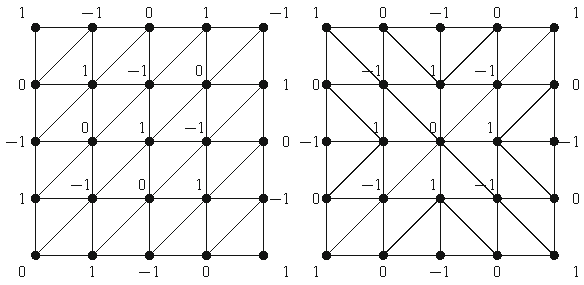
\includegraphics[width=\linewidth]{figures/Chapter_03/Fig_3_01__PDFp077__Bookp065.pdf}
  \captionof{figure}{$P_1/P_1$ 有限元的棋盘格型不稳定模态.}\label{fig:p1p1-checkerboard}
\end{elegantfigure}

\begin{example}[($P_1/P_0$ 有限元空间对)]\label{ex:p1-p0-instability}
正如\hyperref[note:infsup-not-inherited]{注记 3.52} 所指出的,压力有限元空间应当足够小,才能满足离散 inf-sup 条件.由\hyperref[ex:p1-p1-instability]{例题 3.69} 可知,$P_1/P_1$ 空间对显然不满足这一要求.乍看之下,一个直接的想法是用次数更低的多项式逼近压力,也就是用分片常数代替连续分片线性函数.$P_0$ 空间由不连续函数构成,参见\hyperref[ex:appendix-b-37]{例题 B.37}.分片常数函数很容易实现;若 $P_1/P_0$ 空间对满足离散 inf-sup 条件\cref{eq:discrete-infsup-condition},它就会是一个易于使用的选择.

对于 $P_1/P_0$ 空间对,有 $\nabla\cdot P_1\subset P_0$.根据\hyperref[note:mass-conservation-discrete-spaces]{注记 3.56},离散无散速度有限元函数还具有弱无散这一理想性质.然而,$P_1/P_0$ 空间对仍不满足离散 inf-sup 条件\cref{eq:discrete-infsup-condition}.

从\cref{fig:p1p1-checkerboard} 可见,标量值空间 $P_0$ 的维数甚至可能大于标量值空间 $P_1$ 的维数.在图示网格上,$P_1$ 有 25 个自由度(即顶点数),而 $P_0$ 有 32 个自由度(即网格单元数).相应压力有限元空间的自由度各少一个,因为离散压力还必须满足零均值条件.因此可以预期会出现伪模态;下面将详细说明.除此之外,还可能出现另一种称为锁死的现象.

先证明伪模态可能出现.为简单起见,取 $\Omega=(0,1)^2$,考虑\cref{fig:p1p1-checkerboard} 所示类型的网格,其中有 $2n^2$ 个网格单元,$n>1$.速度空间的维数是内部顶点数的两倍,而压力空间的维数等于网格单元数减去零均值约束对应的一个自由度.因此
\[
  \dim V^h-\dim Q^h
   =2(n-1)^2-(2n^2-1)=3-4n<0.
\]
于是,离散系统唯一可解的必要条件 $\dim V^h\ge\dim Q^h$ 不成立,参见\hyperref[note:finite-dimensional-saddle-point]{注记 3.7}.因此,矩阵 $B^h$ 至少有 $4n-3$ 行(等价地,$(B^h)^T$ 至少有 $4n-3$ 列)线性相关.由此可知,$Q^h$ 中存在一个维数至少为 $4n-3$ 的子空间,其中每个 $q^h$ 都满足
\[
  \begin{aligned}
    0&=\bigl\langle (B^h)^Tq^h,v^h\bigr\rangle_{(V^h)',V^h}\\
     &=b^h(v^h,q^h)=-(\nabla\cdot v^h,q^h)
       \qquad\forall v^h\in V^h.
  \end{aligned}
\]
  这正是\cref{eq:spurious-pressure-mode}.将这一例子推广到一般二维多边形区域也是可能的,见\textcite[第 189 页]{ErnGuermond2004}.

\begin{elegantfigure}[0.339\paperwidth]
  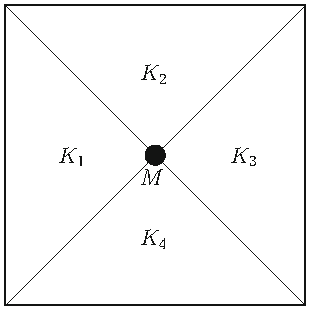
\includegraphics[width=\linewidth]{figures/Chapter_03/Fig_3_02__PDFp078__Bookp066.pdf}
  \captionof{figure}{$P_1/P_0$ 有限元的锁死网格.}\label{fig:p1p0-locking-grid}
\end{elegantfigure}

接下来说明锁死现象.仍取 $\Omega=(0,1)^2$,并用两条对角线将其剖分为四个三角形,如\cref{fig:p1p0-locking-grid} 所示.记分片常数压力检验函数 $q^h$ 在三角形 $K_i$ 上的值为 $q_i^h$,$i=1,\ldots,4$.由于四个三角形面积相等,$q^h\in L_0^2(\Omega)$ 等价于
\[
  q_1^h+q_2^h+q_3^h+q_4^h=0.
\]
因此离散压力有三个独立自由度.由离散无散空间的定义(\cref{eq:discrete-divergence-free-space}),$v^h\in V_{\mathrm{div}}^h$ 必须满足三个独立条件.然而,速度只有两个标量自由度,均位于两条对角线的交点 $M$.设 $v^h=(u^h,v^h)^T$,直接计算得到
\[
  \begin{aligned}
    \left.\nabla\cdot v^h\right|_{K_1}
     &=-\left.\nabla\cdot v^h\right|_{K_3}=\frac{u^h(M)}{2},\\
    \left.\nabla\cdot v^h\right|_{K_4}
     &=-\left.\nabla\cdot v^h\right|_{K_2}=\frac{v^h(M)}{2}.
  \end{aligned}
\]
不妨把 $q_1^h,q_2^h,q_3^h$ 作为离散压力的独立自由度,由上述零均值条件和散度公式可得
\[
\begin{aligned}
  0=(\nabla\cdot v^h,q^h)
   &=|K_1|q_1^h\left.\nabla\cdot v^h\right|_{K_1}\\
   &\quad+|K_1|q_2^h\left.\nabla\cdot v^h\right|_{K_2}\\
   &\quad+|K_1|q_3^h\left.\nabla\cdot v^h\right|_{K_3}\\
   &\quad-|K_1|(q_1^h+q_2^h+q_3^h)
         \left.\nabla\cdot v^h\right|_{K_4}\\
   &=|K_1|u^h(M)\left(\frac{q_1^h}{2}-\frac{q_3^h}{2}\right)\\
   &\qquad-|K_1|v^h(M)
         \left(\frac{q_1^h}{2}+q_2^h+\frac{q_3^h}{2}\right).
\end{aligned}
\]
此式对任意 $q_1^h,q_2^h,q_3^h$ 都成立,故 $u^h(M)=v^h(M)=0$,从而 $V_{\mathrm{div}}^h=\{0\}$.当唯一的离散无散速度是零函数时,就称发生了锁死现象.
\end{example}

\begin{elegantfigure}[0.42\paperwidth]
  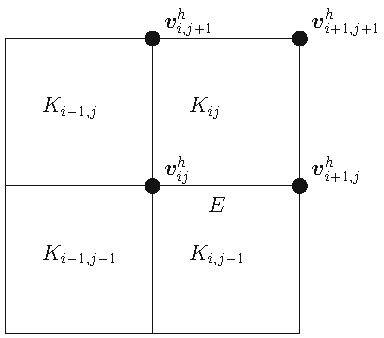
\includegraphics[width=\linewidth]{figures/Chapter_03/Fig_3_03__PDFp079__Bookp067.pdf}
  \captionof{figure}{例题 3.71 中的网格记号.}\label{fig:q1q0-nodal-indexing}
\end{elegantfigure}

\begin{example}[($Q_1/Q_0$ 有限元空间对)]\label{ex:q1-q0-instability}
令 $\Omega=(0,1)^2$,将其剖分为 $n\times n$ 个正方形,其中 $n$ 为偶数.网格单元记为 $K_{ij}$,$i,j=1,\ldots,n$,按从左至右、从下至上的字典序编号.速度有限元函数是双线性分片函数,由其在正方形顶点处的取值确定,参见\hyperref[ex:appendix-b-50]{例题 B.50}.记顶点 $(i,j)$ 处的速度值为 $v_{ij}^h=(u_{ij}^h,v_{ij}^h)^T$,见\cref{fig:q1q0-nodal-indexing}.压力由分片常数有限元函数逼近,参见\hyperref[ex:appendix-b-49]{例题 B.49};记其在 $K_{ij}$ 上的取值为 $q_{ij}^h$.

与在对应网格上将正方形沿对角线剖分所得的 $P_1/P_0$ 有限元相比,速度自由度数相同,因为两种网格的内部顶点数相同.但 $Q_0$ 压力空间的自由度数(网格单元数减一)大约只有相应 $P_0$ 空间的一半.根据\hyperref[note:infsup-not-inherited]{注记 3.52},降低 $Q^h$ 的维数或许能得到满足 inf-sup 条件的空间对.

压力有限元函数的积分均值应为零.设 $h$ 是正方形 $K_{ij}$ 的边长,则 $|K_{ij}|=h^2$,从而
\begin{equation}\label{eq:q1q0-pressure-mean}
  \sum_{i,j=1}^{n}q_{ij}^h=0.
\end{equation}

考虑单个网格单元 $K_{ij}$.分部积分可得
\[
  \int_{K_{ij}}(\nabla\cdot v^h)q_{ij}^h\,\mathrm{d}x
   =q_{ij}^h\int_{K_{ij}}\nabla\cdot v^h\,\mathrm{d}x
   =q_{ij}^h\int_{\partial K_{ij}}v^h\cdot n_{\partial K_{ij}}\,\mathrm{d}s,
\]
其中 $v^h=(u^h,v^h)^T$,$n_{\partial K_{ij}}$ 是 $\partial K_{ij}$ 上指向外侧的单位法向量.边界上的外法向量为 $\pm e_i$($i=1,2$),而 $Q_1$ 有限元函数在每条边上的限制是线性函数,所以边界积分可以用梯形公式精确计算.例如,对底边 $E$ 有
\[
  \int_E v^h\cdot n_{\partial K_{ij}}\,\mathrm{d}s
   =-\int_E v^h\cdot e_2\,\mathrm{d}s
   =-\int_E v_2^h(s)\,\mathrm{d}s
   =-\frac{h}{2}\bigl(v_{ij}^h+v_{i+1,j}^h\bigr).
\]
综合各边的贡献,得到
\[
\begin{aligned}
  \int_{K_{ij}}(\nabla\cdot v^h)q_{ij}^h\,\mathrm{d}x
   =\frac{h}{2}q_{ij}^h\bigl(&-v_{ij}^h-v_{i+1,j}^h
       +u_{i+1,j}^h+u_{i+1,j+1}^h\\
       &+v_{i+1,j+1}^h+v_{i,j+1}^h\\
       &-u_{i,j+1}^h-u_{ij}^h\bigr).
\end{aligned}
\]

接着考察与内部速度节点相关的积分贡献.边界节点不必考虑,因为速度在这些节点处为零.对于节点 $(i,j)$,$i,j=2,\ldots,n$,它是四个网格单元的顶点;这四个单元对积分的贡献分别为
\[
\begin{aligned}
  &\frac{h}{2}u_{ij}^h
     \bigl(q_{i-1,j-1}^h+q_{i-1,j}^h-q_{i,j-1}^h-q_{ij}^h\bigr),\\
  &\frac{h}{2}v_{ij}^h
     \bigl(q_{i-1,j-1}^h+q_{i,j-1}^h-q_{i-1,j}^h-q_{ij}^h\bigr).
\end{aligned}
\]
把所有单元积分相加,只是将求和重新整理为各内部节点的贡献之和.因此,条件\cref{eq:spurious-pressure-mode} 可写成
\[
\begin{aligned}
  0=(\nabla\cdot v^h,q^h)
   &=\sum_{i,j=1}^{n}(\nabla\cdot v^h,q_{ij}^h)_{K_{ij}}\\
   &=\frac{h}{2}\sum_{i,j=2}^{n}u_{ij}^h
       \bigl(q_{i-1,j-1}^h+q_{i-1,j}^h\bigr)\\
   &\quad-\frac{h}{2}\sum_{i,j=2}^{n}u_{ij}^h
       \bigl(q_{i,j-1}^h+q_{ij}^h\bigr)\\
   &\quad+\frac{h}{2}\sum_{i,j=2}^{n}v_{ij}^h
       \bigl(q_{i-1,j-1}^h+q_{i,j-1}^h\bigr)\\
   &\quad-\frac{h}{2}\sum_{i,j=2}^{n}v_{ij}^h
       \bigl(q_{i-1,j}^h+q_{ij}^h\bigr),
       \qquad\forall v^h\in V^h.
\end{aligned}
\]
特别地,令速度有限元函数只有某一个 $u_{ij}^h$ 或 $v_{ij}^h$ 非零,可知压力必须满足
\[
\begin{aligned}
  q_{i-1,j-1}^h+q_{i-1,j}^h-q_{i,j-1}^h-q_{ij}^h&=0,\\
  q_{i-1,j-1}^h+q_{i,j-1}^h-q_{i-1,j}^h-q_{ij}^h&=0,
  \qquad i,j=2,\ldots,n.
\end{aligned}
\]
将这两个条件相加、相减,得到
\begin{equation}\label{eq:q1q0-pressure-recursion}
  q_{ij}^h=q_{i-1,j-1}^h,
  \qquad q_{i,j-1}^h=q_{i-1,j}^h,
  \qquad i,j=2,\ldots,n.
\end{equation}

乍看之下,依据\cref{eq:q1q0-pressure-recursion} 可以自由选取两个压力值:例如令 $K_{11}$ 上的压力为 $\alpha\in\mathbb{R}$,则所有指标和为偶数的网格单元都取同一值;再令另一个网格单元(其指标和为奇数)上的压力为 $\beta$,则另一半网格单元都取此值.假定 $n$ 为偶数,才能使两组网格单元的数量相同.由零均值条件\cref{eq:q1q0-pressure-mean} 可得 $0=\frac{n^2}{2}(\alpha+\beta)$,故 $\beta=-\alpha$.因此,任取 $\alpha\ne0$,便得到满足\cref{eq:spurious-pressure-mode} 的非零压力有限元函数;一个例子见\cref{fig:q1q0-checkerboard}.这种不稳定性也称为棋盘格不稳定.
\end{example}

\begin{elegantfigure}[0.338\paperwidth]
  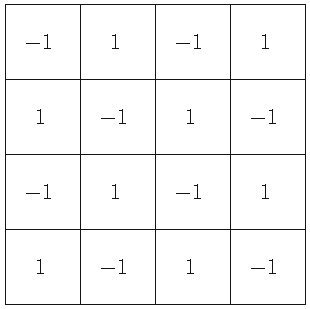
\includegraphics[width=\linewidth]{figures/Chapter_03/Fig_3_04__PDFp081__Bookp069.pdf}
  \captionof{figure}{$Q_1/Q_0$ 有限元的棋盘格型不稳定模态.}\label{fig:q1q0-checkerboard}
\end{elegantfigure}

\begin{note}[改善 $Q_1/Q_0$ 有限元稳定性的改造]\label{note:q1q0-stabilization}
\begin{itemize}
  \item 既然伪模态可以明确刻画,一种做法是缩小压力有限元空间,只保留 $L^2(\Omega)$ 正交于该模态的函数.已有结果表明,这样可以得到满足 inf-sup 条件的有限元空间对.不过,inf-sup 参数依赖于网格宽度,满足 $\beta_{\mathrm{is}}^h=Ch$,其中 $C$ 与 $h$ 无关,参见\textcite[第 II 章第 3 节]{GiraultRaviart1986}.有限元误差估计中会出现 $\beta_{\mathrm{is}}^h$ 的倒数,因此这种方法可能不收敛.
  \item \textcite{BolandNicolaides1985} 提出了对压力有限元空间的进一步改造,使空间对关于 $h$ 一致稳定;细节也可见\textcite[第 167 页]{GiraultRaviart1986}.但据我们所知,Boland 和 Nicolaides 的方法在实践中并未得到应用.
  \item 在非常特殊的网格上,可以证明 $Q_1/Q_0$ 空间对满足离散 inf-sup 条件,见\textcite{Stenberg1984}.
\end{itemize}
\end{note}

\begin{example}[($P_k/P_{k-1}^{\mathrm{disc}}$,$k\ge2$,特殊宏单元)]\label{ex:scott-vogelius-macroelement}
考虑\cref{fig:scott-vogelius-macroelement} 所示网格上的空间对 $P_k/P_{k-1}^{\mathrm{disc}}$,$k\ge2$,特别是粗线框圈出的宏单元.宏单元两条对角线应分别平行于坐标轴.这个空间对称为 Scott--Vogelius 有限元,见\textcite{ScottVogelius1985}.

\begin{elegantfigure}[0.64\paperwidth]
  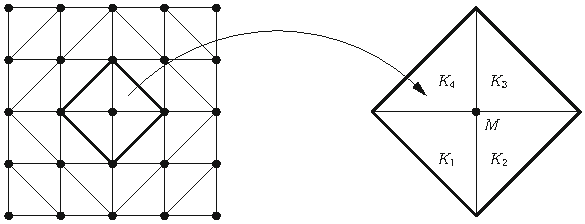
\includegraphics[width=\linewidth]{figures/Chapter_03/Fig_3_05__PDFp082__Bookp070.pdf}
  \captionof{figure}{$P_k/P_{k-1}^{\mathrm{disc}}$ 有限元的网格;粗线框标出宏单元.}\label{fig:scott-vogelius-macroelement}
\end{elegantfigure}

若 $v^h\in P_k$,则 $\nabla\cdot v^h\in P_{k-1}^{\mathrm{disc}}=Q^h$.因此,由\hyperref[note:mass-conservation-discrete-spaces]{注记 3.56} 可知,$P_k/P_{k-1}^{\mathrm{disc}}$ 空间对中的离散无散速度有限元函数也是弱无散的,这是一个理想性质.不过,在图示网格上,$P_k/P_{k-1}^{\mathrm{disc}}$ 并不满足离散 inf-sup 条件.

取 $v^h=(v_1^h,v_2^h)^T\in V_{\mathrm{div}}^h$.由于 $v^h$ 连续,其沿网格边切向的导数 $\nabla v^h\cdot t$ 也连续.利用切向量是笛卡尔坐标单位向量,可得
\[
\begin{aligned}
  \left.\frac{\partial v_2^h}{\partial y}\right|_{K_1}
   &=\left.\frac{\partial v_2^h}{\partial y}\right|_{K_2},
  &\left.\frac{\partial v_1^h}{\partial x}\right|_{K_2}
   &=\left.\frac{\partial v_1^h}{\partial x}\right|_{K_3},\\
  \left.\frac{\partial v_2^h}{\partial y}\right|_{K_3}
   &=\left.\frac{\partial v_2^h}{\partial y}\right|_{K_4},
  &\left.\frac{\partial v_1^h}{\partial x}\right|_{K_4}
   &=\left.\frac{\partial v_1^h}{\partial x}\right|_{K_1}.
\end{aligned}
\]
这些等式在顶点 $M$ 处仍成立.再利用 $K_2,K_3,K_4$ 上逐点散度为零的约束,可得
\[
\begin{aligned}
  \left.\nabla\cdot v^h\right|_{K_1}(M)
   &=\left.\frac{\partial v_1^h}{\partial x}\right|_{K_1}(M)
     +\left.\frac{\partial v_2^h}{\partial y}\right|_{K_1}(M)\\
   &=\left.\frac{\partial v_1^h}{\partial x}\right|_{K_1}(M)
     +\left.\frac{\partial v_2^h}{\partial y}\right|_{K_2}(M)\\
   &=\left.\frac{\partial v_1^h}{\partial x}\right|_{K_1}(M)
     -\left.\frac{\partial v_1^h}{\partial x}\right|_{K_2}(M)\\
   &=\left.\frac{\partial v_1^h}{\partial x}\right|_{K_1}(M)
     -\left.\frac{\partial v_1^h}{\partial x}\right|_{K_3}(M)\\
   &=\left.\frac{\partial v_1^h}{\partial x}\right|_{K_1}(M)
     +\left.\frac{\partial v_2^h}{\partial y}\right|_{K_3}(M)\\
   &=\left.\frac{\partial v_1^h}{\partial x}\right|_{K_1}(M)
     +\left.\frac{\partial v_2^h}{\partial y}\right|_{K_4}(M)\\
   &=\left.\frac{\partial v_1^h}{\partial x}\right|_{K_1}(M)
     -\left.\frac{\partial v_1^h}{\partial x}\right|_{K_4}(M)=0.
\end{aligned}
\]
这说明,$v^h$ 在宏单元 $K_1$ 上的散度为零这一条件,可由边上的切向导数连续性以及 $K_2,K_3,K_4$ 上散度为零推出.由于 $v^h$ 弱无散,故
\begin{equation}\label{eq:scott-vogelius-local-weak-divergence}
  (\nabla\cdot v^h,q^h)_{K_1}=0
  \qquad\forall q^h\in Q^h(K_1).
\end{equation}
由\cref{eq:scott-vogelius-local-weak-divergence} 可知,为确定 $\nabla\cdot v^h|_{K_1}\in P_{k-1}(K_1)$,需要 $\dim P_{k-1}(K_1)=\dim Q^h(K_1)=k(k+1)/2$ 个条件;此外还独立得到 $\nabla\cdot v^h|_{K_1}(M)=0$.因此,\cref{eq:scott-vogelius-local-weak-divergence} 中有一个条件多余.舍去其中一个条件后,$K_1$ 上的一个压力自由度便无法由\cref{eq:scott-vogelius-local-weak-divergence} 确定,成为伪自由度.
\end{example}

\begin{note}[其他网格上的 Scott--Vogelius 有限元]\label{note:scott-vogelius-other-meshes}
例题\hyperref[ex:scott-vogelius-macroelement]{3.73} 中的特殊网格对于证明 Scott--Vogelius 有限元不满足离散 inf-sup 条件至关重要.可以证明,在某种意义下结构性较弱的网格上,次数充分高的 Scott--Vogelius 有限元空间对满足离散 inf-sup 条件,见\hyperref[sec:scott-vogelius]{第 3.6.3 节}.
\end{note}

\begin{note}[绕开离散 inf-sup 条件]\label{note:circumvent-discrete-infsup}
如\hyperref[note:low-order-finite-element-pairs]{注记 3.67} 所述,低阶有限元空间很受欢迎.为将它们用于不可压缩流模拟,人们提出了多种不必满足离散 inf-sup 条件\cref{eq:discrete-infsup-condition} 的方法.其基本思想是在连续性方程中加入双线性型,使压力之间产生耦合,从而消除问题的鞍点结构.第 5.3 节讨论的 PSPG 方法就是一例.当然,在连续性方程中加入额外项会导致(离散)质量守恒遭到破坏.
\end{note}

\section{检验离散 inf-sup 条件的技巧}\label{sec:checking-discrete-infsup}

\begin{note}[内容]\label{note:fortin-section-contents}
本节介绍若干检验离散 inf-sup 条件\cref{eq:discrete-infsup-condition}(或等价的\cref{eq:discrete-infsup-condition-equivalent})的方法,并在第 3.6 节将其中一些方法用于具体的有限元空间对.关于证明离散 inf-sup 条件的技巧及相应结果,较全面的综述可见\textcite{Boffi2008},以及\textcite[第 8.4、8.5 节]{Boffi2013}.
\end{note}

\subsection{Fortin 算子}\label{subsec:fortin-operator}

\begin{note}[连续与离散 inf-sup 条件之间的联系]\label{note:continuous-discrete-infsup-connection}
对于协调有限元空间,可以借助连续 inf-sup 条件\cref{eq:infsup-v-q} 检验离散 inf-sup 条件\cref{eq:discrete-infsup-condition}.下面的引理说明了这两个条件之间的联系.该结果源于\textcite{Fortin1977};它还可推广到 Banach 空间,见\textcite[引理 4.19]{ErnGuermond2004}.某些非协调情形也有相应推广,见第\hyperref[sec:lowest-order-nonconforming]{3.6.5 节}.对于协调有限元空间,$b^h(\cdot,\cdot)=b(\cdot,\cdot)$.
\index{Fortin 算子}
\end{note}

\begin{lemma}[检验离散 inf-sup 条件的 Fortin 判据]\label{lem:fortin-criterion}
设 $V$、$Q$ 和双线性型 $b(\cdot,\cdot)$ 满足注记\hyperref[note:abstract-saddle-point-problem]{3.3} 中的假设,且 inf-sup 条件\cref{eq:infsup-v-q} 成立.考虑协调空间 $V^h\subset V$ 和 $Q^h\subset Q$.则 $V^h$ 与 $Q^h$ 满足离散 inf-sup 条件\cref{eq:discrete-infsup-condition},当且仅当存在一个与 $h$ 无关的常数 $\gamma^h>0$,使得对每个 $v\in V$,都存在 $P_{\mathrm{For}}^h v\in V^h$ 满足
\begin{equation}\label{eq:fortin-property}
  b(v,q^h)=b(P_{\mathrm{For}}^h v,q^h)
  \quad\forall q^h\in Q^h,
  \qquad
  \|P_{\mathrm{For}}^h v\|_V\le \gamma^h\|v\|_V.
\end{equation}
\end{lemma}

\begin{proof}
先假设\cref{eq:fortin-property} 成立.任取 $q^h\in Q^h$.由于 $P_{\mathrm{For}}^h v\in V^h$,利用\cref{eq:fortin-property} 及连续 inf-sup 条件\cref{eq:infsup-v-q},有
\[
\begin{aligned}
  \sup_{v^h\in V^h\setminus\{0\}}
    \frac{b(v^h,q^h)}{\|v^h\|_V}
  &\ge
  \sup_{v\in V\setminus\{0\}}
    \frac{b(P_{\mathrm{For}}^h v,q^h)}
         {\|P_{\mathrm{For}}^h v\|_V}\\
  &=\sup_{v\in V\setminus\{0\}}
    \frac{b(v,q^h)}{\|P_{\mathrm{For}}^h v\|_V}
  \ge \frac{\beta_{\mathrm{is}}}{\gamma^h}
       \|q^h\|_Q .
\end{aligned}
\]
这正是离散 inf-sup 条件\cref{eq:discrete-infsup-condition},且其参数满足 $\beta_{\mathrm{is}}^h\ge \beta_{\mathrm{is}}/\gamma^h$.

反过来,假设离散 inf-sup 条件\cref{eq:discrete-infsup-condition} 成立.将 $b(\cdot,\cdot)$ 从 $V\times Q$ 限制到 $V\times Q^h$,便得到连续线性算子
\[
  \widetilde B\in\mathcal{L}\bigl(V,(Q^h)'\bigr),
  \qquad
  \langle\widetilde Bv,q^h\rangle_{(Q^h)',Q^h}
  :=b(v,q^h).
\]
根据定义,对所有 $v\in V$ 都有 $\widetilde Bv\in(Q^h)'$.由于离散 inf-sup 条件成立,由引理\ref{lem:inf-sup-condition}(iii)可知,\cref{eq:discrete-divergence-operator} 中定义的离散散度算子 $B^h$ 是从 $(V_{\mathrm{div}}^h)^\perp$ 到 $(Q^h)'$ 的同构;特别地,它是满射.于是,对给定的 $v\in V$,存在 $\widetilde v^h\in(V_{\mathrm{div}}^h)^\perp$,使得
\[
  \langle B^h\widetilde v^h,q^h\rangle_{(Q^h)',Q^h}
  =\langle\widetilde Bv,q^h\rangle_{(Q^h)',Q^h}
  \quad\forall q^h\in Q^h.
\]
因此,对所有在 $(V_{\mathrm{div}}^h)^\perp$ 上的正交投影等于 $\widetilde v^h$ 的 $v^h\in V^h$,均有
\begin{equation}\label{eq:fortin-projection-pairing}
  \langle B^h v^h,q^h\rangle_{(Q^h)',Q^h}
  =\langle\widetilde Bv,q^h\rangle_{(Q^h)',Q^h}
  \quad\forall q^h\in Q^h.
\end{equation}
取其中一个这样的函数作为 $P_{\mathrm{For}}^h v$,则\cref{eq:fortin-projection-pairing} 等价于
\[
  b(P_{\mathrm{For}}^h v,q^h)=b(v,q^h)
  \quad\forall q^h\in Q^h.
\]

由引理\ref{lem:inf-sup-condition}(iii)、$Q^h$ 上范数的定义、双线性型 $b(\cdot,\cdot)$ 的范数\cref{eq:bilinear-form-norms},以及其有界性估计(引理\ref{lem:bounded-bilinear-form-b}),可得
\[
\begin{aligned}
  \|P_{\mathrm{For}}^h v\|_V
  &\le \frac{1}{\beta_{\mathrm{is}}^h}
       \|B^hP_{\mathrm{For}}^h v\|_{(Q^h)'}\\
  &=\frac{1}{\beta_{\mathrm{is}}^h}
    \sup_{q^h\in Q^h\setminus\{0\}}
      \frac{\langle B^hP_{\mathrm{For}}^h v,q^h\rangle}
           {\|q^h\|_Q}\\
  &=\frac{1}{\beta_{\mathrm{is}}^h}
    \sup_{q^h\in Q^h\setminus\{0\}}
      \frac{b(v,q^h)}{\|q^h\|_Q}\\
  &\le \frac{\|b\|}{\beta_{\mathrm{is}}^h}\|v\|_V
   =\gamma^h\|v\|_V,
\end{aligned}
\]
从而得到\cref{eq:fortin-property}.证毕.
\end{proof}

\begin{note}[关于条件(3.76)]\label{note:fortin-excludes-spurious-pressure}
条件\cref{eq:spurious-pressure-mode} 一旦成立,就意味着离散 inf-sup 条件被破坏;若\cref{eq:fortin-property} 成立,则不可能满足\cref{eq:spurious-pressure-mode}.事实上,假设存在 $q^h\in Q^h$,使得对所有 $v^h\in V^h$ 都有 $b(v^h,q^h)=0$.由\cref{eq:fortin-property} 可知,对所有 $v\in V$ 都有 $b(v,q^h)=0$,因为 $P_{\mathrm{For}}^h v\in V^h$.又因 $q^h\in Q$,且 $V$ 与 $Q$ 满足 inf-sup 条件\cref{eq:infsup-v-q},故 $q^h=0$.因此,不存在非零的 $q^h\in Q^h$ 满足\cref{eq:spurious-pressure-mode}.
\end{note}

\begin{note}[梯度算子的核]\label{note:fortin-gradient-kernels}
由\cref{eq:fortin-property} 的第一部分可得
\[
  \ker(\operatorname{grad}^h)\subseteq\ker(\operatorname{grad}).
\]
为证此包含关系,取 $q^h\in\ker(\operatorname{grad}^h)$,于是对所有 $v^h\in V^h$,有 $b(v^h,q^h)=0$.由于对每个 $v\in V$ 都有 $P_{\mathrm{For}}^h v\in V^h$,故对所有 $v\in V$ 均有 $b(v,q^h)=0$.因此 $q^h\in\ker(\operatorname{grad})$.
\end{note}

\begin{note}[构造 Fortin 算子的一种方法]\label{note:fortin-construction}
有时可以借助两个线性算子 $P_1^h,P_2^h\in\mathcal{L}(V,V^h)$ 构造线性 Fortin 算子 $P_{\mathrm{For}}^h$.假设
\begin{align}
  \|P_1^h v\|_V&\le C_1\|v\|_V
      &&\forall v\in V,\label{eq:fortin-p1-bound}\\
  \|P_2^h(I-P_1^h)v\|_V&\le C_2\|v\|_V
      &&\forall v\in V,\label{eq:fortin-p2-bound}\\
  b(v-P_2^h v,q^h)&=0
      &&\forall v\in V,\ \forall q^h\in Q^h,\label{eq:fortin-p2-moment}
\end{align}
其中 $C_1,C_2$ 均与 $h$ 无关.定义
\begin{equation}\label{eq:fortin-operator-construction}
  P_{\mathrm{For}}^h\in\mathcal{L}(V,V^h),
  \qquad
  v\longmapsto P_1^h v+P_2^h(v-P_1^h v).
\end{equation}
则 $P_{\mathrm{For}}^h$ 是 Fortin 算子.
\end{note}

\begin{lemma}[算子(3.87)的性质]\label{lem:fortin-operator-construction}
由\cref{eq:fortin-operator-construction} 定义的算子满足\cref{eq:fortin-property}.
\end{lemma}

\begin{proof}
由\cref{eq:fortin-operator-construction},先对 $P_1^h v$ 使用\cref{eq:fortin-p2-moment},再对 $v$ 使用一次\cref{eq:fortin-p2-moment},可得对所有 $q^h\in Q^h$,
\[
\begin{aligned}
  b(P_{\mathrm{For}}^h v,q^h)
  &=b\bigl(P_1^h v+P_2^h(v-P_1^h v),q^h\bigr)\\
  &=b\bigl(P_1^h v-P_2^hP_1^h v,q^h\bigr)
    +b(P_2^h v,q^h)\\
  &=b(P_2^h v,q^h)=b(v,q^h).
\end{aligned}
\]
再由三角不等式以及\cref{eq:fortin-p1-bound,eq:fortin-p2-bound},得到
\[
\begin{aligned}
  \|P_{\mathrm{For}}^h v\|_V
  &\le \|P_1^h v\|_V+
        \|P_2^h(v-P_1^h v)\|_V\\
  &\le C_1\|v\|_V+C_2\|v\|_V
   =\gamma^h\|v\|_V,
\end{aligned}
\qquad\gamma^h:=C_1+C_2.
\]
故\cref{eq:fortin-property} 成立.证毕.
\end{proof}

\begin{note}[Fortin 算子的较精细构造]\label{note:fortin-detailed-construction}
通常可令 $P_1^h$ 取 Clément 插值算子 $P_{\mathrm{Cle}}^h$(\hyperref[eq:appendix-c-17]{式(C.17)}),并作适当修改以保持齐次 Dirichlet 边界条件,见注记\hyperref[note:appendix-c-22]{C.22}.此时,对 $P_2^h$ 的条件\cref{eq:fortin-p2-bound} 可由下列局部估计替代:
\begin{equation}\label{eq:fortin-local-p2-bound}
  \|P_2^h v\|_{H^1(K)}
  \le C\left(h_K^{-1}\|v\|_{L^2(K)}
              +|v|_{H^1(K)}\right),
  \quad\forall K\in\mathcal{T}^h,\ \forall v\in V,
\end{equation}
其中常数 $C$ 与 $h_K$ 无关.
\end{note}

\begin{lemma}[由(C.17)、(3.86)和(3.88)构造的 Fortin 算子的性质]\label{lem:clement-fortin-property}
设 $\{\mathcal{T}^h\}$ 是一族准一致三角剖分(quasi-uniform triangulations).令 $P_1^h=P_{\mathrm{Cle}}^h$ 为经修改、可保持齐次 Dirichlet 边界条件的 Clément 插值算子(\hyperref[eq:appendix-c-17]{C.17}),并设 $P_2^h$ 满足\cref{eq:fortin-p2-moment,eq:fortin-local-p2-bound}.则由\cref{eq:fortin-operator-construction} 定义的 $P_{\mathrm{For}}^h$ 是一个 Fortin 算子.
\end{lemma}

\begin{proof}
\cref{eq:fortin-property} 的第一项性质可按引理\ref{lem:fortin-operator-construction} 的证明得到,因为该证明只用到了\cref{eq:fortin-p2-moment,eq:fortin-operator-construction}.下面证明其中的第二项性质,且所得常数 $\gamma^h$ 与 $h$ 无关.

由剖分族的准一致性可知,对每个 $K$,邻域 $\Omega_K$ 中的网格单元数有一个与剖分无关的上界;此外,$\Omega_K$ 的直径可由 $Ch_K$ 控制,其中常数 $C$ 与 $\mathcal{T}^h$ 无关,见图\hyperref[fig:appendix-c-1]{C.1}.利用\cref{eq:fortin-operator-construction}、三角不等式、\cref{eq:fortin-local-p2-bound},以及在 $k=0,l=1$ 和 $k=l=1$ 时的估计(\hyperref[eq:appendix-c-18]{C.18}),可得
\[
\begin{aligned}
  \|P_{\mathrm{For}}^h v\|_V^2
  &=|P_{\mathrm{For}}^h v|_{H^1(\Omega)}^2\\
  &\le 2|P_{\mathrm{Cle}}^h v|_{H^1(\Omega)}^2
       +2|P_2^h(v-P_{\mathrm{Cle}}^h v)|_{H^1(\Omega)}^2\\
  &\le C\left(|P_{\mathrm{Cle}}^h v-v|_{H^1(\Omega)}^2
                 +|v|_{H^1(\Omega)}^2\right)\\
  &\qquad+2\sum_{K\in\mathcal{T}^h}
        |P_2^h(v-P_{\mathrm{Cle}}^h v)|_{H^1(K)}^2\\
  &\le C\left(\sum_{K\in\mathcal{T}^h}
          |P_{\mathrm{Cle}}^h v-v|_{H^1(K)}^2
          +|v|_{H^1(\Omega)}^2\right)\\
  &\qquad+C\sum_{K\in\mathcal{T}^h}
       \left(h_K^{-2}\|v-P_{\mathrm{Cle}}^h v\|_{L^2(K)}^2
       +|v-P_{\mathrm{Cle}}^h v|_{H^1(K)}^2\right)\\
  &\le C\left(|v|_{H^1(\Omega)}^2
       +3\sum_{K\in\mathcal{T}^h}|v|_{H^1(\Omega_K)}^2\right)\\
  &\le C\|\nabla v\|_{L^2(\Omega)}^2\\
  &=C\|v\|_V^2.
\end{aligned}
\]
证毕.
\end{proof}

\begin{note}[非协调离散]\label{note:fortin-nonconforming}
Fortin 算子的思想也用于非协调方法中证明离散 inf-sup 条件.例如,证明 Crouzeix--Raviart 有限元空间对(见定理\hyperref[thm:crouzeix-raviart-infsup]{3.151})时,就用到了这一思想,相关关系见\hyperref[eq:crouzeix-raviart-fortin-identity]{式(3.144)}和\hyperref[eq:crouzeix-raviart-fortin-bound]{式(3.145)}.
\end{note}

\subsection{将离散压力分解为分片常数部分与余项}\label{subsec:pressure-splitting}

\begin{note}[基本思路]\label{note:pressure-splitting-approach}
注记\hyperref[note:infsup-not-inherited]{3.52} 已指出,较小的压力有限元空间有利于满足离散 inf-sup 条件\cref{eq:discrete-infsup-condition},或等价的\cref{eq:discrete-infsup-condition-equivalent}.给定一个三角剖分,较小的有限元空间是分片常数空间与 $L_0^2(\Omega)$ 的交.这里假设速度空间与分片常数压力空间组成的空间对 $V^h/P_0$ 或 $V^h/Q_0$ 满足离散 inf-sup 条件.然后,将离散 inf-sup 条件\cref{eq:discrete-infsup-condition-equivalent} 右侧的压力有限元函数分解为分片常数部分 $\bar q^h$ 与余项:
\index{分片常数压力空间}
\[
  q^h=\bar q^h+(q^h-\bar q^h).
\]
对于这个余项,也假设有一个 inf-sup 条件,最终由此推出所需的离散 inf-sup 条件.其思路是,分别为分片常数部分和余项证明 inf-sup 条件都相对容易.该方法由\textcite{BrezziBathe1990} 提出.
\end{note}

\begin{lemma}[$L^2(\Omega)$ 投影到分片常数有限元空间的性质]\label{lem:piecewise-constant-projection}
\index{$L^2$ 投影!分片常数空间}
设 $q^h\in Q^h$,并以 $\bar q^h$ 表示它在 $L^2(\Omega)$ 中到 $P_0$ 或 $Q_0$ 的投影,即
\begin{equation}\label{eq:piecewise-constant-projection-orthogonality}
  (q^h-\bar q^h,r^h)=0
  \qquad\forall r^h\in P_0\ (\text{或 }Q_0).
\end{equation}
则
\[
  \left.\bar q^h\right|_K
  =\frac{1}{|K|}\int_K q^h(x)\,\mathrm{d}x
  \qquad\forall K\in\mathcal{T}^h,
\]
其中 $|K|$ 表示 $K$ 的测度,并且 $\bar q^h\in L_0^2(\Omega)$.
\end{lemma}

\begin{proof}
利用 $\bar q^h$ 和 $r^h$ 都是分片常数,有
\[
\begin{aligned}
  (q^h,r^h)
  &=\sum_{K\in\mathcal{T}^h}(q^h,r^h)_K\\
  &=\sum_{K\in\mathcal{T}^h}
      \left.r^h\right|_K\int_K q^h(x)\,\mathrm{d}x,
\end{aligned}
\]
另一方面,
\[
\begin{aligned}
  (\bar q^h,r^h)
  &=\sum_{K\in\mathcal{T}^h}(\bar q^h,r^h)_K\\
  &=\sum_{K\in\mathcal{T}^h}
      \left.r^h\right|_K\left.\bar q^h\right|_K|K|.
\end{aligned}
\]
将这两个表达式代入\cref{eq:piecewise-constant-projection-orthogonality},即得 $\bar q^h|_K$ 的公式.再利用该公式以及 $q^h\in L_0^2(\Omega)$,可知 $\bar q^h$ 的均值为零:
\[
\begin{aligned}
  \int_\Omega\bar q^h(x)\,\mathrm{d}x
  &=\sum_{K\in\mathcal{T}^h}\int_K\bar q^h(x)\,\mathrm{d}x\\
  &=\sum_{K\in\mathcal{T}^h}
      \left.\bar q^h\right|_K\int_K\mathrm{d}x\\
  &=\sum_{K\in\mathcal{T}^h}
      \frac{1}{|K|}\int_Kq^h(x)\,\mathrm{d}x\int_K\mathrm{d}x\\
  &=\int_\Omega q^h(x)\,\mathrm{d}x=0.
\end{aligned}
\]
证毕.
\end{proof}

\begin{note}[一种改进的 inf-sup 条件]\label{note:modified-infsup-condition}
\index{改进的 inf-sup 条件}
这种方法的核心是如下形式的 inf-sup 条件:
\begin{equation}\label{eq:modified-infsup-condition}
  \sup_{v^h\in V^h\setminus\{0\}}
    \frac{b^h(v^h,q^h)}{\|v^h\|_{V^h}}
  \ge\beta_1\|q^h-\bar q^h\|_Q
  \qquad\forall q^h\in Q^h,
\end{equation}
其中 $\beta_1>0$ 与网格宽度无关.由引理\ref{lem:piecewise-constant-projection} 可知,$q^h-\bar q^h\in L_0^2(\Omega)$.首先,由这一表述可见,若能找到满足\cref{eq:spurious-pressure-mode} 的 $q^h\in Q^h$,则\cref{eq:modified-infsup-condition} 不可能成立:此时左端为零,而在本节假设分片常数压力空间对稳定的前提下,右端不为零.因此,\cref{eq:modified-infsup-condition} 可排除足以说明 $V^h/Q^h$ 不满足离散 inf-sup 条件的情形.另一方面,\cref{eq:modified-infsup-condition} 弱于离散 inf-sup 条件.为简单起见,考虑准一致网格.由 $L^2(\Omega)$ 投影的性质(\hyperref[eq:appendix-c-28]{C.28})和逆不等式(\hyperref[eq:appendix-c-35]{C.35}),有
\[
\begin{aligned}
  \|q^h-\bar q^h\|_Q
  &=\left(\sum_{K\in\mathcal{T}^h}
        \|q^h-\bar q^h\|_{L^2(K)}^2\right)^{1/2}\\
  &\le C\left(\sum_{K\in\mathcal{T}^h}
        h_K^2\|\nabla q^h\|_{L^2(K)}^2\right)^{1/2}\\
  &\le C\left(\sum_{K\in\mathcal{T}^h}
        \|q^h\|_{L^2(K)}^2\right)^{1/2}
   =C\|q^h\|_Q.
\end{aligned}
\]
因此,若\cref{eq:discrete-infsup-condition}(或等价的\cref{eq:discrete-infsup-condition-equivalent})成立,则\cref{eq:modified-infsup-condition} 也成立.
\end{note}

\begin{theorem}[基于分片常数压力 inf-sup 条件的离散 inf-sup 条件充分条件]\label{thm:pressure-splitting-infsup}
假设速度空间与分片常数压力空间 $V^h/P_0$ 或 $V^h/Q_0$ 满足离散 inf-sup 条件
\begin{equation}\label{eq:piecewise-constant-infsup}
  \sup_{v^h\in V^h\setminus\{0\}}
    \frac{b^h(v^h,q^h)}{\|v^h\|_{V^h}}
  \ge\beta_0\|q^h\|_Q
  \qquad\forall q^h\in P_0\ (\text{或 }Q_0),
\end{equation}
其中 $\beta_0>0$ 与 $h$ 无关.此外,假设\cref{eq:modified-infsup-condition} 成立,且 $\beta_1$ 与 $h$ 无关.则离散 inf-sup 条件\cref{eq:discrete-infsup-condition} 或\cref{eq:discrete-infsup-condition-equivalent} 成立,并且其参数满足
\[
  \beta_{\mathrm{is}}^h
  =\frac{\beta_0\beta_1}{\widetilde C+\beta_0+\beta_1}>0,
\]
其中协调速度空间对应 $\widetilde C=1$,非协调速度空间对应 $\widetilde C=\sqrt{d}$.
\end{theorem}

\begin{proof}
由于和的上确界不大于各项上确界之和,有
\[
  \sup A=\sup\bigl((A+B)-B\bigr)
  \le \sup(A+B)+\sup B,
\]
从而
\begin{equation}\label{eq:sup-sum-lower-bound}
  \sup(A+B)\ge\sup A-\sup B.
\end{equation}
任取 $q^h\in Q^h$.将压力分解为 $\bar q^h+(q^h-\bar q^h)$,并应用\cref{eq:sup-sum-lower-bound,eq:piecewise-constant-infsup} 以及协调速度空间情形的估计(3.41)或非协调速度空间情形的估计(3.40),得到
\begin{equation}\label{eq:pressure-splitting-infsup-first-estimate}
\begin{aligned}
  \sup_{v^h\in V^h\setminus\{0\}}
    \frac{b^h(v^h,q^h)}{\|v^h\|_{V^h}}
  &\ge
    \sup_{v^h\in V^h\setminus\{0\}}
      \frac{b^h(v^h,\bar q^h)}{\|v^h\|_{V^h}}\\
  &\qquad-
    \sup_{v^h\in V^h\setminus\{0\}}
      \frac{b^h(v^h,q^h-\bar q^h)}{\|v^h\|_{V^h}}\\
  &\ge \beta_0\|\bar q^h\|_Q\\
  &\qquad-
    \sup_{v^h\in V^h\setminus\{0\}}
        \frac{\|\nabla\cdot v^h\|_{L^2(\Omega)}
              \|q^h-\bar q^h\|_Q}{\|v^h\|_{V^h}}\\
  &\ge \beta_0\|\bar q^h\|_Q
      -\widetilde C\|q^h-\bar q^h\|_Q.
\end{aligned}
\end{equation}
对于非协调速度有限元空间,第二行中的 $\|\nabla\cdot v^h\|_{L^2(\Omega)}$ 应改为各网格单元上的相应范数平方和,并在每个单元上应用估计(3.40).

现在结合\cref{eq:modified-infsup-condition,eq:pressure-splitting-infsup-first-estimate},可得
\[
\begin{aligned}
  \sup_{v^h\in V^h\setminus\{0\}}
    \frac{b^h(v^h,q^h)}{\|v^h\|_{V^h}}
  &\ge \beta_1\|q^h-\bar q^h\|_Q\\
  &\ge \beta_1\left(
      \frac{\beta_0}{\widetilde C}\|\bar q^h\|_Q
      -\frac{1}{\widetilde C}
       \sup_{v^h\in V^h\setminus\{0\}}
        \frac{b^h(v^h,q^h)}{\|v^h\|_{V^h}}
       \right).
\end{aligned}
\]
移项后得到
\begin{equation}\label{eq:pressure-splitting-mean-infsup}
  \sup_{v^h\in V^h\setminus\{0\}}
    \frac{b^h(v^h,q^h)}{\|v^h\|_{V^h}}
  \ge
  \frac{\beta_0\beta_1}{\widetilde C+\beta_1}
       \|\bar q^h\|_Q.
\end{equation}

再在\cref{eq:modified-infsup-condition} 中使用三角不等式,并代入\cref{eq:pressure-splitting-mean-infsup},可得
\[
\begin{aligned}
  \sup_{v^h\in V^h\setminus\{0\}}
    \frac{b^h(v^h,q^h)}{\|v^h\|_{V^h}}
  &\ge \beta_1\|q^h\|_Q-\beta_1\|\bar q^h\|_Q\\
  &\ge \beta_1\|q^h\|_Q
   -\frac{\widetilde C+\beta_1}{\beta_0}
      \sup_{v^h\in V^h\setminus\{0\}}
        \frac{b^h(v^h,q^h)}{\|v^h\|_{V^h}}.
\end{aligned}
\]
将最后一项移至左侧,并注意 $q^h$ 任意,便得到定理陈述中的离散 inf-sup 条件及其参数 $\beta_{\mathrm{is}}^h$.证毕.
\end{proof}

\begin{note}[关于条件(3.90)]\label{note:modified-infsup-condition-comments}
\index{拼块检验}
\begin{itemize}
  \item \textcite{BrezziBathe1990} 提出了一种所谓的拼块检验,用于检验条件\cref{eq:modified-infsup-condition}.
\item \textcite{BrezziBathe1990} 还给出了另一种情形,在该情形下条件\cref{eq:modified-infsup-condition} 可推出离散 inf-sup 条件,见定理\hyperref[thm:brezzi-bathe-continuous-pressure]{3.96}.
\end{itemize}
\end{note}

\subsection{协调速度空间与连续压力空间的方法}\label{subsec:conforming-velocity-continuous-pressure}

\begin{note}[内容]\label{note:continuous-pressure-criteria}
\index{连续压力空间}
本节介绍两种判据,用于在压力空间由连续有限元函数(continuous finite element functions)组成时检验离散 inf-sup 条件\cref{eq:discrete-infsup-condition} 或\cref{eq:discrete-infsup-condition-equivalent}.第一种判据由 Verfürth(1984)证明,第二种由 Brezzi 和 Bathe(1990)证明;可以看出,这两种判据在一定程度上等价.

\index{分部积分}
\index{压力跳跃}
本节为推导离散 inf-sup 条件,需要对连续函数 $v$ 与离散压力 $q^h$ 所构成的项 $b^h(v,q^h)$ 作分部积分(integration by parts).一般而言,这会产生网格单元各个面的离散压力跳跃项(jumps of the discrete pressure);压力空间的光滑性假设 $Q^h\subset H^1(\Omega)$ 保证这些跳跃项为零.

以下假设 $V^h\subset V$,因此 $b^h(\cdot,\cdot)=b(\cdot,\cdot)$ 且 $\|\cdot\|_{V^h}=\|\cdot\|_V$.
\end{note}

\begin{lemma}[上确界的下界]\label{lem:continuous-pressure-supremum-lower-bound}
设 $\{\mathcal{T}^h\}$ 是准一致三角剖分族,且 $V^h\subset V$、$Q^h\subset H^1(\Omega)$.假设存在线性算子 $P_1^h:V\to V^h$,使得
\begin{equation}\label{eq:continuous-pressure-interpolant-error}
\begin{aligned}
  \|v-P_1^h v\|_{H^k(\Omega)}
  &\le C\left(
    \sum_{K\in\mathcal{T}^h}
       h_K^{2-2k}\|\nabla v\|_{L^2(K)}^2
       \right)^{1/2},\\
  &\qquad\forall v\in V,\quad k=0,1.
\end{aligned}
\end{equation}
其中 $C>0$ 与网格宽度无关.则存在常数 $C_1,C_2>0$,使得对每个 $q^h\in Q^h$,
\begin{equation}\label{eq:continuous-pressure-discrete-infsup-lower-bound}
\begin{aligned}
  \sup_{w^h\in V^h\setminus\{0\}}
    \frac{b(w^h,q^h)}{\|w^h\|_V}
  &\ge C_1\|q^h\|_Q
      \\
  &\qquad-C_2\left(
       \sum_{K\in\mathcal{T}^h}
           h_K^2\|\nabla q^h\|_{L^2(K)}^2
       \right)^{1/2}.
\end{aligned}
\end{equation}
\end{lemma}

\begin{proof}
任取 $q^h\in Q^h\subset Q$.由推论\ref{cor:each-pressure-is-divergence},存在 $v\in V$,使得 $\nabla\cdot v=q^h$,且 $\|v\|_V\le C_3\|q^h\|_Q$,其中 $C_3$ 与 $v$、$q^h$ 无关.

对这个 $v$,在分母中使用三角不等式和\cref{eq:continuous-pressure-interpolant-error}($k=1$),在分子中使用三角不等式,得到
\begin{equation}\label{eq:continuous-pressure-interpolant-sup-estimate}
\begin{aligned}
  \sup_{v^h\in V^h\setminus\{0\}}
    \frac{b(v^h,q^h)}{\|v^h\|_V}
  &\ge
    \frac{|b(P_1^h v,q^h)|}{\|P_1^h v\|_V}\\
  &\ge
    \frac{|b(P_1^h v,q^h)|}
         {\|v\|_V+\|v-P_1^h v\|_V}\\
  &\ge \frac{1}{1+C}
       \frac{|b(P_1^h v,q^h)|}{\|v\|_V}\\
  &\ge \frac{1}{1+C}
       \left(
         \frac{|b(v,q^h)|}{\|v\|_V}
         -\frac{|b(v-P_1^h v,q^h)|}{\|v\|_V}
       \right).
\end{aligned}
\end{equation}
对于第一项,由 $\nabla\cdot v=q^h$ 及推论\ref{cor:each-pressure-is-divergence} 的估计,有
\[
  \frac{|b(v,q^h)|}{\|v\|_V}
  =\frac{\|q^h\|_Q^2}{\|v\|_V}
  \ge\frac{1}{C_3}\|q^h\|_Q.
\]

对于第二项,作分部积分可得
\[
\begin{aligned}
  (\nabla\cdot(v-P_1^h v),q^h)
  &=\sum_{K\in\mathcal{T}^h}
       (\nabla\cdot(v-P_1^h v),q^h)_K\\
  &=\sum_{K\in\mathcal{T}^h}\left[
       -(\nabla q^h,v-P_1^h v)_K\right.\\
  &\qquad\left.+\int_{\partial K}
          q^h(v-P_1^h v)\cdot n_{\partial K}\,\mathrm{d}s
       \right].
\end{aligned}
\]
离散速度空间和压力空间的正则性条件保证各面上的边界积分相互抵消.应用 Cauchy--Schwarz 不等式(\hyperref[eq:appendix-a-10]{A.10})、和式的 Cauchy--Schwarz 不等式(\hyperref[eq:appendix-a-2]{A.2})、\cref{eq:continuous-pressure-interpolant-error}($k=0$),以及剖分族的准一致性,有
\[
  \begin{aligned}
    \frac{|b(v-P_1^h v,q^h)|}{\|v\|_V}
    &=\frac{|(\nabla q^h,v-P_1^h v)|}{\|v\|_V}\\
    &\le
      \frac{1}{\|v\|_V}
      \sum_{K\in\mathcal{T}^h}
         \left(h_K\|\nabla q^h\|_{L^2(K)}\right)\\
    &\qquad\times
         \left(h_K^{-1}\|v-P_1^h v\|_{L^2(K)}\right)\\
    &\le \frac{1}{\|v\|_V}
       \left(\sum_{K\in\mathcal{T}^h}
             h_K^2\|\nabla q^h\|_{L^2(K)}^2\right)^{1/2}\\
    &\qquad\times
       \left(\sum_{K\in\mathcal{T}^h}
             h_K^{-2}\|v-P_1^h v\|_{L^2(K)}^2\right)^{1/2}\\
    &\le
      \left(\min_{K\in\mathcal{T}^h}h_K\right)^{-1}
      \left(\sum_{K\in\mathcal{T}^h}
         h_K^2\|\nabla q^h\|_{L^2(K)}^2\right)^{1/2}\\
    &\qquad\times
      \frac{\|v-P_1^h v\|_{L^2(\Omega)}}{\|v\|_V}\\
    &\le C
      \left(\min_{K\in\mathcal{T}^h}h_K\right)^{-1}
      \left(\sum_{K\in\mathcal{T}^h}
         h_K^2\|\nabla q^h\|_{L^2(K)}^2\right)^{1/2}\\
    &\qquad\times
      \frac{\left(\sum_{K\in\mathcal{T}^h}
         h_K^2\|\nabla v\|_{L^2(K)}^2\right)^{1/2}}
           {\|v\|_V}\\
    &\le C
        \frac{\max_{K\in\mathcal{T}^h}h_K}
             {\min_{K\in\mathcal{T}^h}h_K}\\
    &\qquad\times
        \left(\sum_{K\in\mathcal{T}^h}
           h_K^2\|\nabla q^h\|_{L^2(K)}^2\right)^{1/2}\\
  &\le C
    \left(\sum_{K\in\mathcal{T}^h}
       h_K^2\|\nabla q^h\|_{L^2(K)}^2\right)^{1/2}.
\end{aligned}
\]
将上述估计代入\cref{eq:continuous-pressure-interpolant-sup-estimate},即得\cref{eq:continuous-pressure-discrete-infsup-lower-bound},其中
\[
  C_1=\frac{1}{C_3(1+C)},
  \qquad
  C_2=\frac{C}{1+C}.
\]
证毕.
\end{proof}

\begin{note}[算子 $P_1^h$ 的一种选择]\label{note:clement-as-p1}
Verfürth(1984)已指出,可以令 $P_1^h$ 取 Clément 插值算子 $P_{\mathrm{Cle}}^h$(\hyperref[eq:appendix-c-17]{C.17}),并作注记\hyperref[note:appendix-c-22]{C.22} 所述的修改以保持齐次 Dirichlet 边界条件.
\end{note}

\begin{theorem}[Verfürth(1984)的连续压力空间离散 inf-sup 条件判据]\label{thm:verfurth-continuous-pressure}
假设引理\ref{lem:continuous-pressure-supremum-lower-bound} 的条件成立.此外,假设如下形式的 inf-sup 条件成立:
\begin{equation}\label{eq:continuous-pressure-gradient-infsup}
\begin{aligned}
  \sup_{v^h\in V^h\setminus\{0\}}
    \frac{b(v^h,q^h)}{\|v^h\|_V}
  &\ge \beta_2
       \left(\sum_{K\in\mathcal{T}^h}
          h_K^2\|\nabla q^h\|_{L^2(K)}^2\right)^{1/2}\\
  &\qquad\forall q^h\in Q^h.
\end{aligned}
\end{equation}
则离散 inf-sup 条件\cref{eq:discrete-infsup-condition},或等价的\cref{eq:discrete-infsup-condition-equivalent},成立.
\end{theorem}

\begin{proof}
将 $\beta_2$ 倍的\cref{eq:continuous-pressure-discrete-infsup-lower-bound} 与 $C_2$ 倍的\cref{eq:continuous-pressure-gradient-infsup} 相加,得到
\[
  (\beta_2+C_2)
  \sup_{v^h\in V^h\setminus\{0\}}
    \frac{b(v^h,q^h)}{\|v^h\|_V}
  \ge C_1\beta_2\|q^h\|_Q.
\]
因此,\cref{eq:discrete-infsup-condition-equivalent} 成立,其参数为
\[
  \beta_{\mathrm{is}}^h
  =\frac{C_1\beta_2}{\beta_2+C_2}.
\]
证毕.
\end{proof}

\begin{corollary}[满足条件(3.98)的判据]\label{cor:continuous-pressure-gradient-infsup}
设 $\{\mathcal{T}^h\}$ 是准一致三角剖分族.若对每个 $q^h\in Q^h$,都存在 $v^h\in V^h$ 及正常数 $C_1,C_2$,使得
\begin{equation}\label{eq:continuous-pressure-gradient-test}
  b(v^h,q^h)\ge C_1\|\nabla q^h\|_{L^2(\Omega)}^2,
  \qquad
  \|v^h\|_{L^2(\Omega)}^2
  \le C_2\|\nabla q^h\|_{L^2(\Omega)}^2,
\end{equation}
其中 $C_1,C_2$ 与 $q^h$ 及网格宽度均无关,
则条件\cref{eq:continuous-pressure-gradient-infsup} 成立.
\end{corollary}

\begin{proof}
由逆不等式(\hyperref[eq:appendix-c-37]{C.37})及假设\cref{eq:continuous-pressure-gradient-test},取其中保证存在的函数 $v^h$.若 $\|\nabla q^h\|_{L^2(\Omega)}=0$,结论显然成立;否则,
\[
\begin{aligned}
  \sup_{w^h\in V^h\setminus\{0\}}
    \frac{b(w^h,q^h)}{\|w^h\|_V}
  &\ge C\frac{b(v^h,q^h)}
           {h^{-1}\|v^h\|_{L^2(\Omega)}}\\
  &\ge Ch\frac{C_1\|\nabla q^h\|_{L^2(\Omega)}^2}
           {\sqrt{C_2}\|\nabla q^h\|_{L^2(\Omega)}}\\
  &=\frac{C C_1}{\sqrt{C_2}}h\|\nabla q^h\|_{L^2(\Omega)}.
\end{aligned}
\]
准一致三角剖分族上,这给出\cref{eq:continuous-pressure-gradient-infsup}.证毕.
\end{proof}

\begin{theorem}[连续压力空间判据(Brezzi--Bathe,1990)]\label{thm:brezzi-bathe-continuous-pressure}
设 $V^h\subset V$、$Q^h\subset H^1(\Omega)$,且考虑一个准一致三角剖分族.此外,假设对每个 $v\in V$,都存在插值函数(interpolant)$v_I^h\in V^h$,满足
\begin{align}
  \|v-v_I^h\|_{L^2(\Omega)}
  &\le Ch\|v\|_V,\label{eq:brezzi-bathe-interpolant-l2}\\
  \|v_I^h\|_V
  &\le C\|v\|_V,\label{eq:brezzi-bathe-interpolant-v}
\end{align}
其中常数与剖分无关.若\cref{eq:modified-infsup-condition} 也成立,则 $V^h/Q^h$ 满足离散 inf-sup 条件\cref{eq:discrete-infsup-condition},或等价的\cref{eq:discrete-infsup-condition-equivalent}.
\end{theorem}

\begin{proof}
由 $V^h$ 和 $Q^h$ 的正则性条件,对所有 $v\in V$ 分部积分可得
\begin{equation}\label{eq:brezzi-bathe-integration-by-parts}
\begin{aligned}
  b(v_I^h-v,q^h)
  &=-\sum_{K\in\mathcal{T}^h}
       \int_K\nabla\cdot(v_I^h-v)\,q^h\,\mathrm{d}x\\
  &=\sum_{K\in\mathcal{T}^h}\left[
       -\int_{\partial K}q^h(v_I^h-v)\cdot n_{\partial K}\,\mathrm{d}s\right.\\
  &\qquad\left.+\int_K(v_I^h-v)\cdot\nabla q^h\,\mathrm{d}x
       \right]\\
  &=(\nabla q^h,v_I^h-v).
\end{aligned}
\end{equation}

任取 $q^h\in Q^h\subset Q$.由于空间对 $V/Q$ 满足连续 inf-sup 条件\cref{eq:infsup-v-q},存在 $\widetilde v\in V$,使得
\begin{equation}\label{eq:brezzi-bathe-continuous-infsup-witness}
  \frac{b(\widetilde v,q^h)}{\|\widetilde v\|_V}
  \ge(\beta_{\mathrm{is}}-\varepsilon)\|q^h\|_Q
\end{equation}
其中 $\varepsilon\in(0,\beta_{\mathrm{is}}/2)$ 可任意选取.记 $\widetilde\beta_{\mathrm{is}}:=\beta_{\mathrm{is}}-\varepsilon>0$.在上确界中取特殊函数 $v_I^h$,并注意到改取其相反数时上确界也不减;再应用\cref{eq:brezzi-bathe-interpolant-v}、三角不等式、\cref{eq:brezzi-bathe-continuous-infsup-witness,eq:brezzi-bathe-integration-by-parts}、Cauchy--Schwarz 不等式(A.10)和\cref{eq:brezzi-bathe-interpolant-l2},得到
\begin{equation}\label{eq:brezzi-bathe-interpolant-sup-estimate}
\begin{aligned}
  \sup_{v^h\in V^h\setminus\{0\}}
    \frac{b(v^h,q^h)}{\|v^h\|_V}
  &\ge
    \frac{|b(v_I^h,q^h)|}{\|v_I^h\|_V}
   \ge C\frac{|b(v_I^h,q^h)|}{\|\widetilde v\|_V}\\
  &\ge C\left(
       -\frac{|b(v_I^h-\widetilde v,q^h)|}{\|\widetilde v\|_V}
       +\frac{|b(\widetilde v,q^h)|}{\|\widetilde v\|_V}
       \right)\\
  &\ge C\left(
       -\frac{|b(v_I^h-\widetilde v,q^h)|}{\|\widetilde v\|_V}
       +\widetilde\beta_{\mathrm{is}}\|q^h\|_Q
       \right)\\
  &=C\left(
       -\frac{|(\nabla q^h,v_I^h-\widetilde v)|}
              {\|\widetilde v\|_V}
       +\widetilde\beta_{\mathrm{is}}\|q^h\|_Q
       \right)\\
  &\ge C\left(
       \widetilde\beta_{\mathrm{is}}\|q^h\|_Q
       -h\|\nabla q^h\|_{L^2(\Omega)}
       \right).
\end{aligned}
\end{equation}

令 $\bar q^h$ 为\cref{eq:piecewise-constant-projection-orthogonality} 所定义的 $L^2(\Omega)$ 投影.由于每个网格单元上 $\nabla\bar q^h=0$,利用逆不等式(\hyperref[eq:appendix-c-35]{C.35})和剖分族的准一致性可得
\[
\begin{aligned}
  \|\nabla q^h\|_{L^2(\Omega)}
  &=\left(\sum_{K\in\mathcal{T}^h}
       \|\nabla(q^h-\bar q^h)\|_{L^2(K)}^2\right)^{1/2}\\
  &\le C\left(\sum_{K\in\mathcal{T}^h}
       h_K^{-2}\|q^h-\bar q^h\|_{L^2(K)}^2\right)^{1/2}\\
  &\le Ch^{-1}\|q^h-\bar q^h\|_Q.
\end{aligned}
\]
将此估计代入\cref{eq:brezzi-bathe-interpolant-sup-estimate},再使用\cref{eq:modified-infsup-condition},得到
\[
  \sup_{v^h\in V^h\setminus\{0\}}
    \frac{b(v^h,q^h)}{\|v^h\|_V}
  \ge C\widetilde\beta_{\mathrm{is}}\|q^h\|_Q
       -\frac{C}{\beta_1}
        \sup_{v^h\in V^h\setminus\{0\}}
          \frac{b(v^h,q^h)}{\|v^h\|_V}.
\]
将最后一项移至左侧,并除以左侧所得的系数,即完成证明.证毕.
\end{proof}

\begin{note}[假设(3.90)和(3.98)的等价性]\label{note:modified-gradient-infsup-equivalence}
类似于定理\ref{thm:brezzi-bathe-continuous-pressure} 的证明,利用逆不等式(\hyperref[eq:appendix-c-35]{C.35})可得
\[
\begin{aligned}
  \left(\sum_{K\in\mathcal{T}^h}
       h_K^2\|\nabla q^h\|_{L^2(K)}^2\right)^{1/2}
  &=\left(\sum_{K\in\mathcal{T}^h}
       h_K^2\|\nabla(q^h-\bar q^h)\|_{L^2(K)}^2\right)^{1/2}\\
  &\le C_{\mathrm{inv}}\|q^h-\bar q^h\|_Q.
\end{aligned}
\]
另一方面,由 $L^2(\Omega)$ 到分片常数有限元函数空间的投影性质(\hyperref[eq:appendix-c-28]{C.28})可知,
\[
\begin{aligned}
  \|q^h-\bar q^h\|_Q
  &=\left(\sum_{K\in\mathcal{T}^h}
       \|q^h-\bar q^h\|_{L^2(K)}^2\right)^{1/2}\\
  &\le C\left(\sum_{K\in\mathcal{T}^h}
       h_K^2\|\nabla q^h\|_{L^2(K)}^2\right)^{1/2}.
\end{aligned}
\]
因此,条件\cref{eq:modified-infsup-condition,eq:continuous-pressure-gradient-infsup} 等价.特别地,注记\ref{note:modified-infsup-condition} 对条件(3.90)的讨论同样适用于条件(3.98).
\end{note}

\begin{note}[定理 3.94 推出定理 3.96]\label{note:verfurth-implies-brezzi-bathe}
若定理\ref{thm:verfurth-continuous-pressure} 的假设成立,则定理\ref{thm:brezzi-bathe-continuous-pressure} 的假设也成立.条件\cref{eq:modified-infsup-condition} 与\cref{eq:continuous-pressure-gradient-infsup} 的等价性已在注记\ref{note:modified-gradient-infsup-equivalence} 中说明.由算子 $P_1^h$ 满足的条件\cref{eq:continuous-pressure-interpolant-error} 可知,对于准一致三角剖分族,
\[
  \|v-P_1^h v\|_{L^2(\Omega)}
  \le Ch\|\nabla v\|_{L^2(\Omega)}
  =Ch\|v\|_V,
\]
并且
\[
\begin{aligned}
  \|P_1^h v\|_V
  &=\|\nabla P_1^h v\|_{L^2(\Omega)}\\
  &\le \|\nabla(v-P_1^h v)\|_{L^2(\Omega)}
       +\|\nabla v\|_{L^2(\Omega)}\\
  &\le (C+1)\|\nabla v\|_{L^2(\Omega)}
   =C\|v\|_V.
\end{aligned}
\]
因此,令 $v_I^h=P_1^h v$,即可满足定理\ref{thm:brezzi-bathe-continuous-pressure} 中的条件\cref{eq:brezzi-bathe-interpolant-l2,eq:brezzi-bathe-interpolant-v}.
\end{note}

\subsection{宏单元方法}\label{subsec:macroelement-techniques}

\begin{note}[目标]\label{note:macroelement-goal}
\index{宏单元方法}
\index{局部 inf-sup 条件}
宏单元方法(macroelement techniques)旨在将离散 inf-sup 条件的证明归结为局部 inf-sup 条件(local inf-sup condition)的证明.这类方法由\textcite{BolandNicolaides1983} 以及\textcite{Stenberg1984,Stenberg1987,Stenberg1990} 提出.
\end{note}

\clearpage
\begin{note}[Boland 和 Nicolaides(1983)的方法]\label{note:boland-nicolaides-approach}
该方法将区域 $\Omega$ 分解为两两不交的开子域 $\Omega_r$($r=1,\ldots,R$),使得
\[
  \overline{\Omega}=\bigcup_{r=1}^{R}\overline{\Omega_r},
  \qquad
  \Omega_r\cap\Omega_s=\varnothing\quad(r\ne s).
\]
利用全局有限元空间 $V^h$ 和 $Q^h$,在每个 $\Omega_r$ 上定义局部空间
\[
\begin{aligned}
  V^h(\Omega_r)
  &=\left\{v^h|_{\Omega_r}:v^h\in V^h,\quad
         v^h=0\text{ 于 }\Omega\setminus\Omega_r\right\},\\
  Q^h(\Omega_r)
  &=\left\{q^h|_{\Omega_r}:q^h\in Q^h\cap L_0^2(\Omega_r)\right\}.
\end{aligned}
\]
此外,还需要由分片常数函数组成的全局压力有限元空间
\[
  Q_0^h
  =\left\{q^h\in L_0^2(\Omega):
       q^h|_{\Omega_r}\in P_0(\Omega_r),\quad r=1,\ldots,R\right\}.
\]
现在可以表述局部离散 inf-sup 条件:存在与网格宽度 $h$ 无关的常数 $\beta_{\mathrm{is,loc}}^h>0$,使得对所有 $r=1,\ldots,R$,
\begin{equation}\label{eq:macroelement-local-infsup}
  \inf_{q^h\in Q^h(\Omega_r)\setminus\{0\}}
  \sup_{v^h\in V^h(\Omega_r)\setminus\{0\}}
    \frac{(\nabla\cdot v^h,q^h)_{\Omega_r}}
         {\|v^h\|_{V^h(\Omega_r)}\|q^h\|_{Q^h(\Omega_r)}}
  \ge \beta_{\mathrm{is,loc}}^h>0.
\end{equation}
\end{note}

\begin{theorem}[Boland 和 Nicolaides(1983)的判据]\label{thm:boland-nicolaides-macroelement-criterion}
设局部 inf-sup 条件\cref{eq:macroelement-local-infsup} 成立,且其中的常数 $\beta_{\mathrm{is,loc}}^h>0$ 与 $r$ 和 $h$ 均无关.假设存在子空间 $\overline V^h\subset V^h$,使得空间对 $\overline V^h/Q_0^h$ 满足 inf-sup 稳定性,且其稳定常数 $\overline\beta_{\mathrm{is}}^h>0$ 与 $h$ 无关.那么存在与 $h$ 无关的常数 $\beta_{\mathrm{is}}^h>0$,使得 $V^h/Q^h$ 满足离散 inf-sup 条件\cref{eq:discrete-infsup-condition}.
\end{theorem}

\begin{proof}
证明见\textcite{BolandNicolaides1983},或\textcite[第 II 章,定理 1.12]{GiraultRaviart1986}.
\end{proof}

\begin{definition}[宏单元(macroelement)]\label{def:macroelement}
若 $\mathbb{R}^d$ 中两个网格单元的交集是一个共同的 $(d-1)$ 维面,则称它们为相邻单元.一个或多个相邻网格单元的并称为宏单元 $M$.若存在映射 $F_M:\widehat M\to M$,使其满足以下条件,则称宏单元 $M$ 与参考宏单元(reference macroelement)$\widehat M$ 等价:
\begin{enumerate}[label=\roman*)]
  \item $F_M$ 连续且为一一映射;
  \item $F_M(\widehat M)=M$;
  \item 若 $\widehat M=\bigcup_{j=1}^{m}\widehat K_j$,其中 $\widehat K_j$($j=1,\ldots,m$)是构成 $\widehat M$ 的网格单元,则 $K_j=F_M(\widehat K_j)$($j=1,\ldots,m$)是构成 $M$ 的网格单元;
  \item 对 $j=1,\ldots,m$,有
    $F_M|_{\widehat K_j}=F_{K_j}\circ F_{\widehat K_j}^{-1}$,其中 $F_{\widehat K_j}$ 和 $F_{K_j}$ 分别是从参考网格单元映到 $\widehat K_j$ 和 $K_j$ 的仿射映射或 $d$-线性映射.
\end{enumerate}
与 $\widehat M$ 等价的宏单元族记为 $\mathcal{F}_{\widehat M}$.
\index{宏单元}
\index{参考宏单元}
\end{definition}

\begin{note}[关于宏单元]\label{note:macroelement-properties}
前两个条件的含义显然.第三个条件说明,$F_M$ 在 $\widehat M$ 中任一网格单元上的限制,其像是 $M$ 中的一个网格单元.第四个条件利用标准的参考单元映射来定义 $F_M$.具体而言,$F_M$ 在 $\widehat K_j$ 上的限制,是从 $\widehat K_j$ 映到参考单元 $\widehat K$ 的映射与从 $\widehat K$ 映到 $K_j$ 的映射的复合.
\end{note}

\begin{note}[宏单元上的函数空间]\label{note:macroelement-function-spaces}
在宏单元 $M$ 上考虑如下有限元空间,其中函数在 $M$ 的边界上为零:
\begin{equation}\label{eq:macroelement-velocity-space}
  V_{0,M}^h
  =\left\{v^h\in H_0^1(M):
       v^h|_K\in R_k(K)\quad\forall K\subset M\right\}.
\end{equation}
若 $K$ 是单形,则 $R_k(K)=P_k(K)$;若 $K$ 是四边形或平行六面体,则 $R_k(K)=Q_k(K)$.压力空间可取连续或非连续近似:
\begin{align*}
  \widetilde Q_M^h
  &=\left\{q^h\in L^2(M)\cap C(\overline M):
       q^h|_K\in R_l(K)\quad\forall K\subset M\right\},\\
  Q_M^h
  &=\left\{q^h\in L^2(M):
       q^h|_K\in R_l(K)\quad\forall K\subset M\right\},\\
  Q_M^h
  &=\left\{q^h\in L^2(M):
       q^h|_K\in P_l(K)\quad\forall K\subset M\right\}.
\end{align*}
注意,最后一个空间中的 $P_l(K)$ 函数也可以定义在四边形或六面体上.我们关心这些空间中积分均值为零的函数:
\[
  Q_{0,M}^h=Q_M^h\cap L_0^2(M).
\]
定义在 $M$ 上的有限元空间是协调的,因此双线性型 $b^h(\cdot,\cdot)$ 在 $M$ 上的限制与 $b(\cdot,\cdot)$ 在 $M$ 上的限制相同,记为 $b_M(\cdot,\cdot)$.

最后,引入对应于宏单元上离散梯度算子核空间的压力子空间:
\[
  Q_{\mathrm{grad},M}^h
  =\left\{q^h\in Q_M^h:
       b_M(v^h,q^h)=0\quad\forall v^h\in V_{0,M}^h\right\}.
\]
显然,$Q_M^h$ 中的常数函数属于 $Q_{\mathrm{grad},M}^h$.
\end{note}

\begin{note}[关于剖分]\label{note:macroelement-triangulations}
为简化起见,以下分析仅讨论二维情形.假设三角剖分族准一致(见定义\hyperref[def:appendix-c-9]{C.9}).对于四边形,还需假设
\begin{equation}\label{eq:macroelement-quadrilateral-angle-condition}
  |\cos(\theta_{i,K})|\le C,\qquad C\in(0,1),
\end{equation}
对所有网格单元 $K$ 均成立,其中 $C$ 与 $K$ 无关,且 $\theta_{i,K}$($i=1,\ldots,4$)为 $K$ 的内角.
\end{note}

\begin{lemma}[宏单元上的离散 inf-sup 条件]\label{lem:macroelement-discrete-infsup}
设 $\mathcal{F}_{\widehat M}$ 是一个宏单元类.假设对每个 $M\in\mathcal{F}_{\widehat M}$,空间 $Q_{\mathrm{grad},M}^h$ 都是一维的,且只包含在 $M$ 上为常数的函数.那么存在正常数 $\beta_{\widehat M}^h$,它仅依赖于 $\widehat M$ 和剖分族的正则性,使得
\begin{equation}\label{eq:macroelement-infsup-condition}
  \sup_{v^h\in V_{0,M}^h\setminus\{0\}}
    \frac{b_M(v^h,q^h)}
         {\|\nabla v^h\|_{L^2(M)}}
  \ge \beta_{\widehat M}^h\|q^h\|_{L^2(M)}
  \qquad\forall q^h\in Q_{0,M}^h.
\end{equation}
\end{lemma}

\begin{proof}
证明分两步.第一步,对所有 $M\in\mathcal{F}_{\widehat M}$ 证明形式如\cref{eq:macroelement-infsup-condition} 的 inf-sup 条件,此时常数可依赖于 $M$;第二步证明这些常数可以统一地由一个仅依赖于 $\widehat M$ 和剖分族正则性的正常数从下方控制.

取 $M\in\mathcal{F}_{\widehat M}$,定义
\begin{equation}\label{eq:macroelement-infsup-constant}
  \beta_M^h:=
  \inf_{\substack{q^h\in Q_{0,M}^h\\
                   \|q^h\|_{L^2(M)}=1}}
  \sup_{\substack{v^h\in V_{0,M}^h\\
                   \|\nabla v^h\|_{L^2(M)}=1}}
    b_M(v^h,q^h)\ge0.
\end{equation}
这就是宏单元上的 inf-sup 条件.这里把通常 inf-sup 条件分母中的两个范数因子分别并入了上确界和下确界所取的集合中,从而实现归一化.

集合 $\{v^h\in V_{0,M}^h:\|\nabla v^h\|_{L^2(M)}=1\}$ 有界且闭.由于 $V_{0,M}^h$ 是有限维空间,该集合是紧集.又因 $b_M(\cdot,\cdot)$ 连续,由 Weierstrass 定理可知,对每个 $q^h$,上确界都能取到;也就是说,存在 $\widetilde v_{q^h}^h$,使得
\[
  \sup_{\substack{v^h\in V_{0,M}^h\\
                   \|\nabla v^h\|_{L^2(M)}=1}}
    b_M(v^h,q^h)
  =b_M(\widetilde v_{q^h}^h,q^h)\ge0.
\]
同理,集合 $\{q^h\in Q_{0,M}^h:\|q^h\|_{L^2(M)}=1\}$ 也是紧集,因此存在 $\widetilde q^h$,使得
\[
  \inf_{\substack{q^h\in Q_{0,M}^h\\
                   \|q^h\|_{L^2(M)}=1}}
    b_M(\widetilde v_{q^h}^h,q^h)
  =b_M(\widetilde v_{\widetilde q^h}^h,\widetilde q^h)
  =\beta_M^h\ge0.
\]

假设 $\beta_M^h=0$.对 $\widetilde q^h$,有
\[
  \sup_{v^h\in V_{0,M}^h\setminus\{0\}}
    \frac{b_M(v^h,\widetilde q^h)}
         {\|\nabla v^h\|_{L^2(M)}}
  =\sup_{\substack{v^h\in V_{0,M}^h\\
                    \|\nabla v^h\|_{L^2(M)}=1}}
    b_M(v^h,\widetilde q^h)=0,
\]
从而
\[
  b_M(v^h,\widetilde q^h)=0
  \qquad\forall v^h\in V_{0,M}^h.
\]
因此 $\widetilde q^h\in Q_{\mathrm{grad},M}^h$,即 $\widetilde q^h$ 在 $M$ 上为常数.$Q_{0,M}^h$ 中唯一的常数是零,故 $\widetilde q^h=0$.这与 $\|\widetilde q^h\|_{L^2(M)}=1$ 矛盾.因此 $\beta_M^h>0$.

接下来证明关于 $M$ 的 $\beta_M^h$ 下确界可以统一地由正常数控制.令 $\widehat x_i$($i=1,\ldots,d_M$)表示参考宏单元 $\widehat M$ 中各网格单元顶点的坐标.每个 $M\in\mathcal{F}_{\widehat M}$ 都由其顶点 $x_i=F_M(\widehat x_i)$($i=1,\ldots,d_M$)唯一确定.因此,宏单元 inf-sup 常数可以写成
\[
  \beta_M^h=\beta(x_1,\ldots,x_{d_M}).
\]
将这些顶点坐标视为 $X=(x_1,\ldots,x_{d_M})^T\in\mathbb{R}^{2d_M}$,并令 $\beta(X)$ 对每一组可容许的顶点坐标取相应的 $\beta_M^h$.

现在令 $h_M=\max_{K\subset M}h_K$,并设 $h_M=1$、$x_1$ 与 $\mathbb{R}^2$ 的原点重合.这不失一般性,因为一般情形经变换 $x\mapsto h_M^{-1}(x-x_1)$(平移和缩放)即可化为此情形.由此可知,所有顶点 $x_i$ 都与原点保持在某个固定距离之内,因此坐标组 $X$ 构成有界集.对可容许网格单元所作的假设还保证该集合是闭集:形状条件(C.5)和\cref{eq:macroelement-quadrilateral-angle-condition} 取等号时仍对应可容许的网格单元.因此 $X$ 是 $\mathbb{R}^{2d_M}$ 中的紧集.

由 $\beta(X)$ 的\cref{eq:macroelement-infsup-constant} 可知,随着顶点连续移动,双线性型中的参数连续变化;这是因为其参数在每个网格单元上都是多项式,双线性型连续,且上确界与下确界也连续.因此,$\beta(X)$ 是紧集上的连续函数.由第一步可知,对所有可容许的 $X$ 都有 $\beta(X)>0$.根据 Weierstrass 定理,连续函数在紧集上能取到最小值;该最小值为正,正是所需的宏单元 inf-sup 常数 $\beta_{\widehat M}^h$.证毕.
\end{proof}

\begin{definition}[宏单元条件(macroelement condition)]\label{def:macroelement-condition}
宏单元条件假设存在固定的有限个宏单元类 $\mathcal{F}_{\widehat M_i}$($i=1,\ldots,n$,$n\ge1$),使得对于每个 $M\in\mathcal{F}_{\widehat M_i}$($i=1,\ldots,n$),都有
\begin{equation}\label{eq:macroelement-condition}
  Q_{\mathrm{grad},M}^h\cap Q_{0,M}^h=\{0\}.
\end{equation}
\index{宏单元条件}
\end{definition}

\begin{note}[关于宏单元条件]\label{note:macroelement-condition-use}
下文将证明,宏单元条件足以保证一对有限元空间满足离散 inf-sup 条件.对于单个网格单元,\cref{eq:macroelement-condition} 已在引理\ref{lem:macroelement-discrete-infsup} 证明的末尾使用.
\end{note}

\begin{lemma}[每个离散压力都存在具有特定性质的离散速度(一)]\label{lem:macroelement-velocity-1}
假设引理\ref{lem:macroelement-discrete-infsup} 的条件和宏单元条件\cref{eq:macroelement-condition} 成立.此外,假设网格单元可以组成宏单元,使得区域 $\Omega$ 可分解为两两不交的宏单元,且每个宏单元属于某个类 $\mathcal{F}_{\widehat M_i}$($i=1,\ldots,n$).

那么存在常数 $C_1>0$,使得对每个 $q^h\in Q^h$,都存在 $v_1^h\in V^h$ 满足
\begin{equation}\label{eq:macroelement-velocity-1-divergence}
  (\nabla\cdot v_1^h,q^h)
  =(\nabla\cdot v_1^h,(I-P_{L^2,M}^h)q^h)
  =\|(I-P_{L^2,M}^h)q^h\|_Q^2
\end{equation}
以及
\begin{equation}\label{eq:macroelement-velocity-1-bound}
  \|v_1^h\|_V
  \le C_1\|(I-P_{L^2,M}^h)q^h\|_Q.
\end{equation}
这里,$P_{L^2,M}^h$ 是从 $Q^h$ 到分片常数压力空间的 $L^2(\Omega)$ 投影;这里的分片是相对于宏单元而言.该空间为
\[
  \widetilde Q_{0,M}^h
  =\left\{q^h\in L_0^2(\Omega):
       q^h|_M\text{ 对每个宏单元 }M\text{ 均为常数}\right\}.
\]
\end{lemma}

\begin{proof}
一般而言,$(I-P_{L^2,M}^h)q^h\notin Q^h$;例如,当 $Q^h$ 是由连续函数组成的空间时就是如此.不过,首先证明对所有 $M\in\mathcal{F}_{\widehat M_i}$,都有
\[
  \left.(I-P_{L^2,M}^h)q^h\right|_M\in Q_{0,M}^h.
\]
由于 $q^h\in Q_M^h$ 且 $P_{L^2,M}^h q^h\in Q_M^h$,故 $(I-P_{L^2,M}^h)q^h\in Q_M^h$.还需证明它在 $M$ 上的积分均值为零.由投影算子的定义,对所有 $r^h\in\widetilde Q_{0,M}^h$,有
\[
  \sum_M r^h|_M\int_M
       (I-P_{L^2,M}^h)q^h(x)\,\mathrm{d}x=0,
\]
其中求和遍历所有宏单元.任取一个宏单元 $\widetilde M$,令
\[
  r^h|_M=
  \begin{cases}
    1+c,&M=\widetilde M,\\
    c,&M\ne\widetilde M,
  \end{cases}
\]
其中 $c\in\mathbb{R}$ 选取为使 $\int_\Omega r^h(x)\,\mathrm{d}x=0$.于是
\[
\begin{aligned}
  0
  &=(1+c)\int_{\widetilde M}(I-P_{L^2,M}^h)q^h\,\mathrm{d}x\\
  &\qquad+c\sum_{M,\,M\ne\widetilde M}
       \int_M(I-P_{L^2,M}^h)q^h\,\mathrm{d}x\\
  &=\int_{\widetilde M}(I-P_{L^2,M}^h)q^h\,\mathrm{d}x\\
  &\qquad+c\sum_M\int_M(I-P_{L^2,M}^h)q^h\,\mathrm{d}x\\
  &=\int_{\widetilde M}(I-P_{L^2,M}^h)q^h\,\mathrm{d}x
    +c\int_\Omega q^h\,\mathrm{d}x\\
  &\qquad-c\int_\Omega P_{L^2,M}^h q^h\,\mathrm{d}x.
\end{aligned}
\]
由于 $q^h\in L_0^2(\Omega)$,且 $P_{L^2,M}^h q^h\in L_0^2(\Omega)$,最后两个积分均为零.因此,对任意宏单元 $\widetilde M$,都有
\[
  \left.(I-P_{L^2,M}^h)q^h\right|_{\widetilde M}
  \in L_0^2(\widetilde M).
\]

由宏单元 $M$ 上的 inf-sup 条件\cref{eq:macroelement-infsup-condition} 可知,存在 $v_M^h\in V_{0,M}^h$,更准确地说,可令 $v_M^h$ 属于 $V_{0,M}^h$ 中离散无散函数的正交补,并使得
\[
\begin{aligned}
  \nabla\cdot v_M^h
  &=\left.(I-P_{L^2,M}^h)q^h\right|_M,\\
  \|\nabla v_M^h\|_{L^2(M)}
  &\le C_{1,M}
      \left\|(I-P_{L^2,M}^h)q^h\right\|_{L^2(M)}.
\end{aligned}
\]
这可仿照推论\ref{cor:each-pressure-is-divergence} 证明.类似于推论\ref{cor:gradient-by-divergence},亦可参见引理\ref{lem:divergence-isomorphism} 的 iii),有 $C_{1,M}=1/\beta_{\widehat M_i}^h$.令
\[
  C_1=\left(\min_{i=1,\ldots,n}\beta_{\widehat M_i}^h\right)^{-1},
\]
即可对所有宏单元类 $\mathcal{F}_{\widehat M_i}$ 取得常数为 $C_1$ 的一致估计.此外,
\[
\begin{aligned}
  (\nabla\cdot v_M^h,(I-P_{L^2,M}^h)q^h)_M
  &=\left(\nabla\cdot v_M^h,
       (I-P_{L^2,M}^h)q^h\right)_M\\
  &=\left\|(I-P_{L^2,M}^h)q^h\right\|_{L^2(M)}^2.
\end{aligned}
\]

现在令 $v_1^h\in V^h$ 满足 $v_1^h|_M=v_M^h$.对所有宏单元求和,即得\cref{eq:macroelement-velocity-1-divergence} 右端的等式以及估计\cref{eq:macroelement-velocity-1-bound}.由于 $v_1^h$ 在每个宏单元的边界上为零,对任意 $q^h\in Q^h$,有
\[
  (\nabla\cdot v_1^h,P_{L^2,M}^h q^h)=0,
\]
由此即得\cref{eq:macroelement-velocity-1-divergence} 左端的等式.证毕.
\end{proof}

\begin{lemma}[每个离散压力都存在具有特定性质的离散速度(二)]\label{lem:macroelement-velocity-2}
设引理\ref{lem:macroelement-velocity-1} 的假设成立,并设\cref{eq:macroelement-velocity-space} 中 $k\ge2$.那么存在常数 $C_2>0$,使得对每个 $q^h\in Q^h$,都存在 $v_2^h\in V^h$,满足
\[
  (\nabla\cdot v_2^h,P_{L^2,M}^h q^h)
  =\|P_{L^2,M}^h q^h\|_Q^2,
  \qquad
  \|v_2^h\|_V\le C_2\|P_{L^2,M}^h q^h\|_Q.
\]
\end{lemma}

\begin{proof}
任取 $q^h\in Q^h$.由于 $P_{L^2,M}^h q^h\in Q$,存在 $v\in V$,使得
\begin{equation}\label{eq:macroelement-velocity-2-divergence-lift}
  \nabla\cdot v=P_{L^2,M}^h q^h,
  \qquad
  \|v\|_V\le C\|P_{L^2,M}^h q^h\|_Q,
\end{equation}
见引理\ref{lem:divergence-isomorphism} 的 iii) 或推论\ref{cor:gradient-by-divergence}.现在构造算子 $I^h:V\to V^h$,使其满足
\[
  (\nabla\cdot I^h v,\widetilde q^h)
  =(\nabla\cdot v,\widetilde q^h)
  \quad\forall\widetilde q^h\in\widetilde Q_{0,M}^h,
  \qquad
  \|I^h v\|_V\le C\|v\|_V.
\]
注意,这正是相对于 $\widetilde Q_{0,M}^h$ 的 Fortin 算子性质,见\cref{eq:fortin-property}.这一构造的细节见\textcite{Stenberg1984}.令 $v_2^h=I^h v$,并在投影空间中取 $\widetilde q^h=P_{L^2,M}^h q^h$,结合 $v$ 满足的性质\cref{eq:macroelement-velocity-2-divergence-lift},即得引理结论.证毕.
\end{proof}

\begin{theorem}[Stenberg(1984)的宏单元条件]\label{thm:stenberg-macroelement-condition}
若引理\ref{lem:macroelement-velocity-1} 和引理\ref{lem:macroelement-velocity-2} 的假设均成立,则离散 inf-sup 条件\cref{eq:discrete-infsup-condition} 或\cref{eq:discrete-infsup-condition-equivalent} 成立.
\end{theorem}

\begin{proof}
任取 $q^h\in Q^h$,令 $v_1^h,v_2^h\in V^h$ 及 $C_1,C_2$ 分别为引理\ref{lem:macroelement-velocity-1} 和引理\ref{lem:macroelement-velocity-2} 中的函数及常数.取
\[
  v^h=v_1^h+C_3v_2^h,
  \qquad C_3=\frac{2}{1+C_2^2}.
\]
由\cref{eq:macroelement-velocity-1-divergence},有
\[
\begin{aligned}
  (\nabla\cdot v^h,q^h)
  &=(\nabla\cdot v_1^h,q^h)
    +C_3(\nabla\cdot v_2^h,q^h)\\
  &=\|(I-P_{L^2,M}^h)q^h\|_Q^2
    +C_3(\nabla\cdot v_2^h,P_{L^2,M}^h q^h)\\
  &\qquad+C_3(\nabla\cdot v_2^h,(I-P_{L^2,M}^h)q^h).
\end{aligned}
\]
对右端第二项应用引理\ref{lem:macroelement-velocity-2}.最后一项利用 Cauchy--Schwarz 不等式(\hyperref[eq:appendix-a-10]{A.10})、\cref{eq:divergence-gradient-bound-h01}、引理\ref{lem:macroelement-velocity-2} 以及 Young 不等式(\hyperref[eq:appendix-a-5]{A.5})估计,得到
\[
\begin{aligned}
  (\nabla\cdot v^h,q^h)
  &\ge \|(I-P_{L^2,M}^h)q^h\|_Q^2
       +C_3\|P_{L^2,M}^h q^h\|_Q^2\\
  &\qquad-C_3C_2\|P_{L^2,M}^h q^h\|_Q
       \|(I-P_{L^2,M}^h)q^h\|_Q\\
  &\ge \|(I-P_{L^2,M}^h)q^h\|_Q^2
       +C_3\|P_{L^2,M}^h q^h\|_Q^2
       -\frac{C_3}{2}\|P_{L^2,M}^h q^h\|_Q^2\\
  &\qquad-\frac{C_3C_2^2}{2}
       \|(I-P_{L^2,M}^h)q^h\|_Q^2\\
  &=\left(1-\frac{C_3C_2^2}{2}\right)
       \|(I-P_{L^2,M}^h)q^h\|_Q^2
       +\frac{C_3}{2}\|P_{L^2,M}^h q^h\|_Q^2.
\end{aligned}
\]
再利用 $L^2(\Omega)$ 投影的正交性及 $C_3$ 的定义.正交分解给出
\[
  \|q^h\|_Q^2
  =\|(I-P_{L^2,M}^h)q^h\|_Q^2
   +\|P_{L^2,M}^h q^h\|_Q^2,
\]
因此
\[
  (\nabla\cdot v^h,q^h)
  \ge \frac{1}{1+C_2^2}\|q^h\|_Q^2.
\]

利用三角不等式、\cref{eq:macroelement-velocity-1-bound}、引理\ref{lem:macroelement-velocity-2} 和 $L^2(\Omega)$ 投影的稳定性(\hyperref[eq:appendix-c-26]{C.26}),有
\[
\begin{aligned}
  \|v^h\|_V
  &\le \|v_1^h\|_V+C_3\|v_2^h\|_V\\
  &\le C_1\|(I-P_{L^2,M}^h)q^h\|_Q
      +C_3C_2\|P_{L^2,M}^h q^h\|_Q\\
  &\le C\|q^h\|_Q.
\end{aligned}
\]
合并以上两项估计可知,对所有 $q^h\in Q^h$,都存在 $v^h\in V^h$,使得
\[
  \frac{(\nabla\cdot v^h,q^h)}{\|v^h\|_V}
  \ge \frac{1}{1+C_2^2}\frac{\|q^h\|_Q^2}{\|v^h\|_V}
  \ge \frac{1}{C(1+C_2^2)}\|q^h\|_Q.
\]
在两侧对 $V^h$ 取上确界,即得离散 inf-sup 条件\cref{eq:discrete-infsup-condition-equivalent}.证毕.
\end{proof}

\begin{note}[放宽宏单元互不相交的条件]\label{note:macroelement-overlap}
宏单元两两不交的条件可以放宽,见\textcite{Stenberg1987,Stenberg1990}.只需存在一个固定整数 $m$,使每个网格单元至多属于 $m$ 个宏单元.
\index{宏单元!重叠}
\end{note}

\section{inf-sup 稳定的有限元空间对}\label{sec:inf-sup-stable-pairs}

\begin{note}[内容]\label{note:inf-sup-stable-pairs-contents}
本节介绍若干满足 inf-sup 条件的有限元空间对.对于其中一些空间对,将详细证明其满足离散 inf-sup 条件.
\end{note}

\subsection{MINI 元}\label{subsec:mini-element}

\begin{note}[MINI 元]\label{note:mini-element}
MINI 元(MINI element)定义在单纯形网格(simplicial mesh)上,其速度空间与压力空间为
\begin{equation}\label{eq:mini-element-spaces}
  V^h=P_1\oplus V_{\mathrm{bub}}^h,
  \qquad Q^h=P_1,
\end{equation}
其中,$V_{\mathrm{bub}}^h$ 是由局部气泡函数(bubble function)组成的空间:
\[
  V_{\mathrm{bub}}^h
  =\left\{v_{\mathrm{bub}}^h:
      \begin{gathered}
      \operatorname{supp}(v_{\mathrm{bub}}^h)=K,\\
      \left.v_{\mathrm{bub}}^h\right|_K
        =\alpha\prod_{i=1}^{d+1}\lambda_{i,K},\\
      K\in\mathcal{T}^h,\quad \alpha\in\mathbb{R}^d
      \end{gathered}\right\}.
\]
这里,$\lambda_{i,K}$ 是单纯形 $K$ 的重心坐标,见定义\hyperref[def:appendix-b-31]{B.31}.因此,
\[
  \left.v_{\mathrm{bub}}^h\right|_K
  \in\bigl(P_{d+1}(K)\cap H_0^1(K)\bigr)^d.
\]
这一有限元空间对由\textcite{ArnoldBrezziFortin1984} 引入,是最低阶的协调 inf-sup 稳定有限元空间对.MINI 元的基本构造思路是:先采用标准的速度和压力有限元空间,再扩充速度空间,使离散 inf-sup 条件\cref{eq:discrete-infsup-condition} 成立.下文将通过构造 Fortin 算子证明这一条件,见引理\ref{lem:fortin-criterion}.
\index{MINI 元}
\end{note}

\begin{lemma}[气泡函数的性质]\label{lem:bubble-function-properties}
\index{气泡函数}
设 $K\in\mathcal{T}^h$ 是一个单纯形,且
\[
  v_{\mathrm{bub}}^h(x)=\prod_{i=1}^{d+1}\lambda_{i,K}(x),
  \qquad x\in K,
\]
是 $K$ 上的气泡函数.那么有以下估计:
\begin{equation}\label{eq:bubble-function-l2}
  \|v_{\mathrm{bub}}^h\|_{L^2(K)}\le C h_K^{d/2},
\end{equation}
\begin{equation}\label{eq:bubble-function-gradient}
  \|\nabla v_{\mathrm{bub}}^h\|_{L^2(K)}
  \le C h_K^{(d-2)/2},
\end{equation}
\begin{equation}\label{eq:bubble-function-integral}
  \int_K v_{\mathrm{bub}}^h(x)\,\mathrm{d}x\ge C|K|,
\end{equation}
其中常数 $C$ 与 $K$ 无关.
\end{lemma}

\begin{proof}
\begin{itemize}
\item \textbf{估计\cref{eq:bubble-function-l2}.}由 Hölder 不等式\hyperref[eq:appendix-a-9]{A.9},
\begin{equation}\label{eq:bubble-function-l2-holder}
\begin{aligned}
  \|v_{\mathrm{bub}}^h\|_{L^2(K)}
  &\le \|v_{\mathrm{bub}}^h\|_{L^\infty(K)}\|1\|_{L^2(K)}\\
  &=\|v_{\mathrm{bub}}^h\|_{L^\infty(K)}|K|^{1/2}
    \le C h_K^{d/2}.
\end{aligned}
\end{equation}

\item \textbf{估计\cref{eq:bubble-function-gradient}.}由于 $K$ 是单纯形,存在仿射映射\hyperref[eq:appendix-b-18]{B.18} 将参考单纯形 $\widehat K$ 映到 $K$.令 $B$ 为该仿射变换的矩阵.作变量变换后,见\hyperref[eq:appendix-b-34]{B.34},有
\[
\begin{aligned}
  \|\nabla v_{\mathrm{bub}}^h\|_{L^2(K)}^2
  &=\int_K |\nabla v_{\mathrm{bub}}^h(x)|_2^2\,\mathrm{d}x\\
  &=|\det(B)|\int_{\widehat K}
       |B^{-T}\nabla_\xi\widehat v_{\mathrm{bub}}^h(\xi)|_2^2\,\mathrm{d}\xi.
\end{aligned}
\]
利用三角不等式、Cauchy--Schwarz 不等式\hyperref[eq:appendix-a-2]{A.2},以及 Euclidean 向量范数与矩阵谱范数的相容性,得到
\[
\begin{aligned}
  \|\nabla v_{\mathrm{bub}}^h\|_{L^2(K)}^2
  &\le |\det(B)|\|B^{-T}\|_2^2
       \int_{\widehat K}
       |\nabla_\xi\widehat v_{\mathrm{bub}}^h(\xi)|_2^2\,\mathrm{d}\xi.
\end{aligned}
\]
最后一个积分与 $K$ 无关.再利用估计\hyperref[eq:appendix-c-6]{C.6} 和\hyperref[eq:appendix-c-9]{C.9},得到
\[
  \|\nabla v_{\mathrm{bub}}^h\|_{L^2(K)}^2
  \le C h_K^d h_K^{-2}=C h_K^{d-2},
\]
从而得到\cref{eq:bubble-function-gradient}.

\item \textbf{估计\cref{eq:bubble-function-integral}.}气泡函数是 $K$ 上 $d+1$ 次多项式.因此,存在一组权重为正、节点位于 $K$ 内部的求积公式(quadrature rule),可以对该函数精确积分:
\[
  \int_K v_{\mathrm{bub}}^h(x)\,\mathrm{d}x
  =|K|\sum_{i=1}^{N_0}\Omega_i v_{\mathrm{bub}}^h(x_i),
\]
见注记\ref{note:bubble-function-quadrature}.其中 $\Omega_i>0$,且 $v_{\mathrm{bub}}^h(x_i)>0$($i=1,\ldots,N_0$).于是
\[
\begin{aligned}
  \left|\int_K v_{\mathrm{bub}}^h(x)\,\mathrm{d}x\right|
  &=|K|\left|\sum_{i=1}^{N_0}
       \Omega_i v_{\mathrm{bub}}^h(x_i)\right|\\
  &=|K|\sum_{i=1}^{N_0}\Omega_i v_{\mathrm{bub}}^h(x_i)\\
  &\ge |K|\min_{i=1,\ldots,N_0}v_{\mathrm{bub}}^h(x_i)
       \sum_{i=1}^{N_0}\Omega_i\\
  &=C|K|.
\end{aligned}
\]
这就证明了\cref{eq:bubble-function-integral}.
\end{itemize}
\end{proof}

\begin{note}[关于气泡函数]\label{note:bubble-function-quadrature}
\begin{itemize}
\item 用初等微积分可以证明,气泡函数在 $K$ 的重心处取得最大值.因此,当 $d=2$ 时,$\|v_{\mathrm{bub}}^h\|_{L^\infty(K)}=1/27$;当 $d=3$ 时,$\|v_{\mathrm{bub}}^h\|_{L^\infty(K)}=1/256$.
\item \textcite{CoolsRabinowitz1993} 汇总了在 $d=2$ 时对 $2\le k\le7$ 次多项式、在 $d=3$ 时对 $1\le k\le5$ 次多项式精确的正权内部节点求积公式.对三角形,可采用所谓的 Gauss3 求积公式,见\textcite{Stroud1971};该公式对五次多项式精确,并有七个节点.
\end{itemize}
\end{note}

\begin{note}[Fortin 判据的推广形式]\label{note:fortin-criterion-generalization}
Fortin 判据\cref{eq:fortin-property} 的第一项性质可写成
\[
  -\int_\Omega \nabla\cdot(v-P_{\mathrm{For}}^h v)\,q^h\,\mathrm{d}x=0
  \qquad\forall v\in V,\ \forall q^h\in Q^h.
\]
若速度和压力采用协调有限元空间,且压力有限元函数连续,则由分部积分可得
\begin{equation}\label{eq:fortin-criterion-global-gradient}
  \int_\Omega (v-P_{\mathrm{For}}^h v)\cdot\nabla q^h\,\mathrm{d}x=0
  \qquad\forall v\in V,\ \forall q^h\in Q^h.
\end{equation}
构造 Fortin 算子的第一步,是将全局条件\cref{eq:fortin-criterion-global-gradient} 换成一组局部条件:
\begin{equation}\label{eq:fortin-criterion-local-gradient}
  \int_K (v-P_{\mathrm{For}}^h v)\cdot\nabla q^h\,\mathrm{d}x=0
  \qquad\forall v\in V,\ \forall q^h\in Q^h,\ \forall K\in\mathcal{T}^h.
\end{equation}
显然,条件\cref{eq:fortin-criterion-local-gradient} 蕴含条件\cref{eq:fortin-criterion-global-gradient},反之则不成立.
\end{note}

\begin{note}[扩充速度空间]\label{note:enrich-velocity-space}
若 $Q^h(K)=P_k(K)$,则 $\nabla q^h\in P_{k-1}(K)$.对于固定的 $Q^h$,速度空间 $V^h(K)$ 越大,条件\cref{eq:fortin-criterion-local-gradient} 就越容易满足,因为较大的 $V^h(K)$ 为定义 $P_{\mathrm{For}}^h v$ 提供了更多可能.\textcite{ArnoldBrezziFortin1984} 的思路是:先令 $V^h(K)$ 也由 $k$ 次多项式构成,再逐步在局部扩充该空间,也就是加入支集限制在 $K$ 内的函数,直到速度空间足够大,能够满足条件\cref{eq:fortin-criterion-local-gradient}.
\end{note}

\begin{note}[MINI 元的局部条件]\label{note:mini-local-condition}
对于 MINI 元\cref{eq:mini-element-spaces},条件\cref{eq:fortin-criterion-local-gradient} 可简化为
\begin{equation}\label{eq:mini-fortin-local-mean}
  \int_K (v-P_{\mathrm{For}}^h v)(x)\,\mathrm{d}x=0
  \qquad\forall v\in V,\ \forall K\in\mathcal{T}^h,
\end{equation}
因为局部离散压力函数的梯度是常向量.
\end{note}

\begin{note}[Fortin 算子的构造]\label{note:mini-fortin-construction}
Fortin 算子以 Clément 插值算子 $P_{\mathrm{Cle}}^h$ 为基础,该算子见\hyperref[eq:appendix-c-17]{C.17};作适当修改后,它可以保持齐次 Dirichlet 边界条件,见注记\hyperref[note:fortin-detailed-construction]{3.83}.该算子满足插值估计\hyperref[eq:appendix-c-18]{C.18}.考虑一族准一致三角剖分.此时,估计\hyperref[eq:appendix-c-18]{C.18} 中集合 $\Omega_K$ 所含网格单元数有一致上界,从而可得全局估计
\begin{equation}\label{eq:clement-global-l2-error}
  \sum_{K\in\mathcal{T}^h}h_K^{-2}
       \|v-P_{\mathrm{Cle}}^h v\|_{L^2(K)}^2
  \le C\|v\|_{H^1(\Omega)^d}^2
  \qquad\forall v\in H^1(\Omega)^d,
\end{equation}
\begin{equation}\label{eq:clement-global-gradient-error}
  \sum_{K\in\mathcal{T}^h}
       \|\nabla(v-P_{\mathrm{Cle}}^h v)\|_{L^2(K)}^2
  \le C\|v\|_{H^1(\Omega)^d}^2
  \qquad\forall v\in H^1(\Omega)^d.
\end{equation}
由三角不等式和估计\cref{eq:clement-global-gradient-error},特别可得稳定性估计
\begin{equation}\label{eq:clement-global-stability}
\begin{aligned}
  \sum_{K\in\mathcal{T}^h}
       \|\nabla P_{\mathrm{Cle}}^h v\|_{L^2(K)}^2
  &\le 2\sum_{K\in\mathcal{T}^h}
       \|\nabla(v-P_{\mathrm{Cle}}^h v)\|_{L^2(K)}^2\\
  &\quad+2\sum_{K\in\mathcal{T}^h}\|\nabla v\|_{L^2(K)}^2\\
  &\le C\|v\|_{H^1(\Omega)^d}^2.
\end{aligned}
\end{equation}

现在定义 Fortin 算子
\begin{equation}\label{eq:mini-fortin-operator}
  P_{\mathrm{For}}^h v(x)
  =P_{\mathrm{Cle}}^h v(x)+\alpha_Kv_{\mathrm{bub}}^h(x),
  \qquad x\in K,
\end{equation}
其中
\begin{equation}\label{eq:mini-fortin-bubble-coefficient}
  \alpha_K
  =\frac{\displaystyle\int_K(v-P_{\mathrm{Cle}}^h v)(x)\,\mathrm{d}x}
         {\displaystyle\int_Kv_{\mathrm{bub}}^h(x)\,\mathrm{d}x}.
\end{equation}
这一构造符合\cref{eq:fortin-operator-construction} 的形式,其中 $P_2^h$ 是在 $K$ 上作适当缩放的积分算子.
\end{note}

\begin{theorem}[MINI 元满足离散 inf-sup 条件]\label{thm:mini-discrete-infsup}
设 $\{\mathcal{T}^h\}$ 是一族准一致剖分.那么,算子\cref{eq:mini-fortin-operator} 是一个 Fortin 算子.因此,MINI 元\cref{eq:mini-element-spaces} 满足离散 inf-sup 条件\cref{eq:discrete-infsup-condition},或等价的\cref{eq:discrete-infsup-condition-equivalent}.
\end{theorem}

\begin{proof}
只需验证 Fortin 判据\cref{eq:fortin-property} 中的两个条件.对于第一个条件,这里验证更一般的条件\cref{eq:mini-fortin-local-mean}.
\begin{itemize}
\item \textbf{条件\cref{eq:mini-fortin-local-mean}.}将\cref{eq:mini-fortin-operator,eq:mini-fortin-bubble-coefficient} 代入\cref{eq:mini-fortin-local-mean},对任意网格单元 $K$ 有
\[
\begin{aligned}
  &\int_K(v-P_{\mathrm{For}}^h v)(x)\,\mathrm{d}x\\
  &=\int_K(v-P_{\mathrm{Cle}}^h v-\alpha_Kv_{\mathrm{bub}}^h)(x)\,\mathrm{d}x\\
  &=\int_K(v-P_{\mathrm{Cle}}^h v)(x)\,\mathrm{d}x
       -\alpha_K\int_Kv_{\mathrm{bub}}^h(x)\,\mathrm{d}x\\
  &=\int_K(v-P_{\mathrm{Cle}}^h v)(x)\,\mathrm{d}x\\
  &\quad-\frac{\displaystyle\int_K(v-P_{\mathrm{Cle}}^h v)(x)\,\mathrm{d}x}
            {\displaystyle\int_Kv_{\mathrm{bub}}^h(x)\,\mathrm{d}x}
       \int_Kv_{\mathrm{bub}}^h(x)\,\mathrm{d}x\\
  &=0.
\end{aligned}
\]

\item \textbf{Fortin 算子的稳定性.}由三角不等式和范数的齐次性(定义\hyperref[def:appendix-a-6]{A.6}),有
\begin{equation}\label{eq:mini-fortin-gradient-bound}
\begin{aligned}
  \|\nabla P_{\mathrm{For}}^h v\|_{L^2(K)}
  &\le \|\nabla P_{\mathrm{Cle}}^h v\|_{L^2(K)}\\
  &\quad+\|\alpha_K\|_2\|\nabla v_{\mathrm{bub}}^h\|_{L^2(K)}.
\end{aligned}
\end{equation}
这里,$\|\alpha_K\|_2$ 是向量常数 $\alpha_K$ 的 Euclidean 范数.

由系数\cref{eq:mini-fortin-bubble-coefficient} 及气泡函数梯度估计\cref{eq:bubble-function-gradient},有
\[
\begin{aligned}
  \|\alpha_K\|_2\|\nabla v_{\mathrm{bub}}^h\|_{L^2(K)}
  &\le C\frac{\left|\displaystyle\int_K
       (v-P_{\mathrm{Cle}}^h v)(x)\,\mathrm{d}x\right|}
       {\displaystyle\int_Kv_{\mathrm{bub}}^h(x)\,\mathrm{d}x}
       h_K^{(d-2)/2}\\
  &\le C\frac{\|v-P_{\mathrm{Cle}}^h v\|_{L^2(K)}|K|^{1/2}}
       {|K|}h_K^{(d-2)/2}\\
  &\le C h_K^{-1}\|v-P_{\mathrm{Cle}}^h v\|_{L^2(K)}.
\end{aligned}
\]
第二步使用气泡函数积分下界\cref{eq:bubble-function-integral} 和 Cauchy--Schwarz 不等式\hyperref[eq:appendix-a-10]{A.10};最后一步利用 $|K|\simeq h_K^d$.

将此估计代入\cref{eq:mini-fortin-gradient-bound},平方后应用 Young 不等式\hyperref[eq:appendix-a-5]{A.5},再对所有网格单元求和,得到
\[
\begin{aligned}
  \|P_{\mathrm{For}}^h v\|_V^2
  &\le C\sum_{K\in\mathcal{T}^h}
       \|\nabla P_{\mathrm{Cle}}^h v\|_{L^2(K)}^2\\
  &\quad+C\sum_{K\in\mathcal{T}^h}h_K^{-2}
       \|v-P_{\mathrm{Cle}}^h v\|_{L^2(K)}^2.
\end{aligned}
\]
最后,代入估计\cref{eq:clement-global-stability,eq:clement-global-l2-error},并使用 Poincaré 不等式\hyperref[eq:appendix-a-12]{A.12},即完成证明.
\end{itemize}
\end{proof}

\begin{note}[MINI 型有限元]\label{note:mini-type-elements}
\begin{itemize}
\item MINI 元的应用相当广泛.
\item MINI 元的构造可以推广到高阶有限元,见\textcite{ArnoldBrezziFortin1984};但据我们所知,这些高阶元并不常用.
\item \textcite[第 4.6 节]{Boffi2008} 提到,几乎任意一对有限元空间都可以通过在速度空间中加入气泡函数来稳定.
\end{itemize}
\end{note}

\subsection{Taylor--Hood 有限元族}\label{subsec:taylor-hood-family}

\begin{note}[Taylor--Hood 有限元空间族]\label{note:taylor-hood-family}
三角形和四面体网格上的 Taylor--Hood 有限元空间族为 $P_k/P_{k-1}$($k\ge2$);四边形和六面体网格上的空间族为 $Q_k/Q_{k-1}$($k\ge2$).也就是说,压力由连续函数逼近.因此,$b^h(\cdot,\cdot)=b(\cdot,\cdot)$,且 $\|\cdot\|_{V^h}=\|\cdot\|_V$.

\textcite{HoodTaylor1974} 提出在四边形网格上用 $Q_2^{(8)}/Q_1$ 有限元空间对求解 Navier--Stokes 方程组.其中,$Q_2^{(8)}$ 是不含内部自由度的 $Q_2$ 有限元,见\cref{fig:taylor-hood-q2-8}.\textcite{Stenberg1984} 用宏单元方法证明,在由矩形组成的网格上(即区域 $\Omega$ 是若干矩形的并),$Q_2^{(8)}/Q_1$ 空间对满足离散 inf-sup 条件.
\begin{elegantfigure}[0.54\linewidth]
  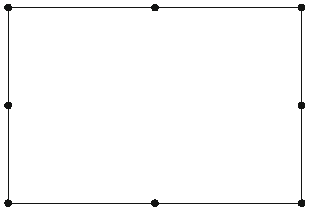
\includegraphics[width=0.86\linewidth]{figures/Chapter_03/Fig_3_06__PDFp111__Bookp099.pdf}
  \captionof{figure}{$Q_2^{(8)}$ 有限元.}\label{fig:taylor-hood-q2-8}
\end{elegantfigure}

Taylor--Hood 有限元空间对是不可压缩流方程离散中最常用的空间对之一,尤其是 $k=2$ 的情形.其广泛应用的一个原因是,与其他满足 inf-sup 条件的有限元空间对相比,$P_2/P_1$ 和 $Q_2/Q_1$ 的实现相对简单.注意,$P_1/P_0$ 和 $Q_1/Q_0$ 空间对已被证明不满足 inf-sup 条件,见例题\hyperref[ex:p1-p0-instability]{3.70} 和例题\hyperref[ex:q1-q0-instability]{3.71}.
\index{Taylor--Hood 有限元}

\end{note}

\begin{note}[Taylor--Hood 有限元的历史评述]\label{note:taylor-hood-history}
由于 Taylor--Hood 有限元空间对广受欢迎,早期已有不少工作试图证明其满足离散 inf-sup 条件.

\textcite{BercovierPironneau1979} 曾用不恰当的范数证明二维 $P_2/P_1$ 空间对满足如下离散 inf-sup 条件:
\begin{equation}\label{eq:taylor-hood-wrong-norm-infsup}
  \sup_{v^h\in V^h\setminus\{0\}}
      \frac{b(v^h,q^h)}{\|v^h\|_{L^2(\Omega)}}
  \ge C\|\nabla q^h\|_{L^2(\Omega)}
  \qquad\forall q^h\in Q^h.
\end{equation}
条件\cref{eq:taylor-hood-wrong-norm-infsup} 与离散 inf-sup 条件\cref{eq:discrete-infsup-condition} 的联系由 \textcite{GuzmanSalgadoSayas2013} 研究.

\textcite{BercovierPironneau1979} 的证明利用了一个估计:压力梯度的平方可由三角形内部边上的导数平方和估计,见该文估计式(2.11).这一估计要求每个三角形至少有两条内部边,因此当时假设每个三角形都含有一个不在边界 $\partial\Omega$ 上的顶点.\textcite{Verfurth1984} 以\cref{eq:taylor-hood-wrong-norm-infsup} 为基础,并利用定理\hyperref[thm:verfurth-continuous-pressure]{3.94} 中的判据,证明了正确的离散 inf-sup 条件\cref{eq:discrete-infsup-condition};其假设仍要求每个三角形至少有一个内部顶点.

随后,\textcite{Stenberg1990} 以及 \textcite{BrezziFalk1991} 证明了二维 $P_3/P_2$ 空间对满足离散 inf-sup 条件.Brezzi 和 Falk 的分析仍对有两条边位于区域边界上的三角形作了一个较弱的假设.最后,\textcite{Boffi1994} 给出了任意阶 $P_k/P_{k-1}$($k\ge2$)空间对的证明,不再对有两条边位于边界上的三角形作限制;该证明同样使用定理\hyperref[thm:verfurth-continuous-pressure]{3.94}.\textcite{MardalSchoberlWinther2013} 为二维 $P_2/P_1$ 空间对构造了 Fortin 算子.

三维 $P_2/P_1$ 空间对满足 inf-sup 条件的证明由 \textcite{Stenberg1987} 给出,随后 \textcite{Boffi1997} 将分析推广到高阶 Taylor--Hood 空间对.该分析要求每个四面体至少有一个顶点位于区域 $\Omega$ 内部.本节的叙述依据 \textcite[第 8.8.2 节]{Boffi2013} 和 \textcite{Boffi1994}.
\index{Taylor--Hood 有限元!历史}
\end{note}

\begin{lemma}[二维情形:三角剖分的必要条件]\label{lem:taylor-hood-two-triangles}
设 $\Omega\subset\mathbb{R}^2$ 是多边形区域,$\{\mathcal{T}^h\}$ 是由三角形构成的正则剖分族.若剖分中的三角形少于三个,则 $P_k/P_{k-1}$($k\ge2$)空间对不满足离散 inf-sup 条件\cref{eq:discrete-infsup-condition}.
\end{lemma}

\begin{proof}
分别讨论 $\mathcal{T}^h$ 由一个三角形和两个三角形组成的情形.

\textbf{$\mathcal{T}^h$ 由一个三角形组成.}由引理\ref{lem:inf-sup-condition},离散 inf-sup 条件等价于
\[
  \nabla\cdot V^h=Q^h,
\]
而这一等式又等价于以下两个包含关系同时成立:
\[
  \nabla\cdot V^h\subset Q^h,
  \qquad Q^h\subset\nabla\cdot V^h.
\]
先考虑参考单元 $\widehat K$,并设其顶点 $0$ 位于原点.在该顶点,$v^h\in V^h$ 的所有导数都由 $V^h$ 的齐次边界条件决定,因而均为零,特别是 $\nabla\cdot v^h(0)=0$.然而,任意 $q^h\in Q^h$ 在 $0$ 点的值不一定为零.因此,$Q^h\not\subset\nabla\cdot V^h$.

对一般网格单元 $K$,设顶点 $a_1$ 映到原点.由变换公式\hyperref[eq:appendix-b-27]{B.27} 或\hyperref[eq:appendix-b-31]{B.31} 可知
\[
  (\nabla\cdot v^h)(a_1)
  =\bigl(DF_K^{-1}(F_K(0))\bigr)^T
       :D_{\widehat x}\widehat v^h(0)=0,
\]
因为 $\widehat v^h$ 在原点的所有导数都为零.由同样的论证可得 $Q^h\not\subset\nabla\cdot V^h$.

\textbf{$\mathcal{T}^h$ 由两个三角形组成.}考虑\cref{fig:taylor-hood-two-triangles} 所示的情形.利用适当的仿射映射,可将一般情形中的 $K_1$ 和 $K_2$ 映到图示构形.为简化记号,仍将这两个三角形记作 $K_1$、$K_2$,并令 $\Omega=K_1\cup K_2$.

\begin{elegantfigure}[0.68\linewidth]
  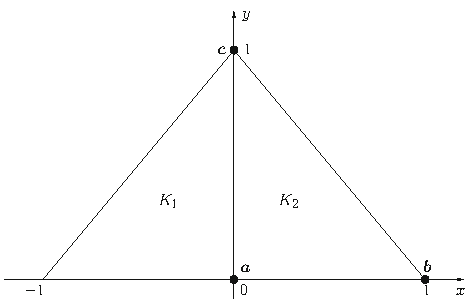
\includegraphics[width=0.90\linewidth]{figures/Chapter_03/Fig_3_07__PDFp112__Bookp100.pdf}
  \captionof{figure}{引理\ref{lem:taylor-hood-two-triangles} 的证明:两个三角形的情形.}\label{fig:taylor-hood-two-triangles}
\end{elegantfigure}

重心坐标见定义\hyperref[def:appendix-b-31]{B.31}.在图示坐标下,它们为
\begin{equation}\label{eq:taylor-hood-two-triangle-barycentric}
\begin{aligned}
  \lambda_{1,a}&=1+x-y, &\lambda_{1,c}&=y,\\
  \lambda_{2,a}&=1-x-y, &\lambda_{2,b}&=x, &\lambda_{2,c}&=y.
\end{aligned}
\end{equation}

令 $L(x)$ 为区间 $(0,1)$ 上关于权函数 $x(1-x)^3$ 的 $k-2$ 次 Legendre 多项式,也就是说,对所有次数 $l<k-2$ 的多项式 $p_l(x)$,有
\begin{equation}\label{eq:taylor-hood-weighted-orthogonality}
  \int_0^1x(1-x)^3L(x)p_l(x)\,\mathrm{d}x=0.
\end{equation}
利用 $L(x)$ 定义一个不依赖于 $y$ 的压力函数,并选取加法常数使其属于 $Q^h$,令其满足
\begin{equation}\label{eq:taylor-hood-pressure-derivative}
  \partial_xq^h(x)=
  \begin{cases}
    -L(-x),&x<0,\\
    L(x),&x\ge0.
  \end{cases}
\end{equation}
下面证明,这个压力函数在 $L^2(\Omega)$ 中正交于 $\nabla\cdot V^h$.

考察离散 inf-sup 条件\cref{eq:discrete-infsup-condition} 中的分子,并作分部积分,可得
\begin{equation}\label{eq:taylor-hood-orthogonality-integration}
  (\nabla\cdot v^h,q^h)
  =-(v^h,\nabla q^h)
  =-\int_{K_1\cup K_2}
       (v_1^h\partial_xq^h)(x)\,\mathrm{d}x.
\end{equation}
因此,只需考虑 $v^h$ 的第一个分量 $v_1^h$.由于 $v_1^h$ 属于 Taylor--Hood 空间,它满足以下性质:
\begin{itemize}
\item $v_1^h$ 在每个网格单元上都是 $k$ 次多项式.
\item 除了公共边以外,$v_1^h$ 在 $K_1$ 和 $K_2$ 的所有边上都为零.对每个网格单元,可将任意一个 $k-2$ 次多项式乘以相应的重心坐标(它们都是一次多项式),从而保证这一性质.
\item $v_1^h$ 在 $x=0$ 处连续.为满足这一性质,可将任意 $k-2$ 次多项式分解为一个关于 $y$ 的任意 $k-2$ 次多项式,以及一个在 $x=0$ 处为零的 $k-2$ 次多项式.
\end{itemize}
由此,$v_1^h$ 的一般形式为
\[
v_1^h(x)=
\begin{cases}
  \lambda_{1,a}\lambda_{1,c}
      \bigl(\widehat p_{k-2}(y)+x\widetilde p_{k-3}(x,y)\bigr),
      &x\in K_1,\\
  \lambda_{2,a}\lambda_{2,c}
      \bigl(\widehat p_{k-2}(y)+xp_{k-3}(x,y)\bigr),
      &x\in K_2,
\end{cases}
\]
其中,下标表示相应多项式的次数.将此表达式代入\cref{eq:taylor-hood-orthogonality-integration}.对 $K_1$ 上的积分使用\cref{eq:taylor-hood-pressure-derivative},作代换 $\xi=-x$,并利用重心坐标\cref{eq:taylor-hood-two-triangle-barycentric} 以及积分上下限的交换,可得
\[
\begin{aligned}
  &-\int_{K_1}\lambda_{1,a}\lambda_{1,c}
       \bigl(\widehat p_{k-2}(y)+x\widetilde p_{k-3}(x,y)\bigr)
       L(-x)\,\mathrm{d}x\\
  &=-\int_{-1}^{0}\int_0^{1+x}
       (1+x-y)y\bigl(\widehat p_{k-2}(y)
                  +x\widetilde p_{k-3}(x,y)\bigr)L(-x)\,\mathrm{d}y\,\mathrm{d}x\\
  &=\int_1^0\int_0^{1-\xi}
       (1-\xi-y)y\bigl(\widehat p_{k-2}(y)
                  -\xi\widetilde p_{k-3}(-\xi,y)\bigr)L(\xi)\,\mathrm{d}y\,\mathrm{d}\xi\\
  &=-\int_{K_2}\lambda_{2,a}\lambda_{2,c}
       \bigl(\widehat p_{k-2}(y)
                  -x\widetilde p_{k-3}(-x,y)\bigr)L(x)\,\mathrm{d}x.
\end{aligned}
\]
将该结果代入\cref{eq:taylor-hood-orthogonality-integration},含 $\widehat p_{k-2}(y)$ 的项相消,得到
\begin{equation}\label{eq:taylor-hood-orthogonality-final}
\begin{aligned}
  (\nabla\cdot v^h,q^h)
  &=-\int_{K_2}\lambda_{2,a}\lambda_{2,b}\lambda_{2,c}
       \bigl(p_{k-3}(x,y)-\widetilde p_{k-3}(-x,y)\bigr)L(x)\,\mathrm{d}x\\
  &=-\int_0^1xL(x)
       \left(\int_0^{1-x}(1-x-y)y\widetilde p_{k-3}(x,y)\,\mathrm{d}y\right)
       \mathrm{d}x.
\end{aligned}
\end{equation}
这里,$\widetilde p_{k-3}(x,y)$ 是一个 $k-3$ 次多项式.直接计算可知,对所有满足 $0\le i+j\le k-3$ 的 $i,j$,
\[
\begin{aligned}
  &\int_0^{1-x}(1-x-y)y x^iy^j\,\mathrm{d}y\\
  &=x^i\frac{(1-x)^{j+3}}{j+2}
       -x^i\frac{(1-x)^{j+3}}{j+3}\\
  &=(1-x)^3\frac{x^i(1-x)^j}{(j+2)(j+3)}\\
  &=(1-x)^3p_{k-3}(x),
\end{aligned}
\]
其中 $p_{k-3}(x)$ 是一个 $k-3$ 次多项式.将此结果代入\cref{eq:taylor-hood-orthogonality-final},再结合\cref{eq:taylor-hood-weighted-orthogonality},得到
\[
  (\nabla\cdot v^h,q^h)
  =-\int_0^1xL(x)(1-x)^3p_{k-3}(x)\,\mathrm{d}x=0.
\]
因此,离散 inf-sup 条件\cref{eq:discrete-infsup-condition} 不可能成立.
\end{proof}

\begin{lemma}[区域分解]\label{lem:domain-decomposition-infsup}
设 $\Omega=\Omega_1\cup\Omega_2$,并令
\[
  V^h(\Omega_i)=\{v^h\in V^h:\ v^h=0\text{ 于 }\Omega\setminus\Omega_i\},
  \qquad i=1,2.
\]
假设在两个子区域上分别成立离散 inf-sup 条件
\[
\begin{aligned}
  \sup_{v^h\in V^h(\Omega_1)\setminus\{0\}}
  \frac{\displaystyle\int_{\Omega_1}(\nabla\cdot v^h)q^h\,\mathrm{d}x}
       {\|\nabla v^h\|_{L^2(\Omega_1)}}
  \ge \beta_{1h}\|q^h\|_{L^2(\Omega_1)}
  \quad\forall q^h\in Q^h,\\
  \sup_{v^h\in V^h(\Omega_2)\setminus\{0\}}
  \frac{\displaystyle\int_{\Omega_2}(\nabla\cdot v^h)q^h\,\mathrm{d}x}
       {\|\nabla v^h\|_{L^2(\Omega_2)}}
  \ge \beta_{2h}\|q^h\|_{L^2(\Omega_2)}
  \quad\forall q^h\in Q^h.
\end{aligned}
\]
则整体区域上成立离散 inf-sup 条件
\begin{equation}\label{eq:domain-decomposition-global-infsup}
  \sup_{v^h\in V^h\setminus\{0\}}
  \frac{(\nabla\cdot v^h,q^h)}{\|\nabla v^h\|_{L^2(\Omega)}}
  \ge \beta_{\mathrm{ish}}\|q^h\|_{L^2(\Omega)}
  \qquad\forall q^h\in Q^h,
\end{equation}
其中 $\beta_{\mathrm{ish}}=\min\{\beta_{1h},\beta_{2h}\}/2$.若 $\Omega_1$ 与 $\Omega_2$ 不相交,则 $\beta_{\mathrm{ish}}=\min\{\beta_{1h},\beta_{2h}\}$.
\end{lemma}

\begin{proof}
任取 $q^h\in Q^h$.由子区域上的 inf-sup 条件以及引理\ref{lem:inf-sup-condition} 中的论证,可分别找到 $v_1^h\in V^h(\Omega_1)$ 和 $v_2^h\in V^h(\Omega_2)$,使得
\begin{equation}\label{eq:domain-decomposition-local-velocities}
\begin{aligned}
  \int_{\Omega_i}(\nabla\cdot v_i^h)q^h\,\mathrm{d}x
  &=\|q^h\|_{L^2(\Omega_i)}^2,\\
  \|\nabla v_i^h\|_{L^2(\Omega_i)}
  &\le \beta_{ih}^{-1}\|q^h\|_{L^2(\Omega_i)},
  \qquad i=1,2.
\end{aligned}
\end{equation}
令 $v^h=v_1^h+v_2^h\in V^h$.由\cref{eq:domain-decomposition-local-velocities} 第一式,
\begin{equation}\label{eq:domain-decomposition-numerator}
\begin{aligned}
  (\nabla\cdot v^h,q^h)
  &=\int_{\Omega_1}(\nabla\cdot v_1^h)q^h\,\mathrm{d}x
    +\int_{\Omega_2}(\nabla\cdot v_2^h)q^h\,\mathrm{d}x\\
  &=\|q^h\|_{L^2(\Omega_1)}^2+\|q^h\|_{L^2(\Omega_2)}^2
    \ge \|q^h\|_{L^2(\Omega)}^2.
\end{aligned}
\end{equation}
利用三角不等式、\cref{eq:domain-decomposition-local-velocities} 第二式,以及子区域上的压力范数不大于整体区域上的范数,得到
\begin{equation}\label{eq:domain-decomposition-gradient-bound}
\begin{aligned}
  \|\nabla v^h\|_{L^2(\Omega)}
  &\le \|\nabla v_1^h\|_{L^2(\Omega_1)}
       +\|\nabla v_2^h\|_{L^2(\Omega_2)}\\
  &\le \beta_{1h}^{-1}\|q^h\|_{L^2(\Omega_1)}
       +\beta_{2h}^{-1}\|q^h\|_{L^2(\Omega_2)}\\
  &\le \max\left\{\frac{1}{\beta_{1h}},\frac{1}{\beta_{2h}}\right\}
       \left(\|q^h\|_{L^2(\Omega_1)}+\|q^h\|_{L^2(\Omega_2)}\right)\\
  &\le \frac{2}{\min\{\beta_{1h},\beta_{2h}\}}
       \|q^h\|_{L^2(\Omega)}.
\end{aligned}
\end{equation}
将\cref{eq:domain-decomposition-numerator,eq:domain-decomposition-gradient-bound} 合并可知,对每个 $q^h\in Q^h$,都存在 $v^h\in V^h$ 使得
\begin{equation}\label{eq:domain-decomposition-ratio}
  \frac{(\nabla\cdot v^h,q^h)}{\|\nabla v^h\|_{L^2(\Omega)}}
  \ge \frac{1}{2}\min\{\beta_{1h},\beta_{2h}\}
       \|q^h\|_{L^2(\Omega)}.
\end{equation}
对\cref{eq:domain-decomposition-ratio} 两边关于 $V^h$ 取上确界,即得\cref{eq:domain-decomposition-global-infsup}.

若两个子区域不相交,则梯度范数的平方满足
\[
\begin{aligned}
  \|\nabla v^h\|_{L^2(\Omega)}^2
  &=\|\nabla v_1^h\|_{L^2(\Omega_1)}^2
    +\|\nabla v_2^h\|_{L^2(\Omega_2)}^2\\
  &\le \beta_{1h}^{-2}\|q^h\|_{L^2(\Omega_1)}^2
       +\beta_{2h}^{-2}\|q^h\|_{L^2(\Omega_2)}^2\\
  &\le \max\{\beta_{1h}^{-2},\beta_{2h}^{-2}\}
       \left(\|q^h\|_{L^2(\Omega_1)}^2
             +\|q^h\|_{L^2(\Omega_2)}^2\right)\\
  &= \min\{\beta_{1h},\beta_{2h}\}^{-2}
       \|q^h\|_{L^2(\Omega)}^2.
\end{aligned}
\]
取平方根,再按上述推理即可得到引理的最后一个结论.
\end{proof}

\begin{note}[子区域多于两个时]\label{note:domain-decomposition-many-subdomains}
若将 $\Omega$ 分解为两个以上的子区域,也可证明与\hyperref[lem:domain-decomposition-infsup]{引理~\ref{lem:domain-decomposition-infsup}} 类似的结论.估计\cref{eq:domain-decomposition-numerator} 的推导不变;在估计\cref{eq:domain-decomposition-gradient-bound} 中,会出现一个较大的因子,该因子取决于子区域相互重叠的次数.因此,相应整体 inf-sup 条件中的常数会较小.

证明 Taylor--Hood 空间对 $P_k/P_{k-1}$($k\ge2$)满足离散 inf-sup 条件时,首先将三角剖分分解为由三个相邻三角形组成的宏单元.\textcite[第 499 页]{Boffi2013} 指出,每个多边形区域的三角剖分都可以表示为若干互不相交的三角形三元组,以及若干个由三元组并成、且至多有三处相交的多边形的并.因此,对估计\cref{eq:domain-decomposition-gradient-bound} 中常数有影响的最大重叠数与剖分无关,整体 inf-sup 常数的缩放因子也就与剖分无关.
\index{Taylor--Hood 有限元!宏单元分解}
\end{note}

\begin{theorem}[二维情形:剖分的充分条件]\label{thm:taylor-hood-2d-sufficient}
设 $\Omega\subset\mathbb{R}^2$ 是多边形区域,$\{\mathcal{T}^h\}$ 是由三角形构成的正则剖分族.若剖分至少含有三个三角形,则 $P_k/P_{k-1}$($k\ge2$)空间对满足离散 inf-sup 条件\cref{eq:discrete-infsup-condition}.
\end{theorem}

\begin{proof}
取准一致剖分族中的任意一个剖分 $\mathcal{T}^h$.由\hyperref[lem:domain-decomposition-infsup]{引理~\ref{lem:domain-decomposition-infsup}} 和\cref{note:domain-decomposition-many-subdomains},只需证明任意一组三个三角形上的离散 inf-sup 条件.

取 $\mathcal{T}^h$ 中任意一个三角形 $K_2$,令其相邻三角形为 $K_1$ 和 $K_3$.通过参考映射 $F_{K_2}^{-1}$ 将三角形映射,使 $K_2$ 成为参考三角形,见\cref{fig:taylor-hood-three-triangles}.为简化记号,仍以 $K_1,K_2,K_3$ 表示映射后的三角形,并令 $\Omega=K_1\cup K_2\cup K_3$.

\begin{elegantfigure}[0.9\linewidth]
  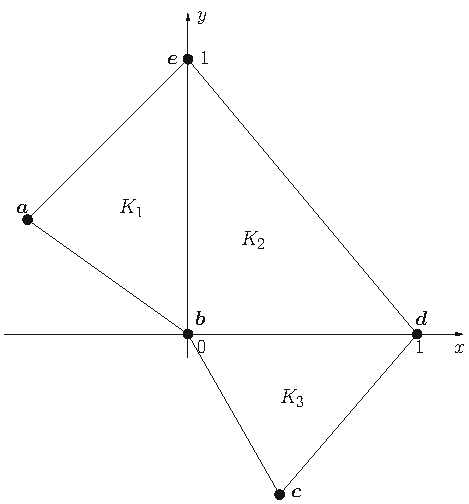
\includegraphics[width=0.9\linewidth]{figures/Chapter_03/Fig_3_08__PDFp117__Bookp105.pdf}
  \captionof{figure}{定理\ref{thm:taylor-hood-2d-sufficient} 的证明:三个三角形的构形.}\label{fig:taylor-hood-three-triangles}
\end{elegantfigure}

证明 $V^h=V^h(\Omega)$ 与 $Q^h=Q^h(\Omega)$ 满足离散 inf-sup 条件的主要思路,是应用\thmref{thm:verfurth-continuous-pressure} 中的判据.为此,只需验证\corref{cor:continuous-pressure-gradient-infsup} 给出的条件.证明采用归纳法,从 $k=2$ 开始.

\textbf{预备工作.}在网格单元 $K_1$ 上,记在边 $E_{a,b}$ 上为零的重心坐标为 $\lambda_{1,a,b}$,其他重心坐标也作类似记号.令 $L_{1,l,x}(x)$ 表示区间 $[x_a,0]$ 上关于测度 $\mathrm{d}\mu_{1,x}$ 的 $l$ 次 Legendre 多项式,其中 $x_a$ 是顶点 $a$ 的 $x$ 坐标,测度定义为
\[
\begin{aligned}
  \int_{x_a}^{0} f(x)\,\mathrm{d}\mu_{1,x}
  &=\int_{K_1}\lambda_{1,a,b}(x,y)\lambda_{1,a,e}(x,y)f(x)
       \,\mathrm{d}x\,\mathrm{d}y,\\
  &\qquad \forall f:[x_a,0]\to\mathbb{R}.
\end{aligned}
\]
该 Legendre 多项式满足
\begin{equation}\label{eq:taylor-hood-legendre-orthogonality}
\begin{aligned}
  0&=\int_{x_a}^{0}L_{1,l,x}(x)p_k(x)\,\mathrm{d}\mu_{1,x}\\
   &=\int_{K_1}\lambda_{1,a,b}\lambda_{1,a,e}
       L_{1,l,x}(x)p_k(x)\,\mathrm{d}x\,\mathrm{d}y,\\
  &\qquad \forall p_k\text{ 且 }\deg p_k<l.
\end{aligned}
\end{equation}
类似地,定义 $L_{2,l,x}(x)$(使用 $\lambda_{2,d,e},\lambda_{2,b,d}$)、$L_{2,l,y}(y)$(使用 $\lambda_{2,d,e},\lambda_{2,b,e}$)以及 $L_{3,l,y}(y)$(使用 $\lambda_{3,b,c},\lambda_{3,c,d}$).所有 Legendre 多项式均作归一化,使其在自变量为 $0$ 时取值为 $1$.

\textbf{归纳起始:$k=2$ 的情形.}任取 $q^h\in Q^h$,逐个三角形定义函数 $v^h=((v_1^h),(v_2^h))^T$:
\[
v_1^h(x,y)=
\begin{cases}
 -\lambda_{1,a,b}\lambda_{1,a,e}\|\nabla q^h\|_{L^2(\Omega)}\sigma,&(x,y)\in K_1,\\
 \begin{aligned}
  -\lambda_{2,d,e}\lambda_{2,b,d}\|\nabla q^h\|_{L^2(\Omega)}\sigma\\[-.25em]
  -\lambda_{2,d,e}\lambda_{2,b,e}\partial_xq^h,
 \end{aligned}&(x,y)\in K_2,\\
 -\lambda_{3,b,c}\lambda_{3,c,d}\partial_xq^h,&(x,y)\in K_3,
\end{cases}
\]
\[
v_2^h(x,y)=
\begin{cases}
 -\lambda_{1,a,b}\lambda_{1,a,e}\partial_yq^h,&(x,y)\in K_1,\\
 \begin{aligned}
  -\lambda_{2,d,e}\lambda_{2,b,e}\|\nabla q^h\|_{L^2(\Omega)}\tau\\[-.25em]
  -\lambda_{2,d,e}\lambda_{2,b,d}\partial_yq^h,
 \end{aligned}&(x,y)\in K_2,\\
 -\lambda_{3,b,c}\lambda_{3,c,d}\|\nabla q^h\|_{L^2(\Omega)}\tau,&(x,y)\in K_3.
\end{cases}
\]
选取 $\sigma,\tau\in\{-1,1\}$,使得下列量非负:
\[
\begin{aligned}
  \sigma_1&=\sigma\|\nabla q^h\|_{L^2(\Omega)}\Bigl(
       \int_{K_1}\lambda_{1,a,b}\lambda_{1,a,e}\partial_xq^h\,\mathrm{d}x\\
       &\qquad+\int_{K_2}\lambda_{2,d,e}\lambda_{2,b,d}\partial_xq^h\,\mathrm{d}x\Bigr),\\
  \tau_1&=\tau\|\nabla q^h\|_{L^2(\Omega)}\Bigl(
       \int_{K_2}\lambda_{2,d,e}\lambda_{2,b,e}\partial_yq^h\,\mathrm{d}x\\
       &\qquad+\int_{K_3}\lambda_{3,b,c}\lambda_{3,c,d}\partial_yq^h\,\mathrm{d}x\Bigr).
\end{aligned}
\]

下面验证 $v^h\in V^h$.首先,在每个网格单元上,$v^h$ 的每一项都是两个重心坐标(一次多项式)与常数因子的乘积,因此 $v^h$ 在各网格单元上至多为二次多项式.其次,由于定义中包含在 $\partial\Omega$ 上为零的相应重心坐标,$v^h$ 在 $\partial\Omega$ 上为零.最后,$v^h$ 在边 $E_{b,e}$ 和 $E_{b,d}$ 上连续.以 $E_{b,e}$ 为例,在该边上有 $\lambda_{1,a,e}=\lambda_{2,d,e}$、$\lambda_{1,a,b}=\lambda_{2,b,d}$;此外,$q^h$ 连续,故其切向导数 $\partial_xq^h$ 也连续.因此 $v^h$ 在 $E_{b,e}$ 上连续.对 $E_{b,d}$ 可作类似论证.

现在证明\cref{eq:continuous-pressure-gradient-test} 中关于速度范数的相应估计.利用重心坐标的取值均在 $[0,1]$ 内以及三角不等式,得到
\begin{equation}\label{eq:taylor-hood-k2-velocity-bound}
\begin{aligned}
  \|v^h\|_{L^2(\Omega)}^2
  &=\int_{K_1}\bigl((v_1^h)^2+(v_2^h)^2\bigr)\,\mathrm{d}x\\
  &\quad+\int_{K_2}\bigl((v_1^h)^2+(v_2^h)^2\bigr)\,\mathrm{d}x\\
  &\quad+\int_{K_3}\bigl((v_1^h)^2+(v_2^h)^2\bigr)\,\mathrm{d}x\\
  &\le \int_{K_1}\left(\|\nabla q^h\|_{L^2(\Omega)}^2
                        +(\partial_yq^h)^2\right)\,\mathrm{d}x\\
  &\quad+2\int_{K_2}\left(2\|\nabla q^h\|_{L^2(\Omega)}^2
                        +(\partial_xq^h)^2+(\partial_yq^h)^2\right)\,\mathrm{d}x\\
  &\quad+\int_{K_3}\left((\partial_xq^h)^2
                        +\|\nabla q^h\|_{L^2(\Omega)}^2\right)\,\mathrm{d}x\\
  &\le C\Bigl(|\Omega|\|\nabla q^h\|_{L^2(\Omega)}^2
       +\|\nabla q^h\|_{L^2(K_1)}^2+\|\nabla q^h\|_{L^2(K_2)}^2\\
       &\qquad+\|\nabla q^h\|_{L^2(K_3)}^2\Bigr)\\
  &\le C_2\|\nabla q^h\|_{L^2(\Omega)}^2.
\end{aligned}
\end{equation}
由此可见,常数 $C_2$ 与 $q^h$ 和 $v^h$ 均无关.

为证\cref{eq:continuous-pressure-gradient-test} 中关于双线性型的另一个不等式,先证明若 $b(v^h,q^h)=0$,则 $\nabla q^h=0$.直接计算可得
\begin{equation}\label{eq:taylor-hood-k2-kernel-identity}
\begin{aligned}
  0=-b(v^h,q^h)
  &=\int_\Omega(\nabla\cdot v^h)q^h\,\mathrm{d}x
   =-\int_\Omega v^h\cdot\nabla q^h\,\mathrm{d}x\\
  &=\int_{K_1}\lambda_{1,a,b}\lambda_{1,a,e}(\partial_yq^h)^2\,\mathrm{d}x+\sigma_1\\
  &\quad+\int_{K_2}\lambda_{2,d,e}\lambda_{2,b,e}(\partial_xq^h)^2\,\mathrm{d}x\\
  &\quad+\int_{K_2}\lambda_{2,d,e}\lambda_{2,b,d}(\partial_yq^h)^2\,\mathrm{d}x\\
  &\quad+\tau_1+\int_{K_3}\lambda_{3,b,c}\lambda_{3,c,d}(\partial_xq^h)^2\,\mathrm{d}x.
\end{aligned}
\end{equation}
由于重心坐标在网格单元内部为正,且 $\sigma_1,\tau_1$ 均非负,上式中的每一项都必须为零.因此,立即得到 $\partial_yq^h=0$ 于 $K_1$,$\partial_xq^h=\partial_yq^h=0$ 于 $K_2$,以及 $\partial_xq^h=0$ 于 $K_3$.再由 $\sigma_1=0$ 及 $\partial_xq^h=0$ 于 $K_2$,可得 $\partial_xq^h=0$ 于 $K_1$;同理可得 $\partial_yq^h=0$ 于 $K_3$.综上,$\nabla q^h=0$ 于 $\Omega$,故存在常数 $C_1(q^h)>0$,使得
\[
  -b(v^h,q^h)\ge C_1(q^h)\|\nabla q^h\|_{L^2(\Omega)}^2.
\]
将 $v^h$ 换为 $-v^h$,便得到\cref{eq:continuous-pressure-gradient-test} 所需的双线性型下界.
还需证明可选取一个与 $q^h$ 无关的正数 $C_1$.首先注意,对任意 $\alpha\in\mathbb{R}\setminus\{0\}$,将函数换成 $\alpha q^h$ 并相应地将速度换成 $\alpha v^h$,所得估计中的常数仍为 $C_1(q^h)$.因此,$C_1(q^h)$ 在球面
\[
  S_q=\{q^h\in Q^h:\ \|q^h\|_{L^2(\Omega)}=q>0\}
\]
上取遍所有可能的值.由于 $Q^h$ 是有限维空间,$S_q$ 是紧集.

另一方面,任取固定的 $\widetilde q^h\in Q^h$,考虑 $q_\varepsilon^h=q^h+\varepsilon\widetilde q^h$,并以同样方式定义 $v_\varepsilon^h$,即可得到常数 $C_1(q_\varepsilon^h)$.当 $\varepsilon\to0$ 时,$q_\varepsilon^h\to q^h$;由范数的连续性以及微分的线性性,$v_\varepsilon^h\to v^h$.由积分的线性性和范数的连续性可知
\[
\begin{aligned}
\lim_{\varepsilon\to0}
  \frac{-b(v_\varepsilon^h,q_\varepsilon^h)}
       {\|\nabla q_\varepsilon^h\|_{L^2(\Omega)}^2}
 &=\lim_{\varepsilon\to0}
  \frac{-\int_\Omega v_\varepsilon^h\cdot\nabla q^h\,\mathrm{d}x}
       {\|\nabla q_\varepsilon^h\|_{L^2(\Omega)}^2}\\
 &\quad-\lim_{\varepsilon\to0}
  \frac{\varepsilon\int_\Omega v_\varepsilon^h\cdot\nabla\widetilde q^h\,\mathrm{d}x}
       {\|\nabla q_\varepsilon^h\|_{L^2(\Omega)}^2}\\
 &=\frac{-\int_\Omega v^h\cdot\nabla q^h\,\mathrm{d}x}
       {\|\nabla q^h\|_{L^2(\Omega)}^2}
 \ge C_1(q^h).
\end{aligned}
\]
因此可令 $C_1(q_\varepsilon^h)\to C_1(q^h)$,从而可将 $C_1(q^h)$ 选为关于 $q^h$ 连续的函数.由于 $C_1(q^h)$ 在 $S_q$ 上连续,且 $S_q$ 紧,由 Weierstrass 定理可知 $C_1(q^h)$ 能取到其下确界,且下确界就是其最小值.由于 $C_1(q^h)$ 的取值均为正数,故
\[
  C_1=\inf_{q^h\in S_q}C_1(q^h)
     =\min_{q^h\in S_q}C_1(q^h)>0
\]
是满足\cref{eq:continuous-pressure-gradient-test} 第一条不等式的正数,且与 $q^h$ 无关.

以上分析是在\cref{fig:taylor-hood-three-triangles} 所示的参考构形上进行的,因此 $C_1$ 与网格尺度无关.将该构形变换到区域 $\Omega$ 中,需要分别变换离散 inf-sup 条件的分子和分母.变换分子会产生因子 $|\det(B_K)|^{-1}$,其中 $B_K$ 是仿射变换的矩阵,见\hyperref[eq:appendix-b-35]{B.35}.分母中的两个范数各产生因子 $|\det(B_K)|^{-1/2}$,见\hyperref[eq:appendix-b-32]{B.32} 和\hyperref[eq:appendix-b-34]{B.34}.因此这些因子相消,$\Omega$ 中该构形的 inf-sup 常数与网格尺度无关.

\textbf{归纳步骤:$k>2$ 的情形.}归纳假设:\thmref{thm:taylor-hood-2d-sufficient} 对 $P_{k-1}/P_{k-2}$ 已成立.再次任取 $q^h\in Q^h$.假设至少有一个三角形上 $q^h$ 的次数恰为 $k-1$;否则,结论由归纳假设直接得到.按 $k=2$ 时的相同思路定义相应的 $v^h$:
\[
v_1^h(x,y)=
\begin{cases}
 -\lambda_{1,a,b}\lambda_{1,a,e}\|\nabla q^h\|_{L^2(\Omega)}L_{1,k-2,x}(x)\sigma,&(x,y)\in K_1,\\
 \begin{aligned}
  -\lambda_{2,d,e}\lambda_{2,b,d}\|\nabla q^h\|_{L^2(\Omega)}L_{2,k-2,x}(x)\sigma\\[-.25em]
  -\lambda_{2,d,e}\lambda_{2,b,e}\partial_xq^h,
 \end{aligned}&(x,y)\in K_2,\\
 -\lambda_{3,b,c}\lambda_{3,c,d}\partial_xq^h,&(x,y)\in K_3,
\end{cases}
\]
\[
v_2^h(x,y)=
\begin{cases}
 -\lambda_{1,a,b}\lambda_{1,a,e}\partial_yq^h,&(x,y)\in K_1,\\
 \begin{aligned}
  -\lambda_{2,d,e}\lambda_{2,b,e}\|\nabla q^h\|_{L^2(\Omega)}L_{2,k-2,y}(y)\tau\\[-.25em]
  -\lambda_{2,d,e}\lambda_{2,b,d}\partial_yq^h,
 \end{aligned}&(x,y)\in K_2,\\
 -\lambda_{3,b,c}\lambda_{3,c,d}\|\nabla q^h\|_{L^2(\Omega)}L_{3,k-2,y}(y)\tau,&(x,y)\in K_3.
\end{cases}
\]
选取 $\sigma,\tau\in\{-1,1\}$,使得下列两项非负:
\[
\begin{aligned}
  \sigma_1&=\sigma\|\nabla q^h\|_{L^2(\Omega)}\Bigl(
       \int_{K_1}\lambda_{1,a,b}\lambda_{1,a,e}L_{1,k-2,x}\partial_xq^h\,\mathrm{d}x\\
       &\qquad+\int_{K_2}\lambda_{2,d,e}\lambda_{2,b,d}L_{2,k-2,x}\partial_xq^h\,\mathrm{d}x\Bigr),\\
  \tau_1&=\tau\|\nabla q^h\|_{L^2(\Omega)}\Bigl(
       \int_{K_2}\lambda_{2,d,e}\lambda_{2,b,e}L_{2,k-2,y}\partial_yq^h\,\mathrm{d}x\\
       &\qquad+\int_{K_3}\lambda_{3,b,c}\lambda_{3,c,d}L_{3,k-2,y}\partial_yq^h\,\mathrm{d}x\Bigr).
\end{aligned}
\]
利用与 $k=2$ 情形相同的论证,可以证明 $v^h\in V^h$.还需补充两点:其一,Legendre 多项式的次数为 $k-2$,重心坐标的次数为 $1$,所以 $v^h$ 在每个网格单元上的次数至多为 $k$;其二,由归一化方式可知,$L_{1,k-2,x}$ 与 $L_{2,k-2,x}$ 在 $x=0$ 处取值相同,$L_{2,k-2,y}$ 与 $L_{3,k-2,y}$ 在 $y=0$ 处取值相同,这保证了 $v^h$ 的连续性.

证明\cref{eq:continuous-pressure-gradient-test} 中第二个估计的方式与\cref{eq:taylor-hood-k2-velocity-bound} 相同;此外只需用到 Legendre 多项式有界,且这些界与 $q^h,v^h$ 无关.现在假设 $b(v^h,q^h)=0$.作与\cref{eq:taylor-hood-k2-kernel-identity} 类似的计算,并使用 $k=2$ 时相同的论证,可得 $\partial_yq^h=0$ 于 $K_1$,$\partial_xq^h=\partial_yq^h=0$ 于 $K_2$,$\partial_xq^h=0$ 于 $K_3$,且 $\sigma_1=\tau_1=0$.由 $\sigma_1=0$ 以及 $\partial_xq^h=0$ 于 $K_2$,得到
\[
  \int_{K_1}\lambda_{1,a,b}\lambda_{1,a,e}
       L_{1,k-2,x}(x)\partial_xq^h\,\mathrm{d}x=0.
\]
由正交性\cref{eq:taylor-hood-legendre-orthogonality} 可知,$\partial_xq^h$ 在 $K_1$ 上是次数小于 $k-2$ 的多项式.因此,$q^h$ 在 $K_1$ 上的次数小于 $k-1$.同理,$q^h$ 在 $K_3$ 上的次数也小于 $k-1$.综上,$q^h$ 在每个网格单元上的次数均小于 $k-1$,这与假设矛盾.因此存在常数 $C_1(q^h)>0$,使得
\[
  -b(v^h,q^h)\ge C_1(q^h)\|\nabla q^h\|_{L^2(\Omega)}^2.
\]
同样将 $v^h$ 换为 $-v^h$,即可得到\cref{eq:continuous-pressure-gradient-test} 所需的双线性型下界.
选取与 $q^h$ 及网格尺度无关的 $C_1$ 的论证与 $k=2$ 时相同.至此定理得证.
\end{proof}

\begin{theorem}[三维情形]\label{thm:taylor-hood-3d}
设 $\Omega\subset\mathbb{R}^3$ 是多面体区域,$\{\mathcal{T}^h\}$ 是由四面体构成的正则剖分族.假设每个四面体至少有一个顶点位于 $\Omega$ 内部,则 $P_k/P_{k-1}$($k\ge2$)空间对满足离散 inf-sup 条件\cref{eq:discrete-infsup-condition}.
\end{theorem}

\begin{proof}
证明使用\cref{subsec:macroelement-techniques} 中介绍的宏单元方法.

考虑 $\mathcal{T}^h$ 的一个重叠宏单元划分,并对 $\Omega$ 内部的每个顶点 $a$ 定义宏单元
\[
  M_a=\{K:\ K\in\mathcal{T}^h,\ a\text{ 是 }K\text{ 的顶点}\}.
\]
由于剖分族正则,具有共同顶点的四面体数存在一致上界.因此,宏单元类型只有有限种.由每个四面体至少有一个内部顶点的假设可知,每个四面体至少属于一个宏单元;而每个网格单元至多属于四个宏单元.因此,\hyperref[lem:macroelement-velocity-1]{引理~\ref{lem:macroelement-velocity-1}} 和\cref{note:macroelement-overlap} 的几何假设均成立.剩下只需验证宏单元条件\cref{eq:macroelement-condition}.

任取 $K\in M_a$,并令 $E$ 为 $K$ 的一条以 $a$ 为端点的边.选择坐标系,使 $E$ 位于 $x$ 轴上.任取
\[
  q^h\in Q_{\mathrm{grad},M_a}^h\cap Q_{0,M_a}^h.
\]
先证明 $q^h$ 在 $K$ 上为常数.为此定义函数 $v^h$:对 $M_a$ 中所有与边 $E$ 相邻的网格单元 $K_i$,令
\[
  v^h=\bigl(-\lambda_{i,1}\lambda_{i,2}\partial_xq^h,\ 0,\ 0\bigr)^T
  \quad\text{于 }K_i,
\]
其中,$\lambda_{i,1}$ 和 $\lambda_{i,2}$ 是 $K_i$ 中分别对应于不含公共边 $E$ 的两个面的重心坐标.在 $M_a$ 中其他网格单元上,令 $v^h=0$.下面验证 $v^h\in V_{0,M_a}^h$.首先,$\partial_xq^h$ 是 $k-2$ 次多项式,而 $\lambda_{i,1},\lambda_{i,2}$ 都是一次多项式,所以 $v^h$ 是 $k$ 次多项式.其次,由所选重心坐标的构造可知,$v^h|_{\partial M_a}=0$.最后,由于 $q^h$ 连续,其在各面上的切向导数也连续;边 $E$ 是所有含该边的面上的切向量,故 $\partial_xq^h$ 在这些面上连续.重心坐标在这些面上也连续,而 $v^h$ 在其他面上为零.因此 $v^h$ 连续,确有 $v^h\in V_{0,M_a}^h$.

由于 $q^h\in Q_{\mathrm{grad},M_a}^h$,有
\[
\begin{aligned}
  0&=(\nabla\cdot v^h,q^h)_{M_a}
    =-\int_{M_a}v^h\cdot\nabla q^h\,\mathrm{d}x\\
   &=\sum_{K_i\in M_a:\,K_i\supset E}
       \int_{K_i}\lambda_{i,1}\lambda_{i,2}
              (\partial_xq^h)^2\,\mathrm{d}x.
\end{aligned}
\]
因此 $\partial_xq^h=0$,从而 $q^h$ 在每个这样的 $K_i$ 上都与 $x$ 无关,特别是在 $K$ 上如此.对 $K$ 中以 $a$ 为端点的另外两条边重复上述论证,可知 $q^h$ 在 $K$ 上沿三个线性无关方向的偏导数均为零,故 $\nabla q^h=0$ 于 $K$.

对 $M_a$ 中每个 $K$ 重复上述过程,可知 $q^h$ 在每个网格单元上均为常数.由于 $q^h$ 连续,它在整个 $M_a$ 上为常数.$Q_{0,M_a}^h$ 中唯一的常数函数是零,故 $q^h=0$,这正是宏单元条件\cref{eq:macroelement-condition}.
\end{proof}

\begin{note}[$Q_k/Q_{k-1}$($k\ge2$)空间对]\label{note:qk-qkminus1-stability}
二维情形下 $Q_2/Q_1$ 空间对满足离散 inf-sup 条件\cref{eq:discrete-infsup-condition},由\textcite{Stenberg1984} 使用其文中提出的宏单元方法证明;该宏单元由两个网格单元组成.随后,\textcite{Stenberg1990} 将分析推广到高阶 $Q_k/Q_{k-1}$ 空间对.三维情形下 $Q_2/Q_1$ 空间对的离散 inf-sup 条件由\textcite{Stenberg1987} 证明.
\index{$Q_k/Q_{k-1}$ 空间对}
\end{note}

\begin{note}[修改的 Taylor--Hood 有限元]\label{note:modified-taylor-hood}
设三角剖分 $\mathcal{T}^h$ 由三角形、四边形或六面体构成,并对这些网格单元作正则加密,例如将三角形的各边中点相连,得到剖分 $\mathcal{T}^{h/2}$.

为简明起见,只讨论三角形.修改的 Taylor--Hood 有限元空间取细网格上的 $P_1^{h/2}$ 作为速度空间,取粗网格上的 $P_1^h$ 作为压力空间.细网格 $P_1^{h/2}$ 的自由度数与粗网格空间 $P_2^h$ 相同,但此处采用的是分片线性函数,而非分片二次函数.四边形和六面体也可作类似构造.若已有程序只支持最低阶有限元,这种修改的 Taylor--Hood 空间便可能有用.

修改的 Taylor--Hood 空间对满足离散 inf-sup 条件的性质,例如可用\cref{note:taylor-hood-history} 中提到的 Bercovier--Pironneau(1979)和 Verfürth(1984)的方法证明.
\index{Taylor--Hood 有限元!修改的 Taylor--Hood 有限元}
\end{note}

\subsection{单纯形网格上的不连续压力空间}\label{sec:scott-vogelius}

\begin{note}[动机]\label{note:discontinuous-pressure-motivation}
文献中采用不连续压力有限元空间(finite element spaces with discontinuous pressure)的一个动机,是这类空间具有局部质量守恒(local mass conservation)性质.关于这一点,见笔记\hyperref[note:stokes-local-mass-conservation-discontinuous-pressure]{4.32}.
\index{不连续压力!局部质量守恒}
\end{note}

\begin{note}[构造的基本思路]\label{note:discontinuous-pressure-construction}
在单纯形网格上采用不连续压力逼近的空间对包括:\textcite{CrouzeixRaviart1973} 提出的 $P_2^{\mathrm{bubble}}/P_1^{\mathrm{disc}}$ 空间对;\textcite{ScottVogelius1985} 引入的 Scott--Vogelius 空间对 $P_k/P_{k-1}^{\mathrm{disc}}$($k\ge2$);以及\textcite{BernardiRaugel1985} 提出的 Bernardi--Raugel 空间.例题\hyperref[ex:p1-p0-instability]{3.70} 和\hyperref[ex:scott-vogelius-macroelement]{3.73} 已经说明,采用 $P_k/P_{k-1}^{\mathrm{disc}}$ 组合通常会违反离散 inf-sup 条件\cref{eq:discrete-infsup-condition}.

Scott--Vogelius 有限元仍采用 $P_k/P_{k-1}^{\mathrm{disc}}$($k\ge2$),但只在能够证明离散 inf-sup 条件成立的特殊网格上使用.$P_2^{\mathrm{bubble}}/P_1^{\mathrm{disc}}$ 有限元和 Bernardi--Raugel 有限元的基本思路,则是向离散速度空间加入气泡函数,直至速度空间足够大,从而满足离散 inf-sup 条件;参见笔记\hyperref[note:infsup-not-inherited]{3.52}.
\index{Scott--Vogelius 有限元}
\index{Bernardi--Raugel 有限元}
\end{note}

\begin{note}[Scott--Vogelius 有限元空间对]\label{note:scott-vogelius-pair}
该空间对为 $P_k/P_{k-1}^{\mathrm{disc}}$($k\ge2$).由于
\[
  \nabla\cdot V^h\subseteq \nabla\cdot P_k
      =P_{k-1}^{\mathrm{disc}}=Q^h,
\]
这一空间对中的有限元速度是弱无散的,这是一个理想性质.不过,正如例题\hyperref[ex:scott-vogelius-macroelement]{3.73} 已经说明的,Scott--Vogelius 有限元通常不满足离散 inf-sup 条件\cref{eq:discrete-infsup-condition}.但在某些特殊情形,也就是特殊网格上,可以证明 $P_k/P_{k-1}^{\mathrm{disc}}$ 空间对满足离散 inf-sup 条件.本节将概述已知结果.
\index{Scott--Vogelius 有限元!弱无散性}
\end{note}

\begin{note}[$P_k/P_{k-1}^{\mathrm{disc}}$ 空间对的二维情形]\label{note:scott-vogelius-2d}
\textcite{ScottVogelius1985} 已证明,在二维情形下,只要网格中没有所谓的奇异顶点(singular vertex),$k\ge4$ 时 $P_k/P_{k-1}^{\mathrm{disc}}$ 空间对满足离散 inf-sup 条件\cref{eq:discrete-infsup-condition}.若一个内部顶点处相交的网格边落在两条直线上,就称该顶点为奇异顶点.关于离散 inf-sup 条件普遍成立的反例正是采用了奇异顶点,见\cref{fig:scott-vogelius-macroelement}.

解决这一问题的基本思路是采用不含奇异顶点的网格,为此构造所谓的重心加密网格(barycentric-refined mesh).从任意一个可容许的三角剖分出发,将每个网格单元的所有顶点与该单元的重心相连,即可引入新的网格边.这样便把单元细分为更小的三角形,\cref{fig:barycentric-refinement} 给出了一个例子.\textcite{Qin1994} 证明,在重心加密网格上,$k\in\{2,3\}$ 时 $P_k/P_{k-1}^{\mathrm{disc}}$ 空间对满足离散 inf-sup 条件;$k=2$ 的证明也见例题\hyperref[ex:barycentric-refinement-scott-vogelius]{4.144}.注意,$k\ge4$ 的情形已由\textcite{ScottVogelius1985} 的分析涵盖.

在文献中,重心加密网格上的 $P_2/P_1^{\mathrm{disc}}$ 空间对偶尔会被采用,尤其用于展示具有弱无散速度解的空间对的优点,例如参见 John et al.(2015)及其中的参考文献.
\index{奇异顶点}
\index{重心加密网格}
\end{note}

\begin{note}[$P_k/P_{k-1}^{\mathrm{disc}}$ 空间对的三维情形]\label{note:scott-vogelius-3d}
在三维情形下,采用重心加密网格可以避免奇异顶点和奇异边.\textcite{Zhang2005} 已证明,在这类网格上,$k\le3$ 时 $P_k/P_{k-1}^{\mathrm{disc}}$ 空间对满足离散 inf-sup 条件.证明使用了\textcite{Stenberg1984} 的宏单元方法,即第\hyperref[subsec:macroelement-techniques]{3.5.4 节} 介绍的方法.

\begin{elegantfigure}[0.9\linewidth]
  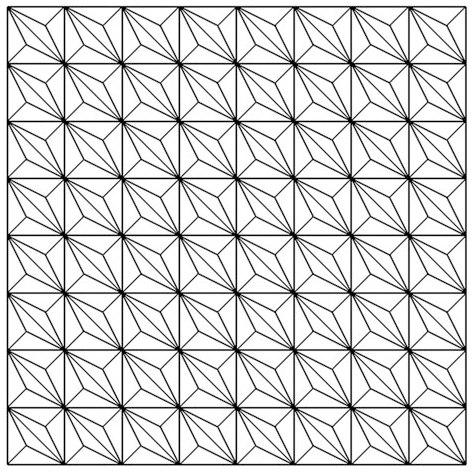
\includegraphics[width=0.78\linewidth]{figures/Chapter_03/Fig_3_09__PDFp125__Bookp113.pdf}
  \captionof{figure}{单位正方形上的单纯形重心加密网格.}\label{fig:barycentric-refinement}
\end{elegantfigure}

在三维重心加密网格上,Scott--Vogelius 空间对 $P_3/P_2^{\mathrm{disc}}$ 曾用于电化学应用,见\textcite{Fuhrmann2009,Fuhrmann2011};也用于湍流模拟,见\textcite{Cuff2015}.
\index{Scott--Vogelius 有限元!三维情形}
\end{note}

\begin{note}[$P_2^{\mathrm{bubble}}/P_1^{\mathrm{disc}}$ 和 $P_3^{\mathrm{bubble}}/P_2^{\mathrm{disc}}$ 空间对]\label{note:bubble-discontinuous-pressure-pairs}
该类空间对由\textcite{CrouzeixRaviart1973} 提出.若要在任意单纯形网格上获得压力为分片线性不连续函数的 inf-sup 稳定空间对,就需要扩充速度空间.事实证明,加入气泡函数,也就是局部函数,便已足够.二维情形下,只需加入所有网格单元的气泡函数;每个三角形单元上的单元气泡函数是三个重心坐标的乘积 $\lambda_1\lambda_2\lambda_3$.

在三维情形下,\textcite{CrouzeixRaviart1973} 提出的扩充由所有单元气泡函数和所有面气泡函数(face bubble functions)组成.对具有重心坐标 $\lambda_1,\ldots,\lambda_4$ 的网格单元 $K$,单元气泡函数为 $\lambda_1\lambda_2\lambda_3\lambda_4$;四个面气泡函数则分别是三个互不相同重心坐标的乘积,例如 $\lambda_1\lambda_2\lambda_3$.因此,每个速度分量有 15 个自由度用于扩充,局部扩充空间的维数为 45.从实际计算角度看,必须考虑到气泡函数是高次多项式,使用它们需要采用高阶求积公式.\textcite[第 553 页]{GreshoSani2000} 认为 $P_2^{\mathrm{bubble}}/P_1^{\mathrm{disc}}$ 空间对是一个很好的选择.

通过气泡函数扩充空间对以获得稳定性的做法可以推广到高阶空间.例如,在\textcite{CrouzeixRaviart1973} 中还给出了二维情形的 $P_3^{\mathrm{bubble}}/P_2^{\mathrm{disc}}$ 空间对.
\index{气泡函数!单元气泡函数}
\index{气泡函数!面气泡函数}
\end{note}

\begin{note}[一阶 Bernardi--Raugel 元 $P_1^{\mathrm{BR}}/P_0^{\mathrm{disc}}$]\label{note:bernardi-raugel-first-order}
构造一阶 Bernardi--Raugel 有限元时,需要在 $P_1(K)$ 空间中加入真正的向量值基函数.设 $\lambda_i$($i=1,\ldots,d+1$)为定义\hyperref[def:appendix-b-31]{B.31} 中的重心坐标.利用这些函数定义面气泡函数(二维时即边气泡函数):
\[
  v_{\mathrm{bub},i}^h
  =\left(\prod_{\substack{j=1\\j\ne i}}^{d+1}\lambda_j\right)n_i,
  \qquad i=1,\ldots,d+1,
\]
其中 $n_i$ 是与顶点 $a_i$ 对面的面 $E_i$ 上的单位外法向量.这些面气泡函数是多项式.局部有限元空间为
\[
  P_1^{\mathrm{BR}}(K)
  =P_1(K)^d\oplus\operatorname{span}\{v_{\mathrm{bub},i}^h:
      i=1,\ldots,d+1\}.
\]
自由度包括顶点处的函数值 $v^h(a_i)$(共 $d(d+1)$ 个数值)以及各面上的通量 $v^h\cdot n_i$(共 $d+1$ 个数值).因此,用于扩充的局部自由度总数为 $(d+1)^2$.

相应的整体速度空间由连续函数构成.两个网格单元 $K_1,K_2$ 在面 $E$ 上相邻时,它们的面气泡函数在 $E$ 上可以组合为连续函数.具体而言,分别使用两个网格单元各自指向外侧的法向量时,面气泡函数在 $E$ 上的迹互为相反数;按此法向量定义的面通量也改变符号,因此 $v_{\mathrm{bub},i}^h|_{K_1}$ 和 $v_{\mathrm{bub},i}^h|_{K_2}$ 前的系数绝对值相同而符号相反.这样,基函数与局部泛函的组合便给出整体连续函数.

整体空间的离散 inf-sup 条件证明基于 Fortin 算子的构造,见\hyperref[lem:fortin-criterion]{引理~\ref{lem:fortin-criterion}}.该算子具有\cref{eq:fortin-operator-construction} 的形式,其中 $P_1^h=P_{\mathrm{Cle}}^h$,另见\cref{note:fortin-detailed-construction}.对每个网格单元 $K$,算子由下列条件定义:
\[
\begin{aligned}
  P_{\mathrm{For}}^h v(a_i)&=P_{\mathrm{Cle}}^h v(a_i),\\
  \int_{E_i}(v-P_{\mathrm{For}}^h v)\cdot n_i\,\mathrm{d}s&=0,
  \qquad i=1,\ldots,d+1.
\end{aligned}
\]
Fortin 判据中的性质\hyperref[eq:fortin-property]{(3.82)} 已由\textcite[引理 II.4]{BernardiRaugel1985} 证明.Bernardi--Raugel 一阶空间对 $P_1^{\mathrm{BR}}/P_0^{\mathrm{disc}}$ 目前只偶尔用于学术研究.
\index{Bernardi--Raugel 有限元!一阶}
\end{note}

\begin{note}[四边形网格单元构成的剖分族]\label{note:bernardi-raugel-quadrilaterals}
\textcite{BernardiRaugel1985} 指出,速度空间的构造及 inf-sup 条件的证明均可推广到由四边形组成的正则剖分族.这一结果曾用于证明四边形网格上不连续压力空间的离散 inf-sup 条件,见笔记\hyperref[note:unmapped-qk-pdisc-2d]{3.143} 和例题\hyperref[ex:unmapped-q2-p1]{3.144}.
\index{Bernardi--Raugel 有限元!四边形网格}
\end{note}

\begin{note}[三维二阶 Bernardi--Raugel 元 $P_2^{\mathrm{BR}}/P_1^{\mathrm{disc}}$]\label{note:bernardi-raugel-second-order-3d}
在四面体网格上,\textcite{BernardiRaugel1985} 提出的局部速度空间为
\[
  P_2^{\mathrm{BR}}(K)
  =P_2(K)^3\oplus\operatorname{span}\{v_{\mathrm{bub},i}^h:
       i=1,\ldots,4\}
       \oplus\bigl(\operatorname{span}\{\lambda_1\lambda_2\lambda_3\lambda_4\}\bigr)^3.
\]
该构造与不连续压力空间配合使用,可视为二维情形下\textcite{CrouzeixRaviart1973} 所引入空间对的推广.$P_2^{\mathrm{BR}}(K)$ 的自由度包括顶点处和边中点处的函数值(来自 $P_2$,共 30 个自由度)、各面上的通量(来自 $\operatorname{span}\{v_{\mathrm{bub},i}^h\}$,共 4 个自由度),以及矩
\[
  \int_K x_i\,\nabla\cdot v^h\,\mathrm{d}x,
  \qquad i=1,2,3.
\]
因此,局部空间的维数为 37.

沿用\cref{note:bernardi-raugel-first-order} 中的相同论证,可知相应的整体速度空间由连续函数组成.通过类似\cref{note:bernardi-raugel-first-order} 所述方式构造 Fortin 算子,可以证明离散 inf-sup 条件\cref{eq:discrete-infsup-condition} 成立.

\textcite{JohnKindlSuciu2010} 给出了 $P_2^{\mathrm{BR}}/P_1^{\mathrm{disc}}$ 空间对的数值模拟.该文选择这一空间对而非 Taylor--Hood 空间对 $P_2/P_1$ 的主要原因,是所用多重网格求解器(见第\hyperref[subsec:multigrid-method]{9.2.2 节})对压力不连续的空间对效率更高.总的来说,据目前所知,这一空间对仍只用于学术研究.
\index{Bernardi--Raugel 有限元!三维二阶}
\end{note}
\subsection{四边形与六面体网格上的不连续压力空间}\label{sec:quadrilateral-discontinuous-pressure}

\begin{note}[$Q_k/P_{k-1}^{\mathrm{disc}}$ 空间对]\label{note:qk-pdisc-mapped-unmapped}
在四边形和六面体网格上,速度协调、压力不连续的常用空间对是 $Q_k/P_{k-1}^{\mathrm{disc}}$,其中 $k\ge2$.例题\hyperref[ex:q1-q0-instability]{3.71} 已说明,$Q_1/P_0^{\mathrm{disc}}=Q_1/Q_0$ 一般不满足离散 inf-sup 稳定性.对于 $k\ge2$,需区分映射型与非映射型 $Q_k/P_{k-1}^{\mathrm{disc}}$ 空间对.

在非映射型空间对中,局部速度空间 $Q_k(K)$ 由参考单元 $\widehat K$ 上的空间经映射定义,而压力空间 $P_{k-1}^{\mathrm{disc}}(K)$ 直接在网格单元 $K$ 上定义.映射型空间对则用参考变换定义速度和压力空间.四边形或六面体参考单元到物理网格单元的映射一般是双线性或三线性映射,因此物理网格单元可能具有曲边.此外,这类变换通常不保持映射函数的类型:多项式经变换后一般不再是多项式.因此,在一般网格上,映射型与非映射型 $Q_k/P_{k-1}^{\mathrm{disc}}$ 空间对并不相同.

本书中所有采用 $Q_k/P_{k-1}^{\mathrm{disc}}$ 空间对的数值模拟,均使用映射型空间.
\index{映射型有限元}
\index{非映射型有限元}
\end{note}

\begin{note}[映射型 $Q_k/P_{k-1}^{\mathrm{disc}}$ 空间对的插值误差]\label{note:mapped-qk-interpolation-error}
对一般网格单元而言,映射后的函数不再是多项式,这会影响 Bramble--Hilbert 引理的应用,见引理\hyperref[lem:appendix-c-5]{C.5}.因此,无法证明最优插值误差估计;\textcite{ArnoldBoffiFalk2002} 给出了这一结论,并展示了相应数值模拟中收敛阶降低的现象.

\textcite{ArnoldBoffiFalk2002} 和\textcite{Matthies2001} 研究了四边形及六面体映射有限元的最优插值误差估计.研究表明,只有对某些特殊网格族,才能得到最优估计.在二维和三维情形下,由初始粗网格经正则一致加密得到的网格族,就属于这类特殊网格族.
\end{note}

\begin{note}[二维非映射型 $Q_k/P_{k-1}^{\mathrm{disc}}$ 空间对]\label{note:unmapped-qk-pdisc-2d}
关于二维非映射型 $Q_k/P_{k-1}^{\mathrm{disc}}$($k\ge2$)有限元空间满足离散 inf-sup 条件\cref{eq:discrete-infsup-condition} 的证明,可见\textcite[第 II 章,定理 3.2]{GiraultRaviart1986}.该证明采用\textcite{BolandNicolaides1983} 的宏单元方法,见定理\hyperref[thm:boland-nicolaides-macroelement-criterion]{3.101}.应用该判据时,需要选取适当的子空间 $\overline V^h\subset V^h$.在\textcite{GiraultRaviart1986} 中,作者选用四边形网格上的一阶 Bernardi--Raugel 空间,见笔记\hyperref[note:bernardi-raugel-quadrilaterals]{3.139}.
\end{note}

\begin{example}[二维非映射型 $Q_2/P_1^{\mathrm{disc}}$ 有限元的离散 inf-sup 条件]\label{ex:unmapped-q2-p1}
采用\textcite{Stenberg1984} 提出的宏单元方法,也可以直接证明二维非映射型 $Q_2/P_1^{\mathrm{disc}}$ 有限元满足离散 inf-sup 条件\cref{eq:discrete-infsup-condition}.只需验证定义\hyperref[def:macroelement-condition]{3.107} 中的宏单元条件.为此,将单个网格单元本身取作宏单元.这样只有一类宏单元,宏单元剖分也就是原网格剖分.

宏单元上的压力是一次函数,即
\[
  Q_M^h=\left\{q^h:\ q^h|_M=a+b_xx+b_yy,\quad
         a,b_x,b_y\in\mathbb{R}\right\}.
\]
$V_{0,M}^h$ 的自由度只有单元内部节点处的自由度.取基函数
$\symbf{\psi}(\bm{x})=(\varphi(\bm{x}),0)^\mathsf{T}$,使其在该节点处取值 $(1,0)^\mathsf{T}$.分部积分给出
\[
  (\nabla\cdot\symbf{\psi},q^h)_M
  =-(\symbf{\psi},\nabla q^h)_M
  =-b_x\int_M\varphi(\bm{x})\,\mathrm{d}x.
\]
由于基函数的积分为正,若 $(\nabla\cdot\symbf{\psi},q^h)_M=0$,便有 $b_x=0$.同理,取基函数 $(0,\varphi(\bm{x}))^\mathsf{T}$ 可得 $b_y=0$.因此
\[
  Q_{\mathrm{grad},M}^h
   =\left\{q^h:\ q^h|_M=a,\quad a\in\mathbb{R}\right\},
\]
于是条件\hyperref[eq:macroelement-condition]{(3.110)} 也成立.
\end{example}

\begin{note}[映射型 $Q_k/P_{k-1}^{\mathrm{disc}}$ 空间对]\label{note:mapped-qk-pdisc}
\textcite{MatthiesTobiska2002} 已证明,任意空间维数 $d$ 下,映射型 $Q_k/P_{k-1}^{\mathrm{disc}}$ 空间对均满足离散 inf-sup 条件\cref{eq:discrete-infsup-condition}.证明采用\textcite{BolandNicolaides1983} 的宏单元方法,见定理\hyperref[thm:boland-nicolaides-macroelement-criterion]{3.101}.为构造该定理假设所需的子空间,作者把笔记\hyperref[note:bernardi-raugel-quadrilaterals]{3.139} 中提到的二维情形——将三角形上的 Bernardi--Raugel 元推广至四边形——的证明,进一步推广到任意维数的四边形类型网格单元.
\end{note}

\subsection{最低阶非协调有限元空间}\label{sec:lowest-order-nonconforming}

\begin{note}[非协调有限元空间]\label{note:nonconforming-finite-elements}
从最一般的意义上说,只要有限元空间不是变分问题所用函数空间的子空间,相应的有限元方法就是非协调的(non-conforming).例如,若区域 $\Omega$ 的边界包含曲线部分,而用边界为多边形或多面体的区域 $\Omega^h$ 近似它,也可能出现这种情形.不过,通常只有当空间不包含关系源自有限元空间的构造,且与具体问题无关时,才称该有限元方法为非协调有限元方法.

对不可压缩流模型而言,考虑非协调离散化,可以构造满足离散 inf-sup 条件\cref{eq:discrete-infsup-condition} 的最低阶有限元空间对.非协调性只出现在速度空间,而不出现在压力空间,即 $V^h\not\subset V$,但 $Q^h\subset Q$.

这里重点讨论最低阶非协调离散化,因为它们是不可压缩流问题中最重要的非协调方法.在单纯形网格上,这种离散化称为 Crouzeix--Raviart 有限元 $P_1^{\mathrm{nc}}/P_0$.速度用分片线性函数逼近,该函数在网格单元各面的重心处连续;详细定义见例题\hyperref[ex:appendix-b-43]{B.43}.压力则用分片常数函数逼近,见例题\hyperref[ex:appendix-b-37]{B.37}.

将这一方法推广到四边形和六面体网格,可得到 Rannacher--Turek 元 $Q_1^{\mathrm{rot}}/Q_0$.其中速度由旋转的 $d$-线性函数逼近,这些函数在网格单元各面上的自由度连续,见例题\hyperref[ex:appendix-b-53]{B.53};压力用分片常数函数离散,见例题\hyperref[ex:appendix-b-49]{B.49}.

最低阶非协调有限元除了阶数低之外,还有其他优点.它们可用于构造高阶不可压缩流离散化的高效多重网格求解器或预条件子,见第\hyperref[subsec:multigrid-method]{9.2.2 节}.在并行计算机上实现 Navier--Stokes 方程求解程序时,非协调离散化通常比协调有限元方法所需的通信开销更少.不过,从数值分析角度看,非协调有限元往往更复杂.

离散 inf-sup 条件的证明依赖于构造算子 $V\to V^h$,使得对每个函数 $v\in V$,该算子满足与 Fortin 算子条件\hyperref[eq:fortin-property]{(3.82)} 相应的性质.
\index{非协调有限元}
\index{Crouzeix--Raviart 有限元}
\index{Rannacher--Turek 元}
\end{note}

\begin{note}[非协调 $Q_1^{\mathrm{rot}}/Q_0$ 有限元空间对]\label{note:nonconforming-qrot-pairs}
这类有限元空间对由\textcite{RannacherTurek1992} 引入并分析,之后\textcite{Schieweck1997} 对其作了全面研究.它们定义在四边形或六面体网格单元上.其局部速度空间称为旋转双线性有限元空间,定义如下:
\[
  Q_1^{\mathrm{rot}}(\widehat K)=
  \begin{cases}
    \operatorname{span}\{1,\widehat x_1,\widehat x_2,
                  \widehat x_1^2-\widehat x_2^2\},&d=2,\\
    \operatorname{span}\{1,\widehat x_1,\widehat x_2,\widehat x_3,
       \widehat x_1^2-\widehat x_2^2,\widehat x_2^2-\widehat x_3^2\},&d=3,
  \end{cases}
\]
\[
  Q_1^{\mathrm{rot}}(K)=
  \left\{p=\widehat p\circ F_K^{-1}:
                 \widehat p\in Q_1^{\mathrm{rot}}(\widehat K)\right\},
  \qquad \widehat K=[-1,1]^d.
\]
根据所采用的局部泛函不同,$Q_1^{\mathrm{rot}}$ 有两种类型.令 $\mathcal{E}(K)$ 表示 $K$ 的所有 $(d-1)$ 维面,并设 $K'$ 是 $K$ 的一个邻接单元.以面均值为自由度的有限元空间定义为
\begin{equation}\label{eq:qrot-mean-value-space}
  \begin{aligned}
  Q_{1,\mathrm{mean}}^{\mathrm{rot}}
   =\{v\in L^2(\Omega):\
  &\left.v\right|_K\in Q_1^{\mathrm{rot}}(K)
       \quad\forall K\in\mathcal{T}^h,\\
  &\int_E\left(\left.v\right|_K-\left.v\right|_{K'}\right)\,\mathrm{d}s=0
  \}.
  \end{aligned}
\end{equation}
第二个条件要求每一对相邻网格单元在其公共面 $E\in\mathcal{E}(K)\cap\mathcal{E}(K')$ 上的函数积分相等.
以面重心处的点值为自由度的有限元空间则为
\[
  \begin{aligned}
  Q_{1,\mathrm{point}}^{\mathrm{rot}}
  =\{v\in L^2(\Omega):\
    \left.v\right|_K\in Q_1^{\mathrm{rot}}(K)
      \ \forall K\in\mathcal{T}^h,\\[-2pt]
  v\text{ 在每个网格单元的面重心处连续}\}.
  \end{aligned}
\]
一般而言,以面均值为自由度和以面重心点值为自由度的 $Q_1^{\mathrm{rot}}$ 空间并不等价.压力用分片常数函数逼近.
\end{note}

\begin{note}[双线性型 $b(\cdot,\cdot)$ 的延拓]\label{note:nonconforming-bilinear-form}
对于非协调空间 $V^h\not\subset V$,\hyperref[eq:incompressible-bilinear-form]{式(3.34)} 中的双线性型 $b(\cdot,\cdot)$ 并未对所有 $v^h\in V^h$ 定义,因此需要适当地扩展其定义域.由于非协调有限元函数也是分片多项式,一种自然做法是在每个网格单元上分别计算双线性型,再对所有网格单元求和.因此,非协调有限元近似应采用\hyperref[eq:discrete-bilinear-form-b]{式(3.53)} 给出的双线性型 $b^h(\cdot,\cdot)$.
\end{note}

\begin{note}[施加 Dirichlet 边界条件]\label{note:nonconforming-dirichlet}
对以面重心点值为自由度的非协调有限元空间,在边界面重心处取 Dirichlet 边界条件的值.对以面均值为自由度的空间,则计算边界条件在相应边界面上的积分,再除以该面的面积,以确定边界自由度.若施加齐次 Dirichlet 边界条件,两种方法所得边界自由度均为零.
\end{note}

\Needspace{8\baselineskip}
\begin{lemma}[$P_1^{\mathrm{nc}}$ 与 $Q_1^{\mathrm{rot}}$ 中的范数]\label{lem:nonconforming-energy-norm}
考虑齐次 Dirichlet 边界条件.定义
\[
  a_h(v^h,w^h)
  :=\sum_{K\in\mathcal{T}^h}
       (\nabla v^h,\nabla w^h)_K.
\]
则映射 $v^h\mapsto a_h(v^h,v^h)^{1/2}$ 分别在 $P_1^{\mathrm{nc}}$ 和 $Q_1^{\mathrm{rot}}$ 上定义一个范数.
\end{lemma}

\begin{proof}
只需验证定义\hyperref[def:appendix-a-6]{A.6} 中范数的各项性质.

\textit{i)} 若 $v^h=0$ 于 $\Omega$,则显然
\[
  a_h(v^h,v^h)^{1/2}
  =\left(\sum_{K\in\mathcal{T}^h}
      (\nabla v^h,\nabla v^h)_K\right)^{1/2}=0.
\]
反之,若 $a_h(v^h,v^h)^{1/2}=0$,则 $v^h$ 在每个网格单元上都是常数,因为其在各单元上的梯度均为零.只要知道 $v^h$ 在该单元内一点处的值,就能确定这个常数.

$P_1^{\mathrm{nc}}$ 和采用面重心点值自由度的 $Q_1^{\mathrm{rot}}$ 有限元函数,其自由度都是各面重心处的函数值.在边界面上,这些值由边界条件给定,因而为零.因此,与边界相邻的网格单元上,常数值为零.由此,这些单元其他面重心处的函数值也为零.由于有限元函数在面重心处连续,相邻单元上的常数值也为零.逐个向相邻单元推进,可知所有网格单元上的常数均为零,即 $v^h=0$ 于 $\Omega$.

对以面均值为自由度的 $Q_1^{\mathrm{rot}}$,齐次 Dirichlet 边界条件要求边界面上的积分为零.只有零常数满足该条件,因此所有与边界面相邻的网格单元上函数均为零.于是,这些单元其他各面上的积分也为零.根据面均值空间的定义\cref{eq:qrot-mean-value-space},相邻网格单元上的面积分也必须为零.由于 $v^h$ 在这些单元上同样为常数,其常数值也只能为零.再次逐个向相邻单元推进,即得 $v^h=0$ 于 $\Omega$.

\textit{ii)} 对任意 $\alpha\in\mathbb{R}$,直接计算得到
\[
\begin{aligned}
  a_h(\alpha v^h,\alpha v^h)^{1/2}
   &=\left(\sum_{K\in\mathcal{T}^h}
      (\nabla(\alpha v^h),\nabla(\alpha v^h))_K\right)^{1/2}\\
   &=|\alpha|
      \left(\sum_{K\in\mathcal{T}^h}
      (\nabla v^h,\nabla v^h)_K\right)^{1/2}
    =|\alpha|\,a_h(v^h,v^h)^{1/2}.
\end{aligned}
\]

\textit{iii)} 三角不等式由各网格单元上的三角不等式和求和形式的 Cauchy--Schwarz 不等式\hyperref[eq:appendix-a-2]{A.2} 推出:
\[
\begin{aligned}
  a_h(v^h+w^h,v^h+w^h)
   &=\sum_{K\in\mathcal{T}^h}
       \|\nabla(v^h+w^h)\|_{L^2(K)}^2\\
   &\le\sum_{K\in\mathcal{T}^h}
       \bigl(\|\nabla v^h\|_{L^2(K)}
             +\|\nabla w^h\|_{L^2(K)}\bigr)^2\\
   &\le
    \left(
      \left[\sum_{K\in\mathcal{T}^h}
        \|\nabla v^h\|_{L^2(K)}^2\right]^{1/2}
      \right.\\[-2pt]
   &\hspace{2em}\left.
      +\left[\sum_{K\in\mathcal{T}^h}
        \|\nabla w^h\|_{L^2(K)}^2\right]^{1/2}
    \right)^2\\
   &=\bigl(a_h(v^h,v^h)^{1/2}
           +a_h(w^h,w^h)^{1/2}\bigr)^2.
\end{aligned}
\]
两边开平方,便得到所需三角不等式.
\end{proof}

\begin{theorem}[最低阶 Crouzeix--Raviart 有限元 $P_1^{\mathrm{nc}}/P_0$ 的 inf-sup 条件]\label{thm:crouzeix-raviart-infsup}
最低阶 Crouzeix--Raviart 有限元空间对 $P_1^{\mathrm{nc}}/P_0$ 满足离散 inf-sup 条件\cref{eq:discrete-infsup-condition},或等价地满足\cref{eq:discrete-infsup-condition-equivalent}.条件\cref{eq:discrete-infsup-condition} 中的常数 $\beta_{\mathrm{is}}^h$ 可取为连续 inf-sup 条件\cref{eq:infsup-condition} 中的常数 $\beta_{\mathrm{is}}$.
\end{theorem}

\begin{proof}
证明用到 $P_1^{\mathrm{nc}}$ 中函数是分片线性的、$P_0$ 中函数是分片常数这两个性质.

第一步,对任意 $v\in V$,构造到 $V^h=P_1^{\mathrm{nc}}$ 的适当插值 $\mathcal{P}_E^h v$.$P_1^{\mathrm{nc}}$ 中的函数由其在网格单元各面重心处的值确定.记 $\mathcal{E}$ 为所有网格面的集合,$m_E$ 为面 $E$ 的重心,$\mathcal{E}^h$ 为所有内部面的集合.定义 $\mathcal{P}_E^h v$ 在各面重心处的值为
\begin{equation}\label{eq:crouzeix-raviart-interpolant}
  \mathcal{P}_E^h v(m_E)=
  \begin{cases}
    \displaystyle\frac{1}{|E|}\int_E v(s)\,\mathrm{d}s,
       & E\in\mathcal{E}^h,\\[6pt]
    0, & E\in\mathcal{E}\setminus\mathcal{E}^h.
  \end{cases}
\end{equation}
这个构造正是利用有限元空间定义中的整体泛函作插值,见 $P_1^{\mathrm{nc}}$ 空间的定义\hyperref[ex:appendix-b-43]{B.43}.这些泛函都是连续的.

第二步,证明对任意 $q^h\in Q^h$,$b^h(\mathcal{P}_E^h v,q^h)$ 与 $b(v,q^h)$ 之间的关系.由于 $q^h$ 分片常数,分部积分可得
\[
\begin{aligned}
  b^h(\mathcal{P}_E^h v,q^h)
   &=-\sum_{K\in\mathcal{T}^h}
       \int_K(\nabla\cdot\mathcal{P}_E^h v)\,q^h(\bm{x})\,\mathrm{d}x\\
   &=-\sum_{K\in\mathcal{T}^h}
       \left.q^h\right|_K
       \int_K\nabla\cdot\mathcal{P}_E^h v(\bm{x})\,\mathrm{d}x\\
   &=-\sum_{K\in\mathcal{T}^h}
       \left.q^h\right|_K
       \sum_{E\subset\partial K}
       \int_E\mathcal{P}_E^h v\cdot n_E(s)\,\mathrm{d}s.
\end{aligned}
\]
由于 $\mathcal{P}_E^h v\cdot n_E|_E$ 是线性函数,用中点求积公式即可精确计算其积分.因此
\[
\begin{aligned}
  b^h(\mathcal{P}_E^h v,q^h)
   &=-\sum_{K\in\mathcal{T}^h}
       \left.q^h\right|_K
       \sum_{E\subset\partial K}
       |E|\,\mathcal{P}_E^h v(m_E)\cdot n_E\\
   &=-\sum_{K\in\mathcal{T}^h}
       \left.q^h\right|_K
       \sum_{E\subset\partial K}
       \int_E v\cdot n_E(s)\,\mathrm{d}s\\
   &=-\sum_{K\in\mathcal{T}^h}
       \left.q^h\right|_K
       \int_K\nabla\cdot v(\bm{x})\,\mathrm{d}x\\
   &=-\sum_{K\in\mathcal{T}^h}
       \int_K(\nabla\cdot v)q^h(\bm{x})\,\mathrm{d}x\\
   &=b^h(v,q^h)=b(v,q^h).
\end{aligned}
\]
其中第二步用了 $\mathcal{P}_E^h v(m_E)$ 的定义,随后再次分部积分.综上,
\begin{equation}\label{eq:crouzeix-raviart-fortin-identity}
  b^h(\mathcal{P}_E^h v,q^h)=b(v,q^h)
  \qquad\forall v\in V,\ \forall q^h\in Q^h.
\end{equation}
该式对应于 Fortin 算子条件\hyperref[eq:fortin-property]{(3.82)} 的第一项性质.

接下来证明 $\|\mathcal{P}_E^h v\|_{V^h}\le\|v\|_V$.任取网格单元 $K\in\mathcal{T}^h$.由于 $\Delta\mathcal{P}_E^h v|_K=0$,且 $\nabla\mathcal{P}_E^h v\cdot n_E|_E$ 在面 $E$ 上为常数,分部积分给出
\[
\begin{aligned}
  \|\nabla\mathcal{P}_E^h v\|_{L^2(K)}^2
   &=\int_K\nabla\mathcal{P}_E^h v:
             \nabla\mathcal{P}_E^h v\,\mathrm{d}x\\
   &=\sum_{E\subset\partial K}
       \int_E\mathcal{P}_E^h v\cdot
          (\nabla\mathcal{P}_E^h v)n_E\,\mathrm{d}s
       -\int_K\mathcal{P}_E^h v\cdot
          \Delta\mathcal{P}_E^h v\,\mathrm{d}x\\
   &=\sum_{E\subset\partial K}
       \left.(\nabla\mathcal{P}_E^h v)n_E\right|_E
          \cdot\int_E\mathcal{P}_E^h v(s)\,\mathrm{d}s.
\end{aligned}
\]
被积函数是线性的,故中点求积公式可精确计算其积分.再利用定义\cref{eq:crouzeix-raviart-interpolant}、分部积分、$\Delta\mathcal{P}_E^h v|_K=0$ 以及 Cauchy--Schwarz 不等式\hyperref[eq:appendix-a-10]{A.10},得到
\[
\begin{aligned}
  \|\nabla\mathcal{P}_E^h v\|_{L^2(K)}^2
   &=\sum_{E\subset\partial K}
       \left.(\nabla\mathcal{P}_E^h v)n_E\right|_E
       \cdot |E|\,\mathcal{P}_E^h v(m_E)\\
   &=\sum_{E\subset\partial K}
       \left.(\nabla\mathcal{P}_E^h v)n_E\right|_E
       \cdot\int_E v(s)\,\mathrm{d}s\\
   &=\sum_{E\subset\partial K}
       \int_E v\cdot(\nabla\mathcal{P}_E^h v)n_E(s)\,\mathrm{d}s\\
   &=\int_K\nabla\mathcal{P}_E^h v:\nabla v\,\mathrm{d}x
       +\int_K v\cdot\Delta\mathcal{P}_E^h v\,\mathrm{d}x\\
   &\le \|\nabla\mathcal{P}_E^h v\|_{L^2(K)}
         \|\nabla v\|_{L^2(K)}.
\end{aligned}
\]
结合此估计和求和形式的 Cauchy--Schwarz 不等式\hyperref[eq:appendix-a-2]{A.2},有
\[
\begin{aligned}
  \|\mathcal{P}_E^h v\|_{V^h}^2
   &=\sum_{K\in\mathcal{T}^h}
       \|\nabla\mathcal{P}_E^h v\|_{L^2(K)}^2\\
   &\le\sum_{K\in\mathcal{T}^h}
       \|\nabla\mathcal{P}_E^h v\|_{L^2(K)}
       \|\nabla v\|_{L^2(K)}\\
   &\le\|\mathcal{P}_E^h v\|_{V^h}\,\|v\|_V.
\end{aligned}
\]
若 $\|\mathcal{P}_E^h v\|_{V^h}\ne0$,约去该因子;若其为零,结论显然.于是
\begin{equation}\label{eq:crouzeix-raviart-fortin-bound}
  \|\mathcal{P}_E^h v\|_{V^h}\le\|v\|_V
  \qquad\forall v\in V.
\end{equation}
该估计对应 Fortin 算子条件\hyperref[eq:fortin-property]{(3.82)} 的第二项性质.

由\cref{eq:crouzeix-raviart-fortin-identity,eq:crouzeix-raviart-fortin-bound},得到
\[
  \sup_{v\in V,\ v\ne0}
      \frac{b(v,q^h)}{\|v\|_V}
  \le
  \sup_{v\in V,\ v\ne0}
      \frac{b^h(\mathcal{P}_E^h v,q^h)}
           {\|\mathcal{P}_E^h v\|_{V^h}}
  \le
  \sup_{v^h\in V^h,\ v^h\ne0}
      \frac{b^h(v^h,q^h)}{\|v^h\|_{V^h}}.
\]
最后一步是因为所有 $\mathcal{P}_E^h v$ 均属于 $V^h$,其上确界不超过在整个 $V^h$ 上取的上确界.又由于 $Q^h\subset Q$,连续 inf-sup 条件\cref{eq:infsup-condition} 给出
\[
  \beta_{\mathrm{is}}\|q^h\|_Q
  \le
  \sup_{v\in V,\ v\ne0}\frac{b(v,q^h)}{\|v\|_V}
  \le
  \sup_{v^h\in V^h,\ v^h\ne0}
        \frac{b^h(v^h,q^h)}{\|v^h\|_{V^h}}
  \qquad\forall q^h\in Q^h.
\]
这正是离散 inf-sup 条件\cref{eq:discrete-infsup-condition-equivalent},其中 $\beta_{\mathrm{is}}^h=\beta_{\mathrm{is}}$.证毕.
\end{proof}

\begin{note}[各向异性网格单元]\label{note:crouzeix-raviart-anisotropic}
注意,定理\hyperref[thm:crouzeix-raviart-infsup]{3.151} 的证明没有对单纯形网格单元的长宽比作任何特殊要求.此外,离散 inf-sup 常数等于连续 inf-sup 常数,因此不依赖于网格.由此,即使网格单元高度各向异性,也就是 $h_K/\rho_K$ 很大,离散 inf-sup 条件仍一致成立,有限元问题仍是适定的.
\end{note}

\begin{note}[$Q_1^{\mathrm{rot}}/Q_0$ 空间对的离散 inf-sup 条件]\label{note:qrot-infsup}
\textcite{RannacherTurek1992} 通过构造 Fortin 算子证明了 $Q_1^{\mathrm{rot}}/Q_0$ 空间对满足离散 inf-sup 条件\cref{eq:discrete-infsup-condition},参见引理\hyperref[lem:fortin-criterion]{3.78}.他们使用了整体插值算子;该算子由 $Q_1^{\mathrm{rot}}(K)$ 上的典范局部插值算子构造.对以面均值为自由度的版本,Fortin 算子满足性质\hyperref[eq:fortin-property]{(3.82)} 的证明与定理\hyperref[thm:crouzeix-raviart-infsup]{3.151} 的证明类似.

\textcite{Schieweck1997} 对 $Q_1^{\mathrm{rot}}$ 有限元空间的若干实现作了全面分析.与\textcite{RannacherTurek1992} 的分析相比,该分析放宽了证明 inf-sup 条件时对网格的假设.
\end{note}

\begin{note}[非映射型 $Q_1^{\mathrm{rot}}/Q_0$ 有限元空间]\label{note:unmapped-qrot}
这类有限元空间也有非映射型(非参数型)版本,即直接在网格单元 $K$ 上定义多项式.\textcite{RannacherTurek1992} 证明,与映射型(参数型)$Q_1^{\mathrm{rot}}/Q_0$ 有限元相比,这些版本在更一般的网格上仍满足 inf-sup 稳定性,例如强烈非均匀的网格.$Q_1^{\mathrm{rot}}/Q_0$ 有限元共有四种类型;在扰动网格上,只有以面均值为自由度的非映射型 $Q_1^{\mathrm{rot}}/Q_0$ 有限元达到最优收敛阶.
\end{note}

\begin{note}[$Q_1^{\mathrm{rot}}/Q_0$ 有限元空间的实际使用]\label{note:qrot-practical-use}
本书的数值模拟在二维中采用以面均值为自由度的映射型 $Q_1^{\mathrm{rot}}$ 有限元空间,在三维中采用以面重心点值为自由度的映射型 $Q_1^{\mathrm{rot}}$ 有限元空间.当 $d=3$ 时,映射型面均值空间所要求的网格单元面上积分相等关系,包含依赖于具体网格单元 $K$ 的权函数.对所有网格单元计算这些权函数会带来额外开销,因此\textcite[第 21 页]{Schieweck1997} 建议在三维中采用更简单的映射型面重心点值版本.
\end{note}

\begin{note}[高阶非协调有限元空间]\label{note:higher-order-nonconforming}
\textcite{MatthiesTobiska2005} 将二维 $P_1^{\mathrm{nc}}/P_0$ 空间对推广到任意阶非协调有限元空间,并证明所提出的空间对满足离散 inf-sup 条件\cref{eq:discrete-infsup-condition}.
\index{非协调有限元!高阶}
\end{note}

\subsection{计算离散 inf-sup 常数}\label{sec:computing-discrete-infsup}

\begin{note}[离散 inf-sup 条件中的常数]\label{note:discrete-infsup-independence}
离散 inf-sup 条件\cref{eq:discrete-infsup-condition} 中常数 $\beta_{\mathrm{is}}^h$ 的实际大小值得关注,因为它会进入有限元误差估计等结果.当然,该常数取决于具体空间,尤其取决于区域和所用网格.
\end{note}

\begin{note}[上确界的取值]\label{note:discrete-infsup-supremum}
固定 $q^h\in Q^h$.由式\hyperref[eq:discrete-bilinear-form-b]{(3.53)} 定义的 $b^h(\,\cdot\,,q^h)$ 是 $V^h$ 上的线性泛函.其线性来自积分的线性;利用三角不等式、Cauchy--Schwarz 不等式\hyperref[eq:appendix-a-10]{A.10}、求和形式的 Cauchy--Schwarz 不等式\hyperref[eq:appendix-a-2]{A.2},以及当 $\Omega=K$ 时的估计\cref{eq:divergence-gradient-bound-h1},可知该泛函有界:
\[
\begin{aligned}
  |b^h(v^h,q^h)|
   &\le \sum_{K\in\mathcal{T}^h}
        \left|(\nabla\cdot v^h,q^h)_K\right|\\
   &\le \sum_{K\in\mathcal{T}^h}
        \|\nabla\cdot v^h\|_{L^2(K)}
        \|q^h\|_{L^2(K)}\\
   &\le
       \left(\sum_{K\in\mathcal{T}^h}
         \|\nabla\cdot v^h\|_{L^2(K)}^2\right)^{1/2}
       \left(\sum_{K\in\mathcal{T}^h}
         \|q^h\|_{L^2(K)}^2\right)^{1/2}\\
   &\le C
       \left(\sum_{K\in\mathcal{T}^h}
         \|\nabla v^h\|_{L^2(K)}^2\right)^{1/2}
       \|q^h\|_{L^2(\Omega)}\\
   &=C\|v^h\|_{V^h}\,\|q^h\|_{L^2(\Omega)}.
\end{aligned}
\]
根据 Riesz 表示定理\hyperref[thm:appendix-b-3]{B.3},存在 $v_b^h\in V^h$,使得
\begin{equation}\label{eq:discrete-riesz-representation}
  (v_b^h,v^h)_{V^h}=b^h(v^h,q^h)
  \qquad\forall v^h\in V^h.
\end{equation}
于是
\[
  b^h(v^h,q^h)
   =(v_b^h,v^h)_{V^h}
   \le \|v_b^h\|_{V^h}\,\|v^h\|_{V^h}
   \qquad\forall v^h\in V^h,
\]
从而得到上确界的上界
\begin{equation}\label{eq:discrete-infsup-sup-upper-bound}
  \sup_{v^h\in V^h\setminus\{0\}}
      \frac{b^h(v^h,q^h)}{\|v^h\|_{V^h}}
  \le \|v_b^h\|_{V^h}.
\end{equation}
而且这个上界可以取到.特别地,令 $v^h=v_b^h$,由\cref{eq:discrete-riesz-representation} 可得
\begin{equation}\label{eq:discrete-infsup-sup-attained}
  \frac{b^h(v_b^h,q^h)}{\|v_b^h\|_{V^h}}
  =\frac{\|v_b^h\|_{V^h}^2}{\|v_b^h\|_{V^h}}
  =\|v_b^h\|_{V^h}.
\end{equation}
结合\cref{eq:discrete-infsup-sup-upper-bound,eq:discrete-infsup-sup-attained},可知
\[
  v_b^h
   =\operatorname*{arg\,sup}_{v^h\in V^h\setminus\{0\}}
       \frac{b^h(v^h,q^h)}{\|v^h\|_{V^h}}.
\]

由此可得,离散 inf-sup 常数为
\begin{equation}\label{eq:discrete-infsup-constant-riesz}
  \left(\beta_{\mathrm{is}}^h\right)^2
   =\inf_{q^h\in Q^h\setminus\{0\}}
      \sup_{v^h\in V^h\setminus\{0\}}
      \frac{\bigl[b^h(v^h,q^h)\bigr]^2}
           {\|v^h\|_{V^h}^2\,\|q^h\|_{Q^h}^2}
   =\inf_{q^h\in Q^h\setminus\{0\}}
      \frac{\|v_b^h\|_{V^h}^2}{\|q^h\|_{Q^h}^2}.
\end{equation}
到这里为止,对连续 inf-sup 条件也可以作类似论证.
\end{note}

\begin{note}[计算离散 inf-sup 常数的广义特征值问题]\label{note:discrete-infsup-generalized-eigenproblem}
设 $\{\psi_i^h\}_{i=1}^{N_u}$ 和 $\{\xi_i^h\}_{i=1}^{N_p}$ 分别是 $V^h$ 和 $Q^h$ 的一组基.定义 Gram 矩阵(或质量矩阵)
\[
  M_V=\bigl[(\psi_j^h,\psi_i^h)_{V^h}\bigr]_{i,j=1}^{N_u},
  \qquad
  M_Q=\bigl[(\xi_j^h,\xi_i^h)_{Q^h}\bigr]_{i,j=1}^{N_p},
\]
以及矩阵
\[
  B=\bigl[b^h(\psi_j^h,\xi_i^h)\bigr],
  \qquad i=1,\ldots,N_p,\quad j=1,\ldots,N_u.
\]
相应地,有限元函数可表示为
\[
  v^h=\sum_{i=1}^{N_u}v_i\psi_i^h,\qquad
  v_b^h=\sum_{i=1}^{N_u}b_i\psi_i^h,\qquad
  q^h=\sum_{i=1}^{N_p}q_i\xi_i^h,
\]
其中系数向量分别记为 $\bm{v}$、$\bm{b}$ 和 $\bm{q}$.这样,$V^h$ 与 $Q^h$ 中的内积以及双线性型 $b^h(\cdot,\cdot)$ 都可用矩阵和向量表示,例如
\[
\begin{aligned}
  (v_b^h,v^h)_{V^h}
    &=\bm{b}^T M_V\bm{v},\\
  b^h(v^h,q^h)
    &=\bm{v}^T B^T\bm{q},\\
  \|v_b^h\|_{V^h}^2
    &=\bm{b}^T M_V\bm{b}.
\end{aligned}
\]
因此,\cref{eq:discrete-riesz-representation} 可写为
\[
  \bm{b}^T M_V\bm{v}
    =\bm{v}^T B^T\bm{q}
  \quad\Longleftrightarrow\quad
  \bm{v}^T M_V\bm{b}
    =\bm{v}^T B^T\bm{q}
  \qquad\forall\bm{v}\in\mathbb{R}^{N_u},
\]
因而
\[
  M_V\bm{b}=B^T\bm{q}
  \quad\Longrightarrow\quad
  \bm{b}=M_V^{-1}B^T\bm{q}.
\]
将此表达式代入\cref{eq:discrete-infsup-constant-riesz},可得
\[
\begin{aligned}
  \left(\beta_{\mathrm{is}}^h\right)^2
   &=\inf_{\bm{q}\in\mathbb{R}^{N_p}\setminus\{0\}}
       \frac{\bm{b}^T M_V\bm{b}}
            {\bm{q}^T M_Q\bm{q}}\\
   &=\inf_{\bm{q}\in\mathbb{R}^{N_p}\setminus\{0\}}
       \frac{\bm{q}^T B M_V^{-T}M_V M_V^{-1}B^T\bm{q}}
            {\bm{q}^T M_Q^T\bm{q}}\\
   &=\inf_{\bm{q}\in\mathbb{R}^{N_p}\setminus\{0\}}
       \frac{\bm{q}^T B M_V^{-1}B^T\bm{q}}
            {\bm{q}^T M_Q\bm{q}},
\end{aligned}
\]
这里用了 $M_V$ 和 $M_Q$ 对称且正定这一事实.令 $\bm{y}=M_Q^{1/2}\bm{q}$,上式可改写为 Rayleigh 商:
\[
  \frac{
    \bm{y}^T
       \bigl(M_Q^{-1/2}B M_V^{-1}B^T M_Q^{-1/2}\bigr)\bm{y}}
       {\bm{y}^T\bm{y}}.
\]
根据 Rayleigh 商的性质,见引理\hyperref[lem:appendix-a-19]{A.19},其下确界可以取到,且等于下列特征值问题的最小特征值:
\[
  M_Q^{-1/2}B M_V^{-1}B^T M_Q^{-1/2}\bm{y}
   =\lambda\bm{y},
  \qquad \bm{y}=M_Q^{1/2}\bm{q}.
\]
两边左乘 $M_Q^{1/2}$,可知这等价于求解广义特征值问题
\begin{equation}\label{eq:generalized-eigenvalue}
  B M_V^{-1}B^T\bm{q}
   =\lambda M_Q\bm{q}.
\end{equation}
最小特征值的平方根就是离散 inf-sup 常数 $\beta_{\mathrm{is}}^h$.
\index{离散 inf-sup 常数}
\index{广义特征值问题}
\end{note}

\begin{note}[实际计算中的一个问题]\label{note:discrete-infsup-practical}
通常,离散压力空间取 $L^2(\Omega)$ 的子空间,而不取 $L_0^2(\Omega)$ 的子空间,见笔记\hyperref[note:pressure-space-l2]{4.70};压力的加法常数则通过其他方式固定.采用这种处理时,矩阵 $B$ 的核由常数向量张成,且矩阵亏秩为一,见引理\hyperref[lem:constant-pressure-kernel]{4.71}.因此,广义特征值问题\cref{eq:generalized-eigenvalue} 的最小特征值为零;此时,第二小特征值的平方根才是离散 inf-sup 常数 $\beta_{\mathrm{is}}^h$.
\end{note}

\section{Helmholtz 分解}\label{sec:helmholtz-decomposition}

\begin{note}[本节内容]\label{note:helmholtz-contents}
本节介绍 $L^2(\Omega)$ 中向量场的一种分解,这种分解对不可压缩流问题十分重要.利用该分解,可以精确描述某些体力对速度和压力的影响,参见笔记\hyperref[note:force-on-velocity-pressure]{4.12}.
\end{note}

\begin{definition}[旋度与 curl]\label{def:rotation-curl}
有些算子被称为旋度(rotation)或 curl 算子,其定义取决于向量场所在的空间维数.

设 $v(\bm{x})=(v_1(\bm{x}),v_2(\bm{x}),v_3(\bm{x}))^\mathsf{T}$、$\bm{x}=(x,y,z)^\mathsf{T}$ 是区域 $\Omega\subset\mathbb{R}^3$ 上足够光滑的向量场,则 $v(\bm{x})$ 的旋度或 curl 定义为
\begin{equation}\label{eq:curl-vector-3d}
  \setlength{\arraycolsep}{3pt}%
  \nabla\times v(\bm{x})
  =\det\begin{pmatrix}
       \bm{i}&\bm{j}&\bm{k}\\
       \partial_x&\partial_y&\partial_z\\
       v_1(\bm{x})&v_2(\bm{x})&v_3(\bm{x})
      \end{pmatrix}
  =\begin{pmatrix}
       \partial_yv_3-\partial_zv_2\\
       \partial_zv_1-\partial_xv_3\\
       \partial_xv_2-\partial_yv_1
    \end{pmatrix}(\bm{x}).
\end{equation}

设 $v(\bm{x})=(v_1(\bm{x}),v_2(\bm{x}))^\mathsf{T}$、$\bm{x}=(x,y)^\mathsf{T}$ 是二维区域 $\Omega$ 上的向量场.形式上可将其扩充为三维向量场 $v(\bm{x})=(v_1(\bm{x}),v_2(\bm{x}),0)^\mathsf{T}$.此时,\cref{eq:curl-vector-3d} 的前两个分量为零,右端的第三个分量记作
\begin{equation}\label{eq:curl-vector-2d}
  \operatorname{curl}v(\bm{x})
    =\bigl(\partial_xv_2-\partial_yv_1\bigr)(\bm{x}).
\end{equation}

对二维区域上的标量场 $v(\bm{x})$,其中 $\bm{x}=(x,y)^\mathsf{T}$,其 curl 定义为向量场
\begin{equation}\label{eq:curl-scalar-2d}
  \operatorname{curl}v(\bm{x})
    =\begin{pmatrix}-\partial_yv\\[2pt]\partial_xv\end{pmatrix}(\bm{x}).
\end{equation}
\index{旋度算子}
\index{旋度}
\end{definition}

\begin{note}[旋度或 curl 算子的性质]\label{note:curl-identities}
直接计算可知,在二维情形下,对足够光滑的函数有
\begin{equation}\label{eq:curl-curl-2d}
  \operatorname{curl}(\operatorname{curl}v)(\bm{x})
     =-\Delta v(\bm{x}).
\end{equation}
在三维情形下,
\begin{equation}\label{eq:curl-curl-3d}
  \nabla\times(\nabla\times v)(\bm{x})
     =-\Delta v(\bm{x})
       +\nabla(\nabla\cdot v)(\bm{x}).
\end{equation}
将二维向量场形式上扩充为三维向量场后,\cref{eq:curl-curl-3d} 也成立.此外,
\begin{equation}\label{eq:curl-gradient-zero}
  \operatorname{curl}\nabla v(\bm{x})=0,
  \qquad \nabla\times\nabla v(\bm{x})=0,
\end{equation}
并且
\begin{equation}\label{eq:divergence-curl-zero}
  \nabla\cdot\operatorname{curl}v(\bm{x})=0,
  \qquad \nabla\cdot(\nabla\times v)(\bm{x})=0.
\end{equation}
由\cref{eq:curl-gradient-zero} 可知,梯度场称为无旋场(irrotational field).其他恒等式包括
\begin{equation}\label{eq:curl-cross-product-identity}
  (\nabla\times v)\times w
    =(w\cdot\nabla)v-\nabla(v\cdot w)+(\nabla w)^\mathsf{T}v
\end{equation}
以及
\begin{equation}\label{eq:curl-cross-product-divergence}
  \nabla\times(v\times w)
    =(w\cdot\nabla)v-(v\cdot\nabla)w
      +(\nabla\cdot w)v-(\nabla\cdot v)w.
\end{equation}
\index{无旋场}
\end{note}

\begin{note}[含旋度算子的空间与分部积分]\label{note:curl-spaces-integration-by-parts}
含旋度算子的函数空间定义如下:
\[
\begin{aligned}
  H(\operatorname{curl};\Omega)
    &=\{v\in L^2(\Omega):
           \operatorname{curl}v\in L^2(\Omega)\},
       &&d=2,\\
  H(\operatorname{curl};\Omega)
    &=\{v\in L^2(\Omega):
           \nabla\times v\in L^2(\Omega)\},
       &&d=3.
\end{aligned}
\]

若 $\Omega$ 是边界为 Lipschitz 的有界区域,则有分部积分公式,见\textcite[第 34 页]{GiraultRaviart1986}.先考虑二维情形.设 $v\in H(\operatorname{curl};\Omega)$,则对所有 $\phi\in H^1(\Omega)$,
\begin{equation}\label{eq:curl-integration-by-parts-2d}
  (\operatorname{curl}v,\phi)
    =(v,\operatorname{curl}\phi)
      +\int_{\partial\Omega}
          (v\cdot t_1\,\phi)(s)\,\mathrm{d}s.
\end{equation}
这里 $t_1(s)$ 是边界上的单位切向量,定义为 $t_1=(-n_2,n_1)^\mathsf{T}$;$n=(n_1,n_2)^\mathsf{T}$ 是单位外法向量.在三维情形下,对所有 $v\in H(\operatorname{curl};\Omega)$ 以及 $\phi\in H^1(\Omega)$,
\begin{equation}\label{eq:curl-integration-by-parts-3d}
  (\nabla\times v,\phi)
    =(v,\nabla\times\phi)
      +\int_{\partial\Omega}
          ((v\times n)\cdot\phi)(s)\,\mathrm{d}s.
\end{equation}

由\cref{eq:curl-cross-product-identity},对 $u\in V_{\mathrm{div}}$ 以及满足 $v\times w\in L^2(\Omega)$ 的 $v,w$,分部积分给出
\[
  ((\nabla\times v)\times w,u)
    =((w\cdot\nabla)v,u)-((u\cdot\nabla)v,w).
\]
\end{note}

\begin{lemma}[判定向量值分布是否为 $L^2(\Omega)$ 函数的梯度]\label{lem:distribution-gradient-criterion}
设 $\Omega\subset\mathbb{R}^d$($d\ge2$)是边界为 Lipschitz 的有界区域,$\Omega_0\subset\Omega$ 是任意非空子区域.若 $v\in W^{-1,2}(\Omega)$ 满足
\[
  \langle v,\phi\rangle=0
  \qquad\forall\phi\in C_{0,\mathrm{div}}^\infty(\Omega),
\]
其中 $C_{0,\mathrm{div}}^\infty(\Omega)$ 定义见\hyperref[eq:appendix-a-7]{(A.7)},则存在唯一的 $r\in L^2(\Omega)$,使得
\[
  \int_{\Omega_0}r(\bm{x})\,\mathrm{d}x=0,
  \qquad v=\nabla r
\]
在分布意义下成立.并且
\[
  \|r\|_{L^2(\Omega)}
    \le C_1\|v\|_{W^{-1,2}(\Omega)}
    \le C_1C_2\|r\|_{L^2(\Omega)},
\]
其中 $C_1=C_1(\Omega_0,\Omega)>0$,$C_2=C_2(d)>0$.
\end{lemma}

\begin{proof}
证明见\textcite[第 76 页]{Sohr2001}.
\end{proof}

\begin{lemma}[方程 $\nabla\cdot v=g$ 的解的存在性]\label{lem:divergence-equation-solution}
设 $\Omega\subset\mathbb{R}^d$($d\ge2$)是边界为 Lipschitz 的有界区域.

对每个 $g\in W^{-1,2}(\Omega)$,至少存在一个 $v\in L^2(\Omega)^d$,使得
\[
  \nabla\cdot v=g
\]
在分布意义下成立,且
\[
  \|v\|_{L^2(\Omega)}
    \le C\|g\|_{W^{-1,2}(\Omega)},
\]
其中 $C=C(\Omega)>0$.

对每个满足 $\int_\Omega g(\bm{x})\,\mathrm{d}x=0$ 的 $g\in L^2(\Omega)$,至少存在一个 $v\in L^2(\Omega)^d$,使得 $\nabla\cdot v=g$ 在分布意义下成立,且 $v\cdot n|_{\partial\Omega}=0$(按广义迹的意义理解).此外,
\[
  \|v\|_{L^2(\Omega)}
    \le C\|g\|_{L^2(\Omega)}
    =C\|\nabla\cdot v\|_{L^2(\Omega)},
\]
其中 $C=C(\Omega)>0$.
\end{lemma}

\begin{proof}
证明见\textcite[第 80 页]{Sohr2001}.
\end{proof}

\begin{note}[关于引理 3.166]\label{note:divergence-equation-lemma}
引理\hyperref[lem:divergence-equation-solution]{3.166} 中的结论是推论\hyperref[cor:each-pressure-is-divergence]{3.44} 的推广,区别在于这里对函数正则性的要求更弱.

在\textcite{Sohr2001} 中,前两个引理的结论以 $W^{-1,q}(\Omega)$ 和 $L^q(\Omega)$ 空间($q\in(1,\infty)$)表述.这时,引理\hyperref[lem:distribution-gradient-criterion]{3.165} 和引理\hyperref[lem:divergence-equation-solution]{3.166} 估计中的某些常数会依赖于 $q$.
\end{note}

\begin{theorem}[$L^2(\Omega)$ 向量场的 Helmholtz 分解]\label{thm:helmholtz-decomposition}
设 $\Omega\subset\mathbb{R}^d$($d\ge2$)是边界为 Lipschitz 的有界区域.则每个 $v\in L^2(\Omega)^d$ 都有唯一分解
\begin{equation}\label{eq:helmholtz-decomposition}
  v=w+\nabla r,
\end{equation}
其中 $w\in H_{\mathrm{div}}(\Omega)$,$\nabla r\in G(\Omega)$;$H_{\mathrm{div}}(\Omega)$ 的定义见\cref{eq:hdiv-divergence-free-space},而
\[
  G(\Omega)
   :=\{v\in L^2(\Omega)^d:
        \exists r\in L^2(\Omega)\text{ 使得 }v=\nabla r\}.
\]
$H_{\mathrm{div}}(\Omega)$ 与 $G(\Omega)$ 在 $L^2(\Omega)$ 中正交,即
\[
  G(\Omega)=H_{\mathrm{div}}(\Omega)^\perp.
\]
因此 $(w,\nabla r)=0$,并且
\begin{equation}\label{eq:helmholtz-pythagorean}
  \|v\|_{L^2(\Omega)}^2
    =\|w\|_{L^2(\Omega)}^2+\|\nabla r\|_{L^2(\Omega)}^2.
\end{equation}
\end{theorem}
\index{Helmholtz 分解}

\begin{proof}
证明见\textcite[第 82 页]{Sohr2001}.
\end{proof}

\begin{note}[一般区域上的 Helmholtz 分解]\label{note:helmholtz-arbitrary-domains}
对任意区域也存在 Helmholtz 分解,见\textcite[引理 2.5.1]{Sohr2001};不过,此时空间 $G$ 的刻画会有所变化,形式也不再这样简单.
\end{note}

\begin{definition}[Helmholtz 投影]\label{def:helmholtz-projection}
利用 Helmholtz 分解\cref{eq:helmholtz-decomposition},定义 Helmholtz 投影
\[
  P_{\mathrm{helm}}:L^2(\Omega)^d\longrightarrow H_{\mathrm{div}}(\Omega),
  \qquad v\longmapsto w.
\]
\end{definition}
\index{Helmholtz 投影}

\begin{lemma}[Helmholtz 投影的性质]\label{lem:helmholtz-projection-properties}
Helmholtz 投影是唯一确定的有界线性算子,且 $\|P_{\mathrm{helm}}\|\le1$,即
\begin{equation}\label{eq:helmholtz-projection-bound}
  \|P_{\mathrm{helm}}v\|_{L^2(\Omega)}
    \le\|v\|_{L^2(\Omega)}
    \qquad\forall v\in L^2(\Omega)^d.
\end{equation}
对所有 $v\in L^2(\Omega)^d$,它还具有以下性质:
\[
\begin{aligned}
  P_{\mathrm{helm}}(\nabla r)&=0,
  & (I-P_{\mathrm{helm}})v&=\nabla r,\\
  P_{\mathrm{helm}}^2v&=P_{\mathrm{helm}}v,
  & (I-P_{\mathrm{helm}})^2v&=(I-P_{\mathrm{helm}})v.
\end{aligned}
\]
此外,$P_{\mathrm{helm}}$ 是自伴算子,即
\[
  (P_{\mathrm{helm}}v,g)=(v,P_{\mathrm{helm}}g)
  \qquad\forall v,g\in L^2(\Omega)^d.
\]
\end{lemma}
\index{Helmholtz 投影}

\begin{proof}
根据 Hilbert 空间理论,投影算子 $P_{\mathrm{helm}}$ 唯一确定.由\cref{eq:helmholtz-pythagorean} 立即得到有界性\cref{eq:helmholtz-projection-bound}:
\[
  \|v\|_{L^2(\Omega)}^2
     \ge\|w\|_{L^2(\Omega)}^2
     =\|P_{\mathrm{helm}}v\|_{L^2(\Omega)}^2.
\]
接下来的四个性质由分解\cref{eq:helmholtz-decomposition} 及其唯一性推出.最后一个性质则由 $H_{\mathrm{div}}(\Omega)$ 与 $G(\Omega)$ 的正交性推出.设
\[
  v=w+\nabla r,\qquad g=w_g+\nabla r_g
\]
分别是 $v$ 和 $g$ 的 Helmholtz 分解,其中 $w,w_g\in H_{\mathrm{div}}(\Omega)$,$\nabla r,\nabla r_g\in G(\Omega)$.则
\[
\begin{aligned}
  (P_{\mathrm{helm}}v,g)
    &=(w,w_g+\nabla r_g)
      =(w,w_g)+(w,\nabla r_g)
      =(w,w_g),\\
  (v,P_{\mathrm{helm}}g)
    &=(w+\nabla r,w_g)
      =(w,w_g).
\end{aligned}
\]
因此 $(P_{\mathrm{helm}}v,g)=(v,P_{\mathrm{helm}}g)$.证毕.
\end{proof}

\begin{note}[Helmholtz 分解的计算]\label{note:computing-helmholtz-decomposition}
到目前为止,定理\hyperref[thm:helmholtz-decomposition]{3.168} 已给出 Helmholtz 分解的存在性与唯一性.接下来的问题是如何计算这一分解.可以证明,在区域 $\Omega$ 满足某些条件时,函数 $w(\bm{x})$ 和 $r(\bm{x})$ 可由边值问题刻画.
\end{note}

\begin{lemma}[$r$ 的确定]\label{lem:helmholtz-scalar-potential}
设 $\Omega\subset\mathbb{R}^d$($d\in\{2,3\}$)是边界为 Lipschitz 的有界区域,其边界分解为
\[
  \Gamma=\bigcup_{i=0}^k\Gamma_i,
\]
其中 $\Gamma_0$ 是 $\Omega$ 的外边界,$\Gamma_1,\ldots,\Gamma_k$ 是其他边界分支.则 $r\in H^1(\Omega)/\mathbb{R}$ 是下列问题的唯一解:
\[
  (\nabla r,\nabla\phi)=(v,\nabla\phi)
  \qquad\forall\phi\in H^1(\Omega)/\mathbb{R},
\]
其中
\[
  H^1(\Omega)/\mathbb{R}
    :=\left\{\phi\in H^1(\Omega):
       \int_\Omega\phi(\bm{x})\,\mathrm{d}x=0\right\}.
\]
若 $v\in H(\operatorname{div};\Omega)$,则该问题可解释为带 Neumann 边界条件的 Poisson 问题:
\begin{equation}\label{eq:helmholtz-neumann-poisson}
\begin{aligned}
  -\Delta r&=-\nabla\cdot v &&\text{于 }\Omega,\\
  \nabla r\cdot n&=v\cdot n &&\text{于 }\Gamma.
\end{aligned}
\end{equation}
\end{lemma}

\begin{proof}
证明见\textcite[第 41 页]{GiraultRaviart1986}.
\end{proof}

\begin{lemma}[二维情形下 $w$ 的确定]\label{lem:helmholtz-vector-potential-2d}
设 $\Omega\subset\mathbb{R}^2$ 是边界为 Lipschitz 的有界单连通区域.则
\[
  w=\operatorname{curl}\psi,
\]
其中 $\psi\in H_0^1(\Omega)$ 是下列问题的唯一解:
\begin{equation}\label{eq:helmholtz-stream-function-weak}
  (\operatorname{curl}\psi,\operatorname{curl}\phi)
    =(v-\nabla r,\operatorname{curl}\phi)
    \qquad\forall\phi\in H_0^1(\Omega).
\end{equation}
函数 $\psi(\bm{x})$ 称为流函数(stream function).该问题可解释为
\begin{equation}\label{eq:helmholtz-stream-function-poisson}
\begin{aligned}
  -\Delta\psi&=\operatorname{curl}v &&\text{于 }\Omega,\\
  \psi&=0 &&\text{于 }\Gamma,
\end{aligned}
\end{equation}
其中方程按 $H^{-1}(\Omega)$ 的意义理解.
\index{流函数}
\end{lemma}

\begin{proof}
这一结论的证明也可见\textcite[第 40 页]{GiraultRaviart1986}.这里只说明变分形式与\cref{eq:helmholtz-stream-function-poisson} 的对应关系.先考察\cref{eq:helmholtz-stream-function-weak} 的左端.利用\cref{eq:curl-integration-by-parts-2d}和\cref{eq:curl-curl-2d},对所有 $\phi\in H_0^1(\Omega)$ 有
\[
\begin{aligned}
  (\operatorname{curl}\psi,\operatorname{curl}\phi)
    &=(\operatorname{curl}(\operatorname{curl}\psi),\phi)
      +\int_\Gamma
         ((\operatorname{curl}\psi\cdot t_1)\phi)(s)\,\mathrm{d}s\\
    &=(-\Delta\psi,\phi),
\end{aligned}
\]
因为边界积分中的 $\phi(\bm{x})$ 的迹为零.

类似地,对\cref{eq:helmholtz-stream-function-weak} 的右端使用分部积分和\cref{eq:curl-gradient-zero},可得
\[
  (v-\nabla r,\operatorname{curl}\phi)
    =(\operatorname{curl}v-\operatorname{curl}\nabla r,\phi)
    =(\operatorname{curl}v,\phi)
    \qquad\forall\phi\in H_0^1(\Omega).
\]
于是得到\cref{eq:helmholtz-stream-function-poisson}.证毕.
\end{proof}

\begin{note}[流函数]\label{note:stream-function}
设 $v\in H(\operatorname{div};\Omega)$,且 $v(\bm{x})$ 弱无散.分部积分给出
\[
  0=\int_\Omega\nabla\cdot v(\bm{x})\,\mathrm{d}x
    =\int_\Gamma(v\cdot n)(s)\,\mathrm{d}s.
\]
也就是说,对单连通的 Lipschitz 区域,问题\cref{eq:helmholtz-neumann-poisson} 的右端为零.已知该 Neumann 问题在商空间 $H^1(\Omega)/\mathbb{R}$ 中有唯一解,见\textcite[第 14 页]{GiraultRaviart1986}.显然,解为 $r(\bm{x})=0$.因此,在二维情形下
\begin{equation}\label{eq:divergence-free-stream-function}
  v=w=\operatorname{curl}\psi.
\end{equation}
对于二维弱无散向量场,可由\cref{eq:divergence-free-stream-function} 计算流函数;这种方法常用于流场可视化.
\end{note}

\Needspace{12\baselineskip}
\begin{lemma}[三维情形下 $w$ 的确定]\label{lem:helmholtz-vector-potential-3d}
设 $\Omega\subset\mathbb{R}^3$ 是边界为 Lipschitz 的有界单连通区域.则
\[
  w=\nabla\times\symbf{\phi},
\]
其中
\[
  \symbf{\phi}\in H
   :=\{\nabla\times\symbf{\eta}:\symbf{\eta}\in V\}
\]
是下列边值问题的唯一解:
\[
\begin{aligned}
  -\Delta\symbf{\phi}&=\nabla\times v
       &&\text{于 }\Omega,\\
  (\nabla\times\symbf{\phi}-v)\cdot n&=0
       &&\text{于 }\Gamma.
\end{aligned}
\]
该方程按 $H^{-1}(\Omega)$ 的意义理解.函数 $\symbf{\phi}$ 称为向量势(vector potential).
\index{向量势}
\end{lemma}

\begin{proof}
证明见\textcite[第 48 页]{GiraultRaviart1986}.
\end{proof}

\begin{note}[多连通区域]\label{note:helmholtz-multiply-connected}
引理\hyperref[lem:helmholtz-vector-potential-2d]{3.174} 的结论可推广到满足引理\hyperref[lem:helmholtz-scalar-potential]{3.173} 假设、并且满足下列边界条件的区域:
\[
  \int_{\Gamma_i}(v\cdot n)(s)\,\mathrm{d}s=0,
  \qquad i=0,\ldots,k.
\]
不过,此时相应问题的试探空间、检验空间以及边界条件都要作较复杂的处理,见\textcite[第 40 页]{GiraultRaviart1986}.仍然可以定义流函数.

引理\hyperref[lem:helmholtz-vector-potential-3d]{3.176} 的结论对多连通区域不成立.在这种情形下,$w$ 未必是一个旋度场;它可能是某个旋度场与一个特殊向量场之和,后者属于有限维空间,见\textcite[附录 I]{Temam1984}.
\index{多连通区域}
\end{note}

\begin{note}[单连通 Lipschitz 区域上的分解]\label{note:helmholtz-simply-connected-summary}
对于 $\mathbb{R}^d$ 中的单连通 Lipschitz 区域($d\in\{2,3\}$),每个 $L^2(\Omega)$ 向量场都可表示为一个梯度与一个旋度之和;二维时该旋度来自流函数,三维时来自向量势.
\end{note}

\begin{lemma}[用梯度估计 $H_0^1(\Omega)$ 函数的散度]\label{lem:divergence-by-gradient-h01}
设 $\Omega\subset\mathbb{R}^d$,$d\in\{2,3\}$,且 $v\in H_0^1(\Omega)^d$.则
\begin{equation}\label{eq:gradient-div-curl-identity}
  \|\nabla v\|_{L^2(\Omega)}^2
    =\|\nabla\cdot v\|_{L^2(\Omega)}^2
      +\|\nabla\times v\|_{L^2(\Omega)}^2,
\end{equation}
从而
\begin{equation}\label{eq:divergence-by-gradient-h01}
  \|\nabla\cdot v\|_{L^2(\Omega)}
    \le\|\nabla v\|_{L^2(\Omega)}
    \qquad\forall v\in H_0^1(\Omega)^d.
\end{equation}
\index{散度!由梯度估计}
\end{lemma}

\begin{proof}
证明基于\cref{eq:curl-curl-3d}.对 $v\in H_0^1(\Omega)^d$,将该恒等式与检验函数 $w\in H_0^1(\Omega)^d$ 相乘并分部积分,可将其写成弱形式
\begin{equation}\label{eq:gradient-div-curl-weak}
  (\nabla v,\nabla w)
   =(\nabla\cdot v,\nabla\cdot w)
     +(\nabla\times v,\nabla\times w)
     \qquad\forall w\in H_0^1(\Omega)^d.
\end{equation}
前两项的推导是标准的.推导最后一项时可使用\cref{eq:curl-integration-by-parts-3d},也可直接计算.由旋度定义\cref{eq:curl-vector-3d} 得
\[
\nabla\times\nabla\times v=
\begin{pmatrix}
  \partial_y(\partial_xv_2-\partial_yv_1)
    -\partial_z(\partial_zv_1-\partial_xv_3)\\
  \partial_z(\partial_yv_3-\partial_zv_2)
    -\partial_x(\partial_xv_2-\partial_yv_1)\\
  \partial_x(\partial_zv_1-\partial_xv_3)
    -\partial_y(\partial_yv_3-\partial_zv_2)
\end{pmatrix}.
\]
对各项分别分部积分.由于检验函数 $w\in H_0^1(\Omega)^d$,边界积分项均为零,于是
\[
\begin{aligned}
 (\nabla\times\nabla\times v,w)
   ={}&-(\partial_xv_2-\partial_yv_1,\partial_yw_1)
      +(\partial_zv_1-\partial_xv_3,\partial_zw_1)\\
     &-(\partial_yv_3-\partial_zv_2,\partial_zw_2)
      +(\partial_xv_2-\partial_yv_1,\partial_xw_2)\\
     &-(\partial_zv_1-\partial_xv_3,\partial_xw_3)
      +(\partial_yv_3-\partial_zv_2,\partial_yw_3)\\
   ={}&(\partial_yv_3-\partial_zv_2,
          \partial_yw_3-\partial_zw_2)\\
     &+(\partial_zv_1-\partial_xv_3,
          \partial_zw_1-\partial_xw_3)\\
     &+(\partial_xv_2-\partial_yv_1,
          \partial_xw_2-\partial_yw_1)\\
   ={}&(\nabla\times v,\nabla\times w).
\end{aligned}
\]
在\cref{eq:gradient-div-curl-weak} 中取 $w=v$,即得\cref{eq:gradient-div-curl-identity}.最后由该恒等式立即得到\cref{eq:divergence-by-gradient-h01}.证毕.
\end{proof}




